% $Id$ 
% ObitTalk User Documentation
%
\documentclass[11pt]{report}
\usepackage{psfig}
\usepackage{graphicx}
\usepackage{verbatim}
\font\ttlfont=cmbxsl10 at 30pt
\font\secfont=cmbxsl10 at 15pt
\raggedbottom
\topmargin=-.9cm
\topskip=-2.5cm
\textheight=9.0in
\textwidth=6.5in
\oddsidemargin=0cm
\evensidemargin=-1cm
\parindent=0.25in
\topsep=0.5ex
\itemsep=0.5ex

\begin{document}
\setcounter{chapter}{1}
%\setcounter{section}{1}
%  Title page

\topskip 1.5in
\centerline{\ttlfont ObitTalk User Documentation }
\vskip 1cm
\centerline{\LARGE\it Obit: Merx mollis mortibus nuper}
\vskip 3cm
\centerline{\secfont Version: 2.0 \today}
\vskip 1cm

% Abstract
\centerline{\secfont Abstract}
This documents describes the ObitTalk interface to AIPS and Obit
Software.
ObitTalk is a python package which allows running AIPS and Obit tasks
and scripts and direct access to astronomical data using Obit.
Obit implements multiple data types, currently AIPS and FITS data.
Most of the material in this document is also available in the on--line 
documentation.
This document assumes familiarity with python and with AIPS and radio
astronomical techniques.
The difference with AIPS and POPS usage is explained.
\clearpage
\topskip 0in
%  Table of contents
\newpage 
\tableofcontents
%\listoffigures 
%\listoftables 
\newpage

\section {Introduction}
   ObitTalk is derived from the ParselTongue project at JIVE and
provides a scripting and interactive command line interfaces to
astronomical data and processing software.  In particular, AIPS and
FITS data structures as used in the AIPS and Obit software packages
are supported as well as AIPS tasks and Obit tasks and other python
enabled software.

Obit is intended as an environment optimized for the development and
evaluation of new data processing algorithms.
As such, it is not a full featured data processing system.
However, with the interoperability of Obit and AIPS, the ObitTalk
interface to both Obit and AIPS does present the user with a full
featured data processing environment for radio interferometry.
This utility  package facilitates the access to data and images from
python as well as various interactive features.  
The details of the functions in this package are given later.  
Many of these functions have equivalents in POPS although adapted to
python. 

   AIPS tasks will use the AIPS XAS TV which must be started separately.
Obit tasks and ObitTalk use the ObitView image display and/or the
ObitMess task message server each of which must also be started
independently. 
If AIPS is not available, ObitTalk still can work using FITS or AIPS
files. 

   ObitTalk can start tasks or scripts either locally or on a remote
machine  which has an ObitTalkServer process running.  
Some remote data access is supported through the AIPSUVData,
AIPSImage, FITSUVData and FITSImage classes.  
Currently other python functions only work interactively locally or
remotely using the ObitScript class.

   Tasks, scripts and more detailed access to and manipulation of data
are available.  These are described briefly below and methods of
obtaining more detailed descriptions are described.

This document contains both tutorial and reference material.
New users should read the first few sections; later sections are
mostly for reference.

\section {Obtaining Software}
Obit and related software is available from
http://www.cv.nrao.edu/$\sim$bcotton/Obit.html. 
The simplest installation is to Linux binary version which can be
obtained from  https://www.cv.nrao.edu/~bcotton/ObitBin/index.html.
The binary distribution is a tarball that can be unpacked, added to
your \$PATH and directly executed.
An updated  build--from--source installation is currently (Apr 2025)
under development.
Obit depends heavily on third party software which is described on
the Obit page.
Support of the Obit package is extremely limited.
The components of the Obit/ObitTalk package are:
\begin{itemize}
\item Obit\\
Basic Obit package and the support for radio interferometry
%\item ObitSD\\
%Obit ``On The Fly'' (OTF) single dish imaging package.
\item ObitView\\
Image display used by Obit.
\item ObitMess\\
Task message display server used by ObitTalk.
\item ObitTalk\\
Scripting and interactive interface to Obit software.
There is also an ObitTalk3 which explicitly uses python 3.
The distributed version was build for python3.6.
If your version is more recent you will need to rename
share/python/\_Obit.cpython-36m-x86\_64-linux-gnu.so to
share/python/\_Obit.so. 
\end{itemize}
%These software packages come with installation instructions and config
%scripts to build them.

\section {Starting ObitTalk}
The operation of ObitTalk is influenced by the values of a number of
environment variables to specify the locations of directories with
python modules, data directories and Obit and AIPS task documentation
and executable files.
Some of these are set to standard values by the ObitTalk startup script.
%with the exception of the AIPS startup values; other environment
%variables may need to be set using the script, setup.sh or setup.csh -
%depending on your shell, which is generated by the Obit installation
%from source procedure. 
Obit related values may be set by the ObitTalk script used by the
binary installation.
If the AIPS shell variables AIPS\_ROOT and AIPS\_VERSION are
previously set by an AIPS startup script no further action needs to be
taken to use AIPS.
If you wish to use python modules not in one of the standard locations,
set PYTHONPATH to include the directories.
For example, using tcsh and setting PYTHONPATH to use modules in both
directories pointed to by myPython1 and myPython2:
\begin{verbatim}
 % setenv PYTHONPATH "$myPython1":"$myPython2"
\end{verbatim}
Custom setups can be implemented using an ObitTalk startup script as
discussed below.

If you wish to use the ObitView image display or the ObitMess task
message window, you can start them before ObitTalk.
If ObitView is in your path:
\begin{verbatim}
 % ObitView &
\end{verbatim}
will start the display server.
If this fails to start the display, see the discussion of ObitView
below.
ObitMess can be started in the same fashion; see sections \ref{ObitView} and
\ref{ObitMess} for more details.

Then, if the script ObitTalk (or ObitTalk3) is in your path:
\begin{verbatim}
 % ObitTalk3 [scriptname]
\end{verbatim}
should start the python3 version ObitTalk.
%Likewise, for asynchronous display of task messages, the ObitMess
%server must also be started.

If the environment variables AIPS\_ROOT and AIPS\_VERSION are
defined, or an .obitrc.py startup script file is found defining them,
ObitTalk will make AIPS tasks and data available. 
If the optional scriptname is given, then the python interpreter will
do some simple AIPS initialization and execute the python script
``scriptname''. 
If no script is specified then ObitTalk will ask for your AIPS number
and do its AIPS initialization (if AIPS is available) and go into an
interactive python session.
Outside of the NRAO, AIPS user numbers are relatively arbitrary and
can be used to separate different projects.
Note: AIPS number 1 is a bad idea if you plan on using AIPS/POPS.
The python prompts are: \begin{verbatim}>>> \end{verbatim}

\subsection{AIPS Setup}
Obit can use AIPS format data whether or not AIPS is available; most
operations involving visibility data are more efficient using AIPS
than FITS format.
In order to use AIPS format, AIPS directories are needed.
Purely Obit use of AIPS format places no restrictions on these
directories but AIPS use requires a SPACE file.
To create a directory for AIPS data in /export/data/DATA\_1:
\begin{verbatim}
 % mkdir /export/data/DATA_1
 % touch /export/data/DATA_1/SPACE
\end{verbatim}
The names of the AIPS directories must be provided either using the
AIPS or Obit startup scripts.

In order to run AIPS tasks, the location of the AIPS help and
executable files needs to be specified; these are under
\$AIPS\_ROOT/\$AIPS\_VERSION. 
This definition can be done in either standard AIPS setup scripts or
in the Obit startup script (see next section).
Furthermore, AIPS tasks read their parameters from a file named
\$DA00/TDD000004;.
The path \$DA00 needs to be provided either by the AIPS or the Obit
Startup scripts. 

\subsection{Startup Script}
When ObitTalk starts, it looks for a startup script named .obitrc.py in
either the users home directory or the current working directory (the
latter has priority).
If found, it is executed as python code.
This can be used to define the AIPS and Obit setups and can be used in
the absence of AIPS startup scripts.
The following startup script fragment shows how to define AIPS tasks
and data, Obit tasks and FITS data directories.
This can be used to define both local and remote data directories; see
section \ref{remote_data} for a discussion of defining data
directories on remote systems.
Example startup scripts can be found in
\$OBIT/share/scripts/obitrc.py, /usr/share/obit/scripts/obitrc.py, or
dot.obitrc.py in the top level of the binary distribution.
\begin{verbatim}
# Startup script
print ("Executing startup script ")
import ObitTalkUtil

###################### Define ###################################
# Define AIPS_ROOT and AIPS_VERSION for access to AIPS Software
AIPS_ROOT    = "/export/data_1/users/aips/"
AIPS_VERSION = "31DEC23/"
# Define directory for AIPS TDD000004; file
DA00         = "/export/data/aips/DA00/SMEAGLE/"
# Define OBIT_EXEC for access to Obit Software 
OBIT_EXEC    = None  # (def /usr/lib/obit/bin)
OBIT_EXEC    = "/export/data_1/users/bcotton/Git/Obit/ObitSystem/Obit/"

# Define AIPS directories (URL, disk name)
# URL = None for local disks
aipsdirs = [ \
    (None, "/export/data_1/aips/DATA/SMEAGLE_1"), \
    (None, "/export/data_1/aips/DATA/SMEAGLE_2"), \
    (None, "/export/data_1/aips/DATA/SMEAGLE_3"), \
    (None, "/export/data_2/aips/DATA/SMEAGLE_4")]

# Define FITS directories (URL, disk name)
# URL = None for local disks
fitsdirs = [ \
    (None, "/export/data_1/users/bcotton/Software.dir/AIPS/FITS")]

# setup environment
ObitTalkUtil.SetEnviron(AIPS_ROOT=AIPS_ROOT, AIPS_VERSION=AIPS_VERSION, \
                        OBIT_EXEC=OBIT_EXEC, DA00=DA00, ARCH="LNX64",  \
                        aipsdirs=aipsdirs, fitsdirs=fitsdirs)

# Make sure AIPS Tasks enabled
if 'LD_LIBRARY_PATH' in os.environ:
    os.environ['LD_LIBRARY_PATH']+=':'+os.environ['AIPS_ROOT']+\
    os.environ['AIPS_VERSION']+os.environ['ARCH']+'/LIBR/INTELCMP/'
else:
    os.environ['LD_LIBRARY_PATH'] = os.environ['AIPS_ROOT']+\
    os.environ['AIPS_VERSION']+os.environ['ARCH']+'/LIBR/INTELCMP/'

# List directories
ObitTalkUtil.ListAIPSDirs()
ObitTalkUtil.ListFITSDirs()

# Any other customization goes here
\end{verbatim}

\section {Object--orientation for POPS users}
Many of the differences between AIPS/POPS and ObitTalk are because the
latter is generally object--oriented.
``Object--oriented'' in this context means little more than variables
are more substantial than the floats and strings and simple arrays of
POPS variables (although these also exist).
A python (hence ObitTalk) variable is a relatively arbitrary thing and
can be a scalar number, string, an array or list of variables or the
interface to a dataset such as an image or uv data.

In ObitTalk, the interface to a  data set is assigned to a variable and
this variable is used to specify operations in a way not very
different from INNAME, INCLASS, INDISK, INSEQ ... are used to specify
a dataset in POPS.
This allows having an arbitrary number of such data objects while
avoiding the conflicts in usage of INNAME... in POPS.

The usual object--oriented syntax is that ``class methods'' (functions
which can operate on an object)  are invoked like this:
\begin{verbatim}
>>> object.function(arguments)
\end{verbatim}
where ``object'' is the python object, ``function'' is the function
name and arguments are the additional arguments, the object is
implicitly an argument, by convention called ``self'' in python.
In python documentation of function interfaces, ``self'' appears as the
first argument of the function although it is invoked as shown above.
As a convenience to POPS users many of these functions are also
implemented in the more traditional procedural form, for instance, the
following produce the same result:
\begin{verbatim}
>>> myTask.explain()
\end{verbatim}
or
\begin{verbatim}
>>> explain(myTask)
\end{verbatim}

\subsection {Data objects}
ObitTalk uses Obit to access the external (i.e. disk) representations
of datasets and Obit allows multiple ``native'' data representations.
At present AIPS and FITS (as practiced by AIPS) external
representations are supported.
(Note, the old style random groups FITS for UV data as written by AIPS
task FITTP is NOT supported but the tables format written by FITAB is.)
The distinction between external representations is largely hidden
except for the process of creating (``instantiation'' in computerese)
the interface object in which its representation must be specified.
For example, to create an interface object to an AIPS image described
by the strings Aname (AIPS Name), Aclass (AIPS class), and integers
disk (AIPS disk number) and seq (AIPS sequence number):
\begin{verbatim}
>>> myImage=Image.newPAImage(``myImage'', Aname, Aclass, disk, seq, exists, err)
\end{verbatim}
where exists is True if the image is expected to previously exist and
False otherwise.
Messages and error conditions are registered in err (defined at
ObitTalk startup) and any error messages can be viewed by:
\begin{verbatim}
>>> ShowErr(err)
\end{verbatim}
%\newpage
Thereafter the variable myImage is used to access the AIPS image but
beyond this point, it is largely irrelevant if the underlying file is
an AIPS or FITS (or other) format.
For instance, the header can be displayed:
\begin{verbatim}
>>> imhead(myImage)
Object: J0555+39
Observed: 2001-01-25 Telescope:  VLBA     Created: 2006-04-18
Observer: BC111      Instrument: VLBA     
Minimum =  -7.5144e-06  Maximum =    1.5197e-05 JY/BEAM 
--------------------------------------------------------------
Type    Pixels   Coord value     at Pixel     Coord incr   Rotat
RA---SIN   164   5 55 30.80561      78.00         -5e-05    0.00
DEC--SIN   167  39 48 49.1650       87.00          5e-05    0.00
STOKES       3      IPol             1.00              1    0.00
FREQ         1      4.2826e+10       1.00          4e+06    0.00
--------------------------------------------------------------
Coordinate equinox 2000.0  Coordinate epoch 2000.00
Observed RA    5 55 30.80561 Observed Dec  39 48 49.1650 
no. Comp      200
Clean Beam      0.001 x      0.001 asec, PA     0.0 deg.
Rest freq            0 Vel type: LSR,  wrt  radio
Alt ref value            0  wrt pixel     1.00
\end{verbatim}

In this sense, objects can have members (other objects) or functions
which operate on the object. 
For instance, the ``header'' of myImage which is referred to as an
ImageDescriptor in ObitTalk is referenced as myImage.Desc and the
function which destroys the object as well as its external
representation is myImage.Zap() (functions are denoted with parenthess
even if there are no arguments.
Note the names of variables are arbitrary and ``myImage'' could as well
be ``Judy'' and are used in error and other informative messages.

Local disk numbers in AIPS data files have the same meaning as in
POPS.
FITS disk numbers correspond to the directories pointed to by the
environment variables \$FITS, \$FITS01, \$FITS02....  FITS disk 0 has
a special meaning in which the filename is either relative to the
current working directory or a full path to the file.
Disk numbers may also be defined on remote computers.

\subsection{Tasks}
   An important type of object in ObitTalk is the Task object.  
This object defines the interface to tasks (parameters, documentation,
etc.)
Currently, interfaces to AIPS tasks and Obit tasks are supported.
Tasks have the same meaning as in POPS and are  programs that run
independently of the python process and are generally compiled Fortran
or C programs. 
In order to run a task, a task object is first created; at this point
AIPS or Obit needs to be specified but after the object is created the
type of task is relatively minor.
One difference between POPS and python is that the final single quote
around a POPS string causes it to be converted to upper case whereas
no case conversion is done in python.
If you want a AIPS file name or class which contains upper case
letters, you must type it that way.
Tasks may have output as well as input parameters.

   If tasks are run synchronously (using the task\_obj.go() syntax), a
python RunTime exception will be thrown if the task finishes in other 
than a normal completion, either detects an uncorrectable problem or aborts.
In any mode of running an Obit task, the output parameter ``retCode'' will have  
a value of 0 if the task terminated normally without detecting a problem and 
-1 otherwise.  Note: this value will be -999 during the task execution.

\subsubsection{Tasks functions}
There are a number of common task functions which can be invoked from
a task object.
These functions also have a short version to simplify typing.
For example:
\begin{verbatim}
 >>> myTask.i
\end{verbatim}
is equivalent to
\begin{verbatim}
 >>> myTask.inputs()
\end{verbatim}
These common task functions and the short form are explained in the
following:
\begin{itemize}
\item inputs (short i)\\
This function is to list the current values of the tasks input
parameters with a short description.
\item outputs (short o)\\
This function is to list the current values of the tasks output
parameters with a short description.
\item help (short h)\\
This function is to list the help documentation for the task.
\item explain (short e)\\
This function is to list any extended documentation for the task.
\item go (short g)\\
This function starts the task in synchronous mode using the current
input parameters.
\item abort (short a)\\
This function aborts the task.  
A ``Control C'' while running a task synchronously has the same effect.
\item wait (short w)\\
This function suspends operations pending the completion of the
task. 
\end{itemize}


\subsubsection{Arrays in AIPS Tasks}
The main difference between Obit and AIPS tasks as well as a major
difference between POPS and python is that array indexing in POPS
arrays is one relative whereas in python indexing is zero relative.
In other words, the first element of array parm in POPS is parm(1) and
in python it is parm[0] (also note the parentheses and square
brackets).
Since the AIPS documentation describes array values by their one
relative indices, using zero relative addressing is a serious
potential source of trouble; aparm(3) in POPS is aparm[2] in python.
To avoid this problem, ObitTalk adds a extra, unused, element at the
beginning of each array to keep the indexing consistent with AIPS
documentation. 
To enforce this scheme, ObitTalk does not allow you to modify the
first element of an array.
This causes an additional problem, that you cannot set a AIPS task
array parameter as:
\begin{verbatim}
>>> AIPStaskObj.ArrayParm = [1,2,3,4] # Fails
\end{verbatim}
Instead, there are two options, using slicing of the parameter array:
\begin{verbatim}
>>> AIPStaskObj.ArrayParm[1:] = [1,2,3,4] # OK
\end{verbatim}
or using the AIPSList class:
\begin{verbatim}
>>> AIPStaskObj.ArrayParm = AIPSList([1,2,3,4]) # OK
\end{verbatim}
Multidimensional arrays can be set
\begin{verbatim}
>>> AIPStaskObj.Array2DParm = AIPSList([[1,2,3,4],[5,6,7,8]]) # OK
\end{verbatim}
(Note the double square brackets).

\subsubsection{Arrays in Obit Tasks}
Arrays in Obit task array parameters have zero--relative indexing so
statements like 
\begin{verbatim}
>>> ObitTaskobj.ArrayParm = [1,2,3,4] # OK
\end{verbatim}
work as expected.

\subsubsection{Examples}
An example of creating a task object named im to run AIPS task IMEAN
is: 
\begin{verbatim}
>>> im=AIPSTask("IMEAN")
\end{verbatim}
The parameters of the task can then be set:
\begin{verbatim}
>>> im.inname='07030+51396'; im.inclass='PCUBE'; im.indisk=1; im.inseq=2
>>> im.BLC=AIPSList([10,10]); im.TRC=AIPSList([100,100])
\end{verbatim}
The Inputs can be reviewed:
\begin{verbatim}
>>> im.i
IMEAN:  Task to print the mean, rms and extrema in an image
Adverbs     Values                                   Comments
--------------------------------------------------------------------------------
 dohist      -1.0                                     True (1.0) do histogram plot.
                                                      = 2 => flux on x axis
 userid       0.0                                     User ID.  0=>current user
                                                        32000=>all users
 inname      07030+51396                              Image name (name)
 inclass     PCUBE                                    Image name (class)
 inseq        2.0                                     Image name (seq. #)
 indisk       1.0                                     Disk drive #
 blc         10.0, 10.0, 0.0, 0.0, 0.0, 0.0, 0.0      Bottom left corner of image
                                                      0=>entire image
 trc         100.0, 100.0, 0.0, 0.0, 0.0, 0.0, 0.0    Top right corner of image
                                                      0=>entire image
 nboxes       0.0                                     No. of ranges for histogram.
 pixrange    0.0, 0.0                                 Min and max range for hist.
 functype                                             'LG' => do log10 plot of #
                                                      samples, else linear
 pixavg       0.0                                     Estimate of mean noise value
 pixstd       0.0                                     Estimate of true noise rms
                                                         < 0 => don't do one
                                                         = 0 => 2-passes to get
 docat        1.0                                     Put true RMS in header
 ltype        3.0                                     Type of labeling: 1 border,
                                                      2 no ticks, 3 - 6 standard,
                                                      7 - 10 only tick labels
                                                      <0 -> no date/time
 outfile                                              Name of output log file,
                                                      No output to file if blank
 dotv        -1.0                                     > 0 Do plot on the TV, else
                                                      make a plot file
 grchan       0.0                                     Graphics channel 0 => 1.
\end{verbatim}
and the task run:
\begin{verbatim}
>>> im.g
IMEAN2: Task IMEAN  (release of 31DEC02) begins
IMEAN2: Initial guess for PIXSTD taken from ACTNOISE inheader
IMEAN2: Image= 07030+51396 .PCUBE .   2 1   xywind=    1    1  241  241
IMEAN2: Mean and rms found by fitting peak in histogram:
IMEAN2: Mean=-3.1914E-06 Rms= 2.7893E-04  **** from histogram
IMEAN2: Mean and rms found by including all data:
IMEAN2: Mean= 1.8295E-05 Rms= 5.2815E-04 JY/BEAM  over    174243 pixels
IMEAN2: Flux density =  2.0006E-01 Jy.   beam area =  15.93 pixels
IMEAN2: Minimum=-1.5441E-03 at  164  180    1    1
IMEAN2: Skypos: RA 07 02 04.303  DEC 51 51 23.18
IMEAN2: Skypos: IPOL  1400.000 MHZ
IMEAN2: Maximum= 4.0180E-02 at   93  159    1    1
IMEAN2: Skypos: RA 07 03 36.211  DEC 51 47 11.65
IMEAN2: Skypos: IPOL  1400.000 MHZ
IMEAN2: returns adverbs to AIPS
IMEAN2: Appears to have ended successfully
IMEAN2: smeagle      31DEC06 TST: Cpu=       0.0  Real=       0
\end{verbatim}

\subsection{functions = verbs}
In addition to tasks, ObitTalk allows POPS verb--like functionality by
means of functions using data interface objects.
This allows access to headers, data values and unlike POPS, access to
much of the high level functionality in the Obit class libraries as
well as all of the functionality of python.
Numerous operations which in POPS require tasks can be performed by
ObitTalk functions.  
Examples are the conversions between AIPS and FITS types (functions
imlod, uvlod, imtab, uvtab).
Much of the POPS functionality is implemented in ObitTalk functions.

\section{ObitView Image Display \label{ObitView}}
While AIPS tasks can use the AIPS TV, the image display used by
ObitTalk and Obit tasks is ObitView which is run as an independent
program. 
ObitView can be used as an image browser independently of ObitTalk.
To display image myImage on a running ObitView simply:
\begin{verbatim}
>>> tvlod(myImage)
\end{verbatim}

A screen shot of the ObitView window is shown in Figure \ref{ObitViewFig}.
\begin{figure}
\centering
\includegraphics[height=4in]{ObitView.eps}
\caption{ 
Screenshot of ObitView window.
}
\label{ObitViewFig}
\end{figure}

ObitView uses the xmlrpc protocols to communicate between tasks and as
such allows communication between different computers by means of the
internet.
Parts of this protocol involve fixed port numbers which means that only
a single ObitView can run on a given computer using a given port
number.
An attempt to start a second will fail with a ``can't bind'' message.
By default port 8765 is used but others may be used as well.
For instance to use port 8888, start ObitView as follows
\begin{verbatim}
% ObitView -port 8888 &
\end{verbatim}
Then ObitTalk can be told to use this port by:
\begin{verbatim}
>>> newDisplay(8888)
\end{verbatim}
Obit tasks which use the display have a parameter dispURL which should
be set to\\
"http://localhost:8888/RPC2" to use the new display.

If the display is running on a machine on which the data is not
visible, use ``http://myhost:port/RPC2'' where myhost is the network
name and port is the port number (usually 8765), Example, to set
the display on a task object named task:
\begin{verbatim}
>>> task.dispURL="http://canis.cv.nrao.edu:8765/RPC2"
\end{verbatim}
When a remote process displays on an ObitView display, it first copies
the image as a compressed FITS image to the display which saves the
file in its current working directory as ObitDisplayFITS.fits.gz.
It is useful to start ObitView from a directory where it is both
possible and desirable to write these temporary files.

If there is trouble connecting to the display server port
(e.g. firewall, address translation) and you have ssh login access
between the relevant hosts then it is possible to use ssh port
forwarding through the secure connection.
From the command shell on the client side (as seen by ObitView)
issue:
\begin{verbatim}
 % ssh -L localport:host:hostport user@host
\end{verbatim}
where localport is the local port number (typically 8765 for
ObitView), host is the host on which the ObitView process is running
and host port is the port on host that the target ObitView is
watching.
Then, give the task or ObitTalk on the client end (again as seen by
ObitView) a url for itself other than localhost; this will cause the
file to be transmitted.
For instance if the result of the shell ``hostname'' command is
``smeagle'' create an ObitTalk display:
\begin{verbatim}
>>> newDisplay(URL="http://smeagle:8765/RPC2")
\end{verbatim}
A tvlod should then cause to image to be displayed on the host
specified in the ssh command.

ObitView is used by ObitTalk and Obit tasks to display images and
perform some interactive operations such as specifying CLEAN boxes.
ObitView gives much more control over the display of an image than is
possible in the AIPS TV.
Once an image is loaded, all of the display controls are available;
there is extensive online help.

When an interactive CLEAN box or other window setting session begins,
a RequestBox dialog appears with the image displayed overlaid by the
current CLEAN window; instructions are given in a text box.
The radio buttons at the top of this dialog specify what action is to
be taken by the calling program when the ``OK'' button on the bottom
is hit and the calling program resumes.
These options are:
\begin{itemize}
\item Continue\\
Continue with the edited window.
\item Abort\\
Shutdown immediately.
\item Quit Operation\\
Terminate the current operation and continue/shutdown in an orderly
fashion.
For a simple CLEAN, this means stop the clean here and do whatever
component restoration/flattening operations were requested.
If this command is given in a CLEAN as part of a self--calibration
cycle, the current CLEAN is terminated and the self--calibration
continues.
If this command is given at the end of a self--calibration cycle then
the self-calibration proceeds as if it were converged.
\item Turn Off TV\\
No more displays of the image.
Inside a CLEAN this causes no more displays during the current CLEAN
but this does not affect displays in some outer operation (e.g. self
calibration). 
If the TV display is turned off in one CLEAN of a self--calibration
loop then it is turned off in subsequent CLEANs.
\item View Field\\
If the image is a multi--facet image, then the display (with possible
editing of its CLEAN window) of another facet is requested by this
option and the facet number (1-relative) entered in the text box labeled
``Request field'' 
\end{itemize}

If editing of the window displayed is desired, then the ``Clear''
button deletes the current window (not normally needed or desired) and
the ``Edit'' button puts the display in window editing mode.
The message dialog appears with detailed instruction about editing.
There are several types of boxes used by Obit CLEANing and these are
shown in different colors (subject to some user selection).
Not all types are always used.
The types of CLEAN boxes are:
\begin{itemize}
\item ``Inner'' boxes \\
These are the traditional CLEAN window boxes specifying the regions in
which components may be selected.
\item ``Inner'' unboxes \\
Specifies regions in which components are NOT to be selected.
Used in the autoCenter mode.
Takes precedent over overlapping Inner boxes.
\item ``Outer'' boxes \\
Specifies regions inside of which the autoWindow algorithm is allowed
to place Inner boxes.
For multi--facet images these generally correspond to the region of
the facet to be used when the image is flattened.
These are not editable.
\end{itemize}


%To exit editing mode hit the ``d'' or ``D'' button.
Editing of the displayed CLEAN window is performed by a combination of
mouse motions, clicks and keyboard characters (either case) as
described in the informational text box:
\begin{itemize}
\item {\bf e/E:} Create a new rectangular window with the bottom left
  corner near the current position of the mouse pointer.
Left mouse clicks will cause this corner to move to the current
pointer location.
\item {\bf f/F:} Create a new circular window with the center at the
  current position of the mouse pointer. 
Left mouse clicks will cause the center to move to the current
pointer location.
\item {\bf a/A:} Switch between corners for rectangular boxes or
  center/radius for circular boxes.
Left mouse clicks and movement of the pointer will move the corner
or center/radius of the current CLEAN box.
\item {\bf c/C:} Stop editing the current box.
A new box can be specified with a left mouse click with the pointer
near the corner/center/radius of an existing box to be modified.
\item {\bf b/B:} Deletes the current box.
\item {\bf g/G:} Toggles the current box between box and unbox; the
  color should change.
\item {\bf d/D:} Exits editing mode.
\end{itemize}

When all editing of the window is complete, the ``OK'' button with
``Continue'' selected causes the calling program to resume with the
specified operation and the edited window.
The ``Cancel'' button is like ``OK'' except that any editing of the
window is discarded.

The program timeout (length of time ObitView will wait before sending
a program the default response, i.e. ``Continue'') can be set using
the ``Options'' menu.
The default timeout is infinite but can be specified to a finite
period.
The actual minimum is 5 seconds to give time to actually respond
interactively and any activity on the editing dialog disables the
timeout for that instance.

\section{ObitMess Task Message Display\label{ObitMess}}
The ObitMess server is used in order to display task messages and to
provide user input for tasks running asynchronous.
Use of this faculity is described in Section \ref{asynctasks}.
To be used in an ObitTalk session, is must be started independently.

Like ObitView, ObitMess uses the xmlrpc protocols to communicate
with ObitTalk and as such allows communication between different
computers by means of the internet.
Parts of this protocol involve fixed port numbers which means that only
a single ObitMess can run on a given computer using a given port
number.
An attempt to start a second will fail with a ``can't bind'' message.
By default port 8777 is used but others may be used as well.
For instance to use port 8889, start ObitMess as follows
\begin{verbatim}
% ObitMess -port 8889 &
\end{verbatim}
Then ObitTalk can be told to use this port when starting a task
(myTask) by:
\begin{verbatim}
>>> tw=go(mytask, URL="http://localhost:8889/RPC2")
\end{verbatim}

If there is trouble connecting between ObitTalk and the message server
port (e.g. firewall, address translation) and you have ssh login access
between the relevant hosts then it is possible to use ssh port
forwarding through the secure connection.
From the command shell on the client side (as seen by ObitMess)
issue:
\begin{verbatim}
 % ssh -L localport:host:hostport user@host
\end{verbatim}
where localport is the local port number (typically 8777 for
ObitMess), host is the host on which the ObitMess process is running
and host port is the port on host that the target ObitMess is
watching.

When ObitMess is started a window will appear with the label ``Obit
task message server'' and a Quit button.
Additional windows will be produced as needed.
Only hit the ``Quit'' button when you are through with the message server.

\section {ObitTalk Basics}
   Obit consists of class libraries and a number of prepackaged
tasks similar to AIPS tasks.  The classes are implemented in c but
there are python bindings to much of the high-level functionality
allowing python scripts a high degree of flexibility in accessing
and manipulating data.
ObitTalk can execute Obit Tasks, Scripts and functions as well as AIPS
tasks but not POPS verbs.

   Obit can support multiple physical data formats as long as they are
uniquely mapable to a common data model.  Above a data access level,
the underlying physical data representation is (mostly) hidden.
Currently, AIPS and FITS (as practiced by AIPS) are supported.
%Only FITS format OTF data is supported.
AIPS and Obit tasks (mostly) are completely interoperable and may be
mixed.

   Data objects generally have a ``descriptor'' member, e.g. each
Image has an ImageDesc giving the ``header'' information.
These can be accessed by conversion to and from a python dict
(dictionary) in the relevant Descriptor class function.
An example of an AIPS image in catalog slot 2 of AIPS disk 2:
\begin{verbatim}
>>> indisk=2
>>> image=getname(2,indisk)
>>> dict = image.Desc.Dict
\end{verbatim}
Or, the function Header will display the contents in a human readable
form:
\begin{verbatim}
>>> image.Header()
\end{verbatim}
Note: function imhead(image) is a different path to the same end.

Catalogs in AIPS data directories can be viewed using the functions
Acat(), AMcat(), AUcat() for all, image and uv entries; there are
numerous optional arguments an explaination of which can be obtained
by
\begin{verbatim}
>>> help(Acat)
Acat(disk=None, first=1, last=1000, Aname=None, Aclass=None, Aseq=0, giveList=False)
    Catalog listing of AIPS files on disk disk
    
    The class remembers the last disk accessed
    Strings use AIPS wild cards:
        blank => any
        '?'   => one of any character
        "*"   => arbitrary string
    If giveList then return list of CNOs
    disk      = AIPS disk number to list
    first     = lowest slot number to list
    last      = highest slot number to list
    Aname     = desired AIPS name, using AIPS wildcards, None -> don't check
    Aclass    = desired AIPS class, using AIPS wildcards, None -> don't check
    Aseq      = desired AIPS sequence, 0=> any
    giveList = If true, return list of CNOs matching
\end{verbatim}

Directories in FITS ``disks'' can be displayed by Fdir
\begin{verbatim}
>>> help(Fdir)
Fdir(disk=None, dir=None)
    Catalog listing of FITS files on disk disk
    
    The class remembers the last disk accessed
    disk      = AIPS disk number to list
    dir       = relative or abs. path of directory, def. = cwd
                Only used if disk == 0

\end{verbatim}


\subsection{Tasks}

Following are lists of tasks available through ObitTalk.\\
{\bf AIPS Tasks}
\begin{itemize}
\item All AIPS tasks
\end{itemize}
{\bf Obit Tasks}
Some potentially useful Obit tasks include the following:
\begin{itemize}
\item {\bf AutoFlag}  Radio interferometry data editing software
\item {\bf BPass}     Simple UV bandpass calibration
\item {\bf Calib}     Calibrate visibility data (amp \& phase)
\item {\bf CLCal}     Apply gain solutions to a CL table
\item {\bf Convol}    Convolve images
\item {\bf CubeClip}  Remove insignificant pixels from 3D cube
\item {\bf CubeVel}   Flux weighted velocity image from 3D cube
\item {\bf Feather}   Task to feather together images
\item {\bf FndSou}    Task to generate a source catalog from an image
\item {\bf GetJy}     Determine calibrator flux densities
\item {\bf HGeom}     Task to make an image consistent with another image
\item {\bf IDIin}     Read IDI format UV data (BLBA)
\item {\bf IDIout}    Write IDI format UV data
\item {\bf Imager}    Radio interferometry imaging task
\item {\bf Lister}    Listing of data and calibration tables
\item {\bf MapBeam}   Map beam polarization
\item {\bf MCube}     Task to accumulate image planes into a cube
\item {\bf MednFlag}  Automated UV flagging about a median value
\item {\bf MFImage}   Wideband imaging
\item {\bf noFQId}    Set FqIDs in continuum data to 1
\item {\bf Quack}     Flags specified portion of scans of UV data
\item {\bf SCMap}     Interferometry self calibration imaging
\item {\bf SetJy}     Modify SoUrce (SU) table
\item {\bf SNCor}     Modify visibility gain (AIPS SN) table
\item {\bf SNFilt}    Fits for instrumental phases in SN table.
\item {\bf SNSmo}     Smooth visibility gain (AIPS SN) table
\item {\bf Split}     Split multi--source UV data to single source
\item {\bf Splat}     Copy multi--source UV data with calibration/selection
\item {\bf SplitCh}   Split UV data to multiple channels
\item {\bf Squish}    Compress image cube along third axis
\item {\bf SubImage}  Task to copy a sub region of an image
\item {\bf TabCopy}   Task to one or more tables
\item {\bf Template}  Task to print the mean, rms and extrema in an image
\item {\bf UVBlAvg}   Baseline dependent time and/or frequency averaging
\item {\bf UVCopy}    Copy UV data
\item {\bf UVPolCor}  Correct off-axis instrumental polarization in UV data
\item {\bf UVSim}     Simulate UV data
\item {\bf UVSub}     Task to subtract a clean model from a uv data base
\end{itemize}

%{\bf Obit SD Tasks:}
%\begin{itemize}
%\item {\bf CCBCalib}  Calibrate GBT CCB OTF format data
%\item {\bf CCBFix}    Strip bad data from post-lobotomy GBT CCB data
%\item {\bf OTFImage}  Image OTF format data
%\item {\bf OTFSCal}   Image and self calibrate OTF format data
%\end{itemize}

   To see task documentation either a python task object may first
be created and its documentation viewed, or more directly:
\begin{verbatim}
AIPSHelp("AIPS_task_name")
or
ObitHelp("Obit_task_name")
\end{verbatim}

   To create a task object:
\begin{verbatim}
>>> im=AIPSTask("IMEAN")
\end{verbatim}
to create an AIPS task object for task IMEAN, or

\begin{verbatim}
>>> fe=ObitTask("Feather")
\end{verbatim}
to create an Obit Task object for Feather.
Note the names of the objects are arbitrary.

Task parameters can be set using the form object.parameter=value:
\begin{verbatim}
>>> im.inname="MY FILE"
\end{verbatim}
where the parameter names are subject to tab completion.
Array values are given in square brackets "[  ]", the usual form
for a python list.  AIPS array values are indexed 1-relative and Obit
arrays 0-relative but this is largely transparent.
Note: unlike POPS, ALL strings are case sensitive.
There are convenience functions setname, set2name and setoname to copy
the name information to a task object for the first and second input
objects and the output object:
\begin{verbatim}
>>> setname (myImage, im)
\end{verbatim}


Task parameters can be reviewed using the inputs() function:
\begin{verbatim}
>>> im.inputs() # short form im.i
\end{verbatim}
or
\begin{verbatim}
>>> inputs(im)
\end{verbatim}
%Note: there is NO minimum match on functions but there is tab
%completion and you must give the parentheses.  

POPS style help can be viewed:
\begin{verbatim}
>>> im.help()  # short form im.h
\end{verbatim}
or
\begin{verbatim}
>>> help(im)
\end{verbatim}
or EXPLAIN (if available) by:
\begin{verbatim}
>>> im.explain()  # short form im.e
\end{verbatim}
or
\begin{verbatim}
>>> explain(im)
\end{verbatim}

Tasks can be run using the go function:
\begin{verbatim}
>>> im.go()  # short form im.g
\end{verbatim}
The above form of the go function runs synchronously and does not return
until the task finishes. 
Log messages will appear in the screen; if logging to a file is
desired, set the name of the file (relative or full path) on the task
object's logFile member:
\begin{verbatim}
>>> im.logFile="myLog.log"
\end{verbatim}

For Obit tasks, there is an alternative logging method, writting
messages directly to a file and NOT displaying them on the terminal or
Message Server; this is useful for batch, script driven processing.
The logging file is specified as:
\begin{verbatim}
>>> im.taskLog="myLog.log"
\end{verbatim}
This avoids problems with using logging by ObitTalk which include
missed or mangled messages and the task hanging due to a full message
buffer.

After a task is run which generates output values, these can be
viewed using the outputs function:
\begin{verbatim}
>> im.outputs()  # short form im.o
\end{verbatim}
and the values can be accessed through the task parameter.
The task functions work for both AIPS and Obit tasks.
Obit tasks have an output parameter ``retCode'' which will have a 
value of -999 until the task completes without detecting a problem
After such a completion, the value will be 0, or -1 if an error is
detected.
-999 means the task aborted.

\subsection{Asynchronous Tasks \label{asynctasks}}
If the ObitMess message server is running and the doWait
parameter on the task (or script) object is set to False, it is
possible to execute asynchronously:
\begin{verbatim}
>> window = go(TaskObj)
\end{verbatim}
If TaskObj.doWait==True, the task is run synchronously with messages
written to the python command window.
When a task is run asynchronously (TaskObj.doWait=False),  a new
ObitMess window with a scrolling text box will appear on the screen;
the task messages will appear in this window and the task can be
controlled from this window. 
If the task accepts terminal input, then this text can be entered into
the text box below the message box, one line at a time and
hitting the Enter key.
If the window is expecting user input, the status becomes ``Awaiting
user input'' and the task will suspend until the response is typed
into the response line and the Enter key hit.
The task status shown at the bottom of this window gives  ``Running'',
``Finished'' and there are buttons that allow aborting the task, saving
the messages in a text file or closing the window.

A screen shot of a message window is shown in Figure
\ref{MessWinFig}.
\begin{figure}
\centering
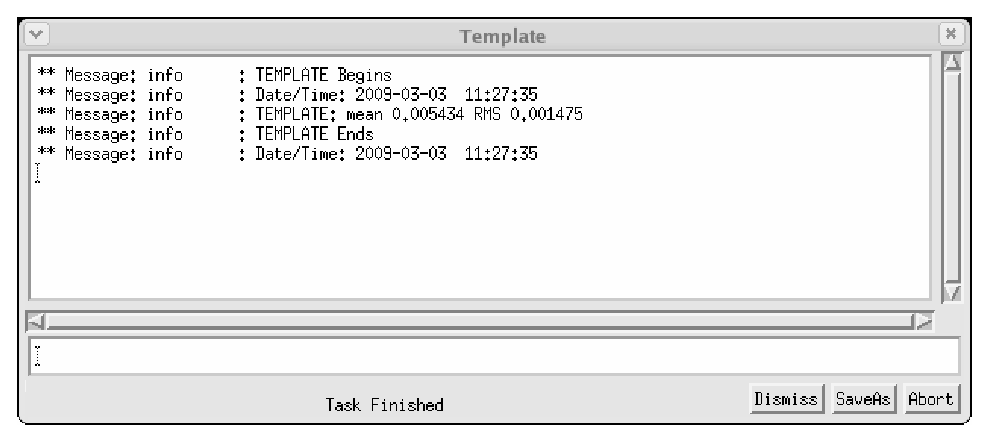
\includegraphics[height=3in]{ObitMessScreen.eps}
\caption{ 
Message window for Obit task Template after completion.
}
\label{MessWinFig}
\end{figure}

The TaskWindow object returned when an asynchrous task is started can
be used to suspend python operations until the task completes:
\begin{verbatim}
>> window.wait()
\end{verbatim}
or abort the task:
\begin{verbatim}
>> window.abort()
\end{verbatim}

Tasks (or scripts) can also be run asynchronously without a runtime
display of the messages.
This is done using the  MsgBuf argument to the go function which will then
execute the task (or script) and save the messages.
In this case the go function returns a TaskMsgBuffer.
The task messages can be saved to a logfile or obtained from the 
TaskMsgBuffer object:
\begin{verbatim}
>> buffer = go(myTask,MsgBuf=True)
>> buffer.wait()
>> messages = buffer.Messages()
\end{verbatim}
TaskMsgBuffer objects also have an abort function.

\subsection{Disk Numbers and Task Executation \label{Disks}}
``Data disks'' as defined in ObitTalk include the information about
the location of the data and ObitTalk will attempt to execute the task
where the data defined for it resides.
This means that disk numbers cannot be defaulted as then ObitTalk
cannot decide where to execute the task or tell if all data reside on
the same host.
For Obit Tasks operating on FITS files, disk 0 has a special meaning,
that the filename given is relative to the current working directory.

\subsection{Scripts}
Scripts can be executed locally directly as a command line argument to
ObitTalk or interactively using the ObitScript class (see Section
\ref{ObitScript}). 
When a script is executed from the command line, there is no prompt for
the AIPS user number which must be supplied by the script.
To use all features of the Obit python interface, a full
initialization of Obit is also needed.
An example python fragment in a script given on the command line
initializing Obit for user 100 is the following:
\begin{verbatim}
# Initialize Obit for AIPS user 100
user=100
from OTObit import *
AIPS.AIPS.userno=user
OSystem.PSetAIPSuser (user) 
err=OErr.OErr()
\end{verbatim}

Scripts can run from an interactive ObitTalk session (started with no
arguments) and can be run synchronously or asynchronously and either
locally or remotely using the ObitScript class.
Remote ObitScripts have full access to the functionality afforted
locally visible data, which it is to the script.


\subsection{Task logs}
Messages from running AIPS or Obit tasks will appear in the python
window if the task is being run synchronously or in the Task Window
if run asynchronously.
Each Task window has a button that allows writing the contents into a
file; otherwise the logging messages are lost when the window closes.
If logging to a file is desired, set the name of the file (relative or
full path) on the task object's logFile member:
\begin{verbatim}
>>> im.logFile="myLog.log"
\end{verbatim}
This will cause the messages to be logged as the task runs.

For batch, script--driven processing it may be desirable to write
messages directly to the log file from the task and not to the
terminal output or Message Server. 
This also avoids the problems of ObitTalk occasionally losing or
mangling messages or causing the task to hang due to a full I/O
buffer. 
Obit tasks can invoke direct logging using the taskLog task object
member: 
\begin{verbatim}
>>> im.taskLog="myLog.log"
\end{verbatim}

\subsection{ObitTalk/Obit routines}
ObitTalk has python binding to the Obit c library that allow access to
data and many high level functions.
Thus, scripts or interactive use can be controlled by data values in
files.
(Note: in general functions which manipulate data require that the
data be visible locally whereas tasks and the ObitTalk Data classes do
not). 

Control parameters to Obit (c) routines are largely passed in an
InfoList structure (a type of associative array similar to a python
dict) but many of the python interface routines take care of this
detail and their parameters are passed through a python dictionary.
Details are available via the python help command.
Use of ObitTalk routines is described below.

\subsection{Messages and error handling}
In ObitTalk error handling and messages use the OErr class.
ObitTalk defines a variable err at startup for this purpose.
Python functions bound to Obit routines which can generate either
messages or error conditions are passed an OErr argument.
Messages are generally not shown until explicitly requested, this
allows suppressing messages when necessary.

{\bf Note: if an error condition is indicated on err and has not been
cleared and/or messages displayed, then subsequent functions passed
err will simply return withoutperforming their function.}

OErr functions include:
\begin{itemize}
\item {\bf ShowErr(err)} Display any messages and clear any error conditions.
\item {\bf OErr.PClear(err)} Clear Obit error stack err and error condition
\item {\bf OErr.PIsErr(err)} Tells if an error condition exists
\item {\bf OErr.PLog(err, eCode, message)} Add message To Obit
Error/message stack err
\item {\bf OErr.PSet(err)} Set Obit error flag
\item {\bf OErr.printErr(err)} Prints Obit error/message stack
\item {\bf OErr.printErrMsg(err, message='Error')} Prints Obit error
stack and throws runtime exception on error 
\item {\bf OErr.OErrIsA(err)} Tells if object thinks it's a Python ObitErr
\end{itemize}

Each OErr message has a severity level:
\begin{itemize}
\item {\bf OErr.Info} Informative message
\item {\bf OErr.Warn} Warning message (not an error)
\item {\bf OErr.Traceback} Traceback information from c routines.
\item {\bf OErr.MildError} Error (but may not be serious)
\item {\bf OErr.Error} Error message
\item {\bf OErr.StrongError} Serious error
\item {\bf OErr.Fatal} Program cannot continue
\end{itemize}

\subsection{Lock and Parameter Files}
ObitTalk uses files in /tmp to indicate that resources are allocated
and for input and output parameter files for ObitTasks.
If problems occur then these files may not be properly disposed of and
may need to be deleted by hand.
These will have names like Obit\_pops\_no\_.pid (e.g. Obit3.5942)
indicating an allocated ``POPS number'' or ObitTask\_Input.pops\_no
(e.g. SCMapInput.1) indicating the input parameter file to an Obit
Task (SCMap).

\subsection{Modifying Data Headers}
The Obit/python interface can be used to modify data headers through
the Descriptor classes (ImageDesc, UVDesc, etc).  
The actual memory resident structure is a c structure which can be
translated to and from a python dict.
The general procedure is 
\begin{enumerate}
\item Open the object Read/Write
\begin{verbatim}
>>>  help(x.Open)
Open(self, access, err, blc=None, trc=None) method of Image.Image instance
    Open an image persistent (disk) form
    
    self   = Python Image object
    access    = access READONLY (1), WRITEONLY (2), READWRITE(3)
    err       = Python Obit Error/message stack
    blc       = if given and a list of integers (min 2) giving
    bottom left corner (1-rel) of subimage
    trc       = if given and a list of integers (min 2) giving
    top right corner (1-rel) of subimage
\end{verbatim}
\item Obtain the descriptor in python dict form using the x.Desc.Dict
function.
\item Modify the contents of the dict making sure to maintain its
structure, format of date strings and data types.
\item Update the Descriptor using a x.Desc.Dict = dict type statement
\item Update descriptor in external representation using the data
  object's UpdateDesc function.
\begin{verbatim}
UpdateDesc(self, err, Desc=None) method of Image.Image instance
    Update any disk resident structures about descriptor
    
    self      = Python Image object
    err       = Python Obit Error/message stack
    Desc      = Descriptor, if None then use current descriptor
                Contents can be accessed through the Dict member
\end{verbatim}
\item Close object
\end{enumerate}

An example is shown in the following in which the value of
``observer'' is changed from ``Axxxx'' to ``my code'':
\begin{verbatim}
>>> x=getname(17)
AIPS Image W3           VLA    1 1
>>> imhead(x)
AIPS Image Name: W3           Class: VLA    seq:        1 disk:    1
Object: W3      
Observed: 1992-07-17 Telescope:  VLA      Created: 2006-09-25
Observer: Axxxx      Instrument: VLA      
Minimum =       -0.018  Maximum =         2.452 JY/BEAM 
--------------------------------------------------------------
Type    Pixels   Coord value     at Pixel     Coord incr   Rotat
RA---SIN   320   2 25 36.44334     161.00       -1.72914    0.00
DEC--SIN   320  62  6 11.2407      161.00        1.72914   -0.35
FREQ         1      8.6697e+09       1.00    6.05469e+06    0.00
STOKES       1      IPol             1.00              1    0.00
--------------------------------------------------------------
Coordinate equinox 2000.0  Coordinate epoch 2000.00
Observed RA    2 25 36.44334 Observed Dec  62  6 11.2407 
no. Comp        1
Clean Beam    6.99984 x    6.99984 asec, PA     0.0 deg.
Rest freq            0 Vel type: Observer,  wrt  Optical
Alt ref value   1.1704e+05  wrt pixel    16.00
Maximum version number of AIPS CC tables is 1 
Maximum version number of AIPS HI tables is 1 

>>> x.Open(Image.READWRITE,err)
>>> d=x.Desc.Dict
>>> d["observer"]
'Axxxx   '
>>> d["observer"]="my code"
>>> x.Desc.Dict=d
>>> x.UpdateDesc(err)
>>> x.Close(err)
>>> imhead(x)
AIPS Image Name: W3           Class: VLA    seq:        1 disk:    1
Object: W3      
Observed: 1992-07-17 Telescope:  VLA      Created: 2006-09-25
Observer: my code    Instrument: VLA      
Minimum =       -0.018  Maximum =         2.452 JY/BEAM 
--------------------------------------------------------------
Type    Pixels   Coord value     at Pixel     Coord incr   Rotat
RA---SIN   320   2 25 36.44334     161.00       -1.72914    0.00
DEC--SIN   320  62  6 11.2407      161.00        1.72914   -0.35
FREQ         1      8.6697e+09       1.00    6.05469e+06    0.00
STOKES       1      IPol             1.00              1    0.00
--------------------------------------------------------------
Coordinate equinox 2000.0  Coordinate epoch 2000.00
Observed RA    2 25 36.44334 Observed Dec  62  6 11.2407 
no. Comp        1
Clean Beam    6.99984 x    6.99984 asec, PA     0.0 deg.
Rest freq            0 Vel type: Observer,  wrt  Optical
Alt ref value   1.1704e+05  wrt pixel    16.00
Maximum version number of AIPS CC tables is 1 
Maximum version number of AIPS HI tables is 1 
\end{verbatim}

\subsection{Object parameter lists\label{ParmList}}
It is frequently necessary to pass parameters to Obit functions to
control their behavior.
These are sometimes explicit arguments of python functions but in
other cases they are passed through the InfoList member of the object.
This is particularly used for data selection and calibration
parameters.
An InfoList is conceptually similar to a python dict structure
although less flexible.
An InfoList is a list of labeled data items, each item is a scalar or
an array of a given data type.
The data types supported are int, long (explicitly 32 bit in c),
float, double (explicitly 64 bit in c), boolean and strings.
More details can be obtained by viewing the help function on the
class.

Obit data (and other) objects will have an InfoList member which can
generally be accessed through the List member.
Conversion to and from python dict structures is by means of the Dict
member of the InfoList class.
Simple access to entries in an InfoList are through the set and get
functions.
\begin{verbatim}
set(self, name, value, ttype=None) method of InfoList.InfoList instance
    Save a value in an InfoList
    
    Set an entry in an InfoList, possibly redefining its type and dimension
    self     = input Python InfoList
    name     = name of desired entry
    value    = value to save, either a scalar integer, float, boolean or string
               or a 1D array of one of these types
               Type and dimensionality determined from value unless ttype is set
    ttype     = data type, "double", "long", None=>type of value
\end{verbatim}

\begin{verbatim}
get(self, name) method of InfoList.InfoList instance
    Retrieve a value from an InfoList
    
    returns python list containing data:
    0 - return code, 0=OK else failed
    1 - name
    2 - type
        int=1, oint=3, long=4, float=9, double=10, string=13, boolean=14
    3 - dimension array as list, e.g. [1,1,1,1,1] for scalar
    4 - data array
    self     = input Python InfoList
    name     = name of desired entry
\end{verbatim}

Usage of these functions as shown in the following in which x is an Obit data
object.
\begin{verbatim}
>>> x.List.set("fvalue",1.234)
>>> x.List.get("fvalue")
[0, 'fvalue', 9, [1, 1, 1, 1, 1], [1.2339999675750732]]
>>> x.List.set("farray",[1.234,4.567,7.890])
>>> x.List.get("farray")
[0, 'farray', 9, [3, 1, 1, 1, 1], [1.2339999675750732, 4.5669999122619629, 7.8899998664855957]]
>>> x.List.set("darray",[1.234,4.567,7.890],"double")
>>> x.List.get("darray")
[0, 'darray', 10, [3, 1, 1, 1, 1], [1.234, 4.5670000000000002,
    7.8899999999999997]]

>>> x.List.Dict
{'DISK': [2, [1, 1, 1, 1, 1], [1]], 'FileType': [2, [1, 1, 1, 1, 1],
    [1]], 
'fvalue': [9, [1, 1, 1, 1, 1], [1.2339999675750732]], 
'darray': [10, [3, 1, 1, 1, 1], [1.234, 4.5670000000000002,
    7.8899999999999997]], 
'User': [2, [1, 1, 1, 1, 1], [100]], 
'farray': [9, [3, 1, 1, 1, 1], [1.2339999675750732,
    4.5669999122619629, 7.8899998664855957]], 
'CNO': [2, [1, 1, 1, 1, 1], [40]], 
'Disk': [2, [1, 1, 1, 1, 1], [1]], 'nVisPIO': [2, [1, 1, 1, 1, 1], [1]]}
>>> 
\end{verbatim}

\subsection{Accessing UV Data \label {UVData}}
There are a number of Obit Class functions that perform highlevel
operations of uv data sets (UV objects) in the CleanVis, 
UVImager, and UVSelfCal classes.
For details, import these classes and view the help documentation.
Visibility data can be read from and written to data objects using the
UV ReadVis and WriteVis functions employing objects of the UVVis
class.

The selection, calibration and editing of visibility data can be
controlled by setting parameters on the InfoList member of the UV data
object. 
Many of these are set using the interface to highlevel class
functionality, but for a given parameter which is not part of the
class function interface definition, the value can be set directly
through the InfoList (see section \ref{ParmList}).
A complete list of the UV data selection/calibration/editing
parameters follows. 

\begin{itemize}
\item  doCalSelect boolean scalar\\
Select/calibrate/edit data?
\item  Stokes string (4,1,1) \\
Selected output Stokes parameters:
``    "$\Rightarrow$ no translation,"I   ","V   ","Q   ", "U   ", 
"IQU ", "IQUV",  "IV  ", "RR  ", "LL  ", "RL  ", "LR  ", 
"HALF" = RR,LL, "FULL"=RR,LL,RL,LR. [default "    "]
For data with linear feeds substiture ``X'' and ``Y'' for ``R'' and ``L''.
In the above 'F' can substitute for "formal" 'I' (both RR+LL or XX+YY).
\item  BChan int scalar \\ 
First spectral channel (1-rel) selected. [def all]
\item  EChan int scalar \\ 
Highest spectral channel (1-rel) selected. [def all]
\item  BIF   int scalar \\ 
First IF (1-rel) selected. [def all]
\item  EIF   int scalar \\ 
Highest IF (1-rel) selected. [def all]
\item  doPol   int scalar \\ 
$>0 \Rightarrow$ calibrate polarization.
\item  PDVer   int scalar \\ 
PD table version.
\item  doCalib int scalar \\ 
$>0 \Rightarrow$ calibrate, $2 \Rightarrow$ also calibrate Weights
\item  gainUse int scalar \\ 
SN/CL table version number, $0 \Rightarrow$ use highest
\item  flagVer int scalar \\ 
Flag table version, $0 \Rightarrow$ use highest, $<0 \Rightarrow$ none
\item  BLVer   int scalar \\ 
BL table version, $0>$ use highest, $<0 \Rightarrow$ none
\item  Subarray int scalar \\ 
Selected subarray, $<=0 \Rightarrow$all [default all]
\item  dropSubA bool scalar \\ 
Drop subarray info?
\item  FreqID   int scalar \\ 
Selected Frequency ID, $<=0 \Rightarrow$all [default all]
\item  timeRange float (2,1,1) \\
Selected timerange in days.
\item  UVRange float (2,1,1) \\
Selected UV range in kilowavelengths.
\item  InputAvgTime float scalar \\ 
Input data averaging time (sec). Used for fringe rate decorrelation correction.
\item  Sources string (?,?,1) \\
Source names selected unless any starts with
a '-' in which case all are deselected (with '-' stripped).
\item  souCode string (4,1,1) \\
Source Cal code desired, 
\begin{itemize}
\item '    ' $\Rightarrow$ any code selected
\item '*   ' $\Rightarrow$ any non blank code (calibrators only)
\item '-CAL' $\Rightarrow$ blank codes only  (no calibrators)
\end{itemize}
\item  Qual    int scalar \\  
Source qualifier, -1 [default] = any
\item  Antennas int (?,1,1) \\
a list of selected antenna numbers, if any is negative
then the absolute values are used and the specified antennas are deselected.
\item  corrType int scalar \\
Correlation type, 0=cross corr only, 1=both, 2=auto only.
\item  passAll bool scalar \\
If True, pass along all data when selecting/calibration
even if it's all flagged.  
Data deselected by time, source, antenna etc. is not passed.
\item  doBand  int scalar \\
Band pass application type $<0 \Rightarrow$ none:
\begin{enumerate}
\item If = 1 then all the bandpass data for each antenna
will be averaged to form a composite bandpass
spectrum, this will then be used to correct the data.
\item If = 2 the bandpass spectra nearest in time (in a weighted
sense) to the uv data point will be used to correct the data. 
\item If = 3 the bandpass data will be interpolated in time using the
solution weights to form a composite bandpass spectrum, this
interpolated spectrum will then be used to correct the data.
\item If = 4 the bandpass spectra nearest in time (neglecting weights)
to the uv data point will be used to correct the data.
\item If = 5 the bandpass data will be interpolated in time ignoring
weights to form a composite bandpass spectrum, this interpolated
spectrum will then be used to correct the data. 
\end{enumerate}
\item  Smooth  float (3,1,1) \\
specifies the type of spectral smoothing
\begin{itemize}
 \item  Smooth[0] = type of smoothing to apply:
\begin{itemize}
\item 0 $\Rightarrow$ no smoothing
\item 1 $\Rightarrow$ Hanning
\item 2 $\Rightarrow$ Gaussian
\item 3 $\Rightarrow$ Boxcar
\item 4 $\Rightarrow$ Sinc (i.e. sin(x)/x)
\end{itemize}
\item Smooth[1] = the "diameter" of the function, i.e. width between
first nulls of Hanning triangle  and sinc function, FWHM of Gaussian,
width of Boxcar. Defaults (if $<$ 0.1) are 4, 2, 2 and 3 channels for
Smooth[0] = 1 - 4. 
\item Smooth[2] = the diameter over which the convolving function has
value - in channels. Defaults: 1, 3, 1, 4 times Smooth[1] used when
\end{itemize}
\item  BPVer   int scalar \\ 
Band pass (BP) table version, $0 \Rightarrow $use highest
\item SubScanTime float scalar \\
\{Optional\} if given, this is the desired time (days) of a sub scan.  
This is used by the selector to suggest a value close to this which will
evenly divide the current scan.  0 $\Rightarrow$ Use scan average.
This is only useful for ReadSelect operations on indexed ObitUVs.
\end{itemize}

As an example of the data selection usage, to specify that only
autocorrelations are desired in UV data object myUV in subsequent
operations: 
\begin{verbatim}
>>> myUV.List.set('corrType',2)
\end{verbatim}

\section{Parallel Processing}
   ObitTalk and Obit tasks implement some basic aspects of parallel
processing.  
These include using multiple cores and/or processors with shared
memory in a computer using multi--threading and distributing tasks
across nodes of a cluster or workstations on a LAN.
These are described in the following sections.

\subsection{Multi--threading}
Many of the more expensive operation in Obit allow using multiple
processors/cores which share memory.
The technique of multi--threading is used for this.
Obit tasks which support multi--threading have a parameter, nThreads,
giving the maximum number of threads to allow in a parallel operation.
In general, this should not be more than the actual number of
processors/cores available but may be fewer if multiple tasks are to
be run using threading or the particular task executation cannot make
good use of more than a given number of threads.
Threading in functions called from scripts can be invoked as in the
following example of allowing two parallel threads.
\begin{verbatim}
>>> # Allow multiple threads
>>> OSystem.PAllowThreads(16)  # 16 threads max.
\end{verbatim}

\subsection{GPU}
The most compute intensive operations have a GPU implementation in
cuda.
In tasks, these are invoked using the doGPU and doGPUGrid parameters.
Multiple GPU can be used for visibility data gridding using parameter
array GPU\_no.
Usage of GPUs must be implemented in a built--from--source version due
to licencing and other restrictions

\subsection{Cluster Nodes}
ObitTalk can start parallel, independent processes on multiple nodes
of a cluster of workstations on a network; these can be either tasks or
ObitScripts. 
Executation is initiated on the node/workstation on which the data
disks are defined.
See sections \ref{Disks} and \ref{Remote} for more details.

\section{Examples}
The following give simple examples of using ObitTalk.

\subsection{Display AIPS Catalog}
The examine your AIPS image catalog on disk 7
\begin{verbatim}
>>> AMcat(7)
AIPS Directory listing for disk 7
  1 CYG A 74 MHz.MODEL .    1 MA 13-Apr-2004 10:25:32     
\end{verbatim}

\subsection{Create Python Image Object}
To create a python object for the AIPS image in slot 1 and name it ``x'':
\begin{verbatim}
>>> x=getname(1,7)
AIPS Image CYG A 74 MHz MODEL  7 1
\end{verbatim}

\subsection{Display Data Header}
To view the image header of x:
\begin{verbatim}
>>> imhead(x)
AIPS Image Name: CYG A 74 MHz Class: MODEL  seq:        1 disk:    7
Object: 3C405   
Observed: 2001-01-19 Telescope:  VLA      Created: 2001-03-03
Observer: AD441      Instrument: VLA      
Minimum =          -25  Maximum =        4638.2 JY/BEAM 
--------------------------------------------------------------
Type    Pixels   Coord value     at Pixel     Coord incr   Rotat
RA---SIN   512  19 59 28.35406     256.00             -5    0.00
DEC--SIN   512  40 44  2.0862      257.00              5    0.32
FREQ         1        7.38e+07       1.00    1.55029e+06    0.00
STOKES       1      IPol             1.00              1    0.00
--------------------------------------------------------------
Coordinate equinox 2000.0  Coordinate epoch 2000.00
Observed RA   19 59 28.35406 Observed Dec  40 44  2.0862 
no. Comp      697
Clean Beam    24.9998 x    24.9998 asec, PA     0.0 deg.
Rest freq            0 Vel type: Observer,  wrt  Optical
Alt ref value            0  wrt pixel     0.00
Maximum version number of AIPS CC tables is 1 
Maximum version number of AIPS HI tables is 1 
\end{verbatim}

\subsection{Display an Image}
To display image x in ObitView:
\begin{verbatim}
>>> tvlod(x)
\end{verbatim}
Note: if ObitTalk thinks something has gone wrong with the image
display, the python object may need to be recreated.
To recreate the default image display:
\begin{verbatim}
>>> newDisplay()
\end{verbatim}

\subsection{Image Pixel Access}
Access to arrays of image pixel values is through the FArray class.
Images can be read into or written from FArray objects which can be
manipulated in many ways.
See help(FArray) for details.
In the following the pixel array in an image is read and several
operations are performed.
\begin{verbatim}
>>> # Create image object from AIPS catalog entry
>>> x = Image.newPAImage("Swan","Cygnus A","J2000",1,1,True,err)
>>> ShowErr(err)                # Check for errors
>>> x.Open(Image.READONLY,err)  # Open image
>>> x.Read(err)                 # Read plane
>>> pixels=x.FArray             # python FArray object from image
>>> pixels.Mean                 # Display Mean of pixel values
49.573715209960938 
>>> pixels.RMS                  # Display RMS of pixel values
4.758549690246582
>>> FArray.PSMul(pixels, 5.0)   # Scale all pixels by 5
>>> pixels.Mean                 # Display new mean
247.86857604980469
>>> x.Close(err)                # Close image
>>> pixels.get(100,100)         # Display (0-rel) pixel [100,100]
8.0
>>> pixels.set(3.1415926,100,100) # set value of pixel [100,100]
>>> pixels.get(100,100)         # See new value
3.1415925025939941

\end{verbatim}

\subsection{Run an AIPS task}
To run AIPS task IMEAN on x and view the values returned:
\begin{verbatim}
>>> imean=AIPSTask("imean")  # Define task object
>>> setname(x,imean)         # Fill in info on x to task object
>>> imean.i                  # View inputs
Adverbs     Values                                   Comments
--------------------------------------------------------------------------------
 dohist      -1.0                                     True (1.0) do histogram plot.
                                                      = 2 => flux on x axis
 userid       0.0                                     User ID.  0=>current user
                                                        32000=>all users
 inname      CYG A 74 MHz                             Image name (name)
 inclass     MODEL                                    Image name (class)
 inseq        1.0                                     Image name (seq. #)
 indisk       7.0                                     Disk drive #
 blc         0.0, 0.0, 0.0, 0.0, 0.0, 0.0, 0.0        Bottom left corner of image
                                                        0=>entire image
 trc         0.0, 0.0, 0.0, 0.0, 0.0, 0.0, 0.0        Top right corner of image
                                                        0=>entire image
 nboxes       0.0                                     No. of ranges for histogram.
 pixrange    0.0, 0.0                                 Min and max range for hist.
 functype                                             'LG' => do log10 plot of #
                                                      samples, else linear
 pixavg       0.0                                     Estimate of mean noise value
 pixstd       0.0                                     Estimate of true noise rms
                                                         < 0 => don't do one
                                                         = 0 => 2-passes to get
 docat        1.0                                     Put true RMS in header
 ltype        3.0                                     Type of labeling: 1 border,
                                                      2 no ticks, 3 - 6 standard,
                                                      7 - 10 only tick labels
                                                      <0 -> no date/time
 outfile                                              Name of output log file,
                                                      No output to file if blank
 dotv        -1.0                                     > 0 Do plot on the TV, else
                                                      make a plot file
 grchan       0.0                                     Graphics channel 0 => 1.

>>> imean.g       # Execute task
IMEAN1: Task IMEAN  (release of 31DEC02) begins
IMEAN1: Image= CYG A 74 MHz.MODEL .   1 7   xywind=    1    1  512  512
IMEAN1: Mean and rms found by fitting peak in histogram:
IMEAN1: Mean= 4.8010E-02 Rms= 4.7438E+00  **** from histogram
IMEAN1: Mean and rms found by including all data:
IMEAN1: Mean= 1.8457E+00 Rms= 6.0963E+01 JY/BEAM  over    262144 pixels
IMEAN1: Flux density =  1.7080E+04 Jy.   beam area =  28.33 pixels
IMEAN1: Minimum=-2.5000E+01 at   59  145    1    1
IMEAN1: Skypos: RA 20 00 55.087  DEC 40 34 45.54
IMEAN1: Maximum= 4.6382E+03 at  252  256    1    1
IMEAN1: Skypos: RA 19 59 30.116  DEC 40 43 57.20
IMEAN1: Skypos: IPOL  73.800 MHZ
IMEAN1: returns adverbs to AIPS
IMEAN1: Appears to have ended successfully
IMEAN1: smeagle      31DEC06 TST: Cpu=       0.0  Real=       0

>>> imean.o     # Examine outputs
Adverbs     Values                                   Comments
--------------------------------------------------------------------------------
 pixavg      0.0480099283159                          Estimate of mean noise value
 pixstd      4.74377298355                            Estimate of true noise rms
                                                         < 0 => don't do one
                                                         = 0 => 2-passes to get
\end{verbatim}

\subsection{Run an Obit task (FndSou)}
To run Obit task FndSou on an image, x, containing multiple sources to
generate a source catalog (use sf.h for detailed help):
\begin{verbatim}
>>> sf=ObitTask("FndSou")
>>> setname(x,sf)
>>> sf.outDisk=1
>>> sf.NGauss=20      # Max. number of sources (islands)
>>> sf.CutOff=2       # Minimum pixel brightness to consider
>>> sf.Retry=1        # Try multiple components if residuals exceed this
>>> sf.doMult=True    # Allow using multiple Gaussians per source
>>> sf.doWidth=True   # Fix width
>>> sf.Parms=[2., 5., 0., 1]
>>> sf.RMSsize=50     # Size of window to use to determine image RMS
>>> sf.prtLv=1        # Some diagnostic output
>>> sf.doVL=True      # Generate VL table
>>> sf.i              # Display inputs
FndSou:  Task to fit Gaussian models to an image by least-squares
Adverbs     Values                                   Comments
--------------------------------------------------------------------------------
 DataType    AIPS                                   FITS" or "AIPS" type of input
 inName      1400+208                               Image Name (Name) 1
 inClass     ICLEAN                                 Image Name (Class) 1
 inSeq          1                                   Image Name (Seq. #) 1
 inDisk         1                                   Disk drive # 1
 inFITS                                             Filename 1 if FITS image
 BLC         0, 0, 0, 0, 0, 0, 0                    Bottom left corner of image
                                                      0=>entire image
 TRC         0, 0, 0, 0, 0, 0, 0                    Top right corner of image
                                                      0=>entire image
 doVL        True                                   Convert to VL table?
 doPBCorr    False                                  PB correction to VL table?
 asize       25.0                                   antenna diam. for PB corr.
 doResid     False                                  Catalog residual map?
 outName                                            Output Image Name
 outClass                                           Output Image Class
 outSeq         0                                   Output Image Seq. #
 outDisk        1                                   output Disk drive
 outFITS                                            Output Filename if FITS image
 NGauss        20                                   Max. Number of islands
 NPass          1                                   Number of passes through resid.
 CutOff       2.0                                   Flux cutoff level
 Retry        1.0                                   Retry level
 Sort                                               Sort Order of output ' '=RA
 OutPrint                                           Printer disk file to save
 doMult      True                                   >0 => fit multiple peaks
 doWidth     True                                   >0 => fit widths
 Gain        0.05                                   Amp-dependent part of retry
                                                    and warning levels
 Parms       2.0, 5.0, 0.0, 1.0, 0.0                Components constraints
                                                    [0] flux < Parms[0]
                                                    [1] widths>Parms[1] cells
                                                    [2] peaks>Parms[2] cells
                                                    outside fitting region
                                                    [3] if >0 don't allow Gauss
                                                    smaller than CLEAN beam
 RMSsize       50                                   Size of region to determine RMS
 prtLv          1                                   Debug print level

>>> sf.g              # run task 
** Message: info      : FndSou Begins
** Message: info      : Date/Time: 2007-10-11  13:47:51
** Message: info      : Found 23 islands pass 1
** Message: info      : Successfully fitted 20 components
** Message: info      : Attempt to break 0 islands into multiple
** Message: info      : 0 Attempts to break islands failed
** Message: info      : 0 components rejected for low peak
** Message: info      : 0 fits hit iteration limit
Found 23 islands in 1 passes
Successfully fitted 20 components
Attempt to break 0 islands into multiple
0 Attempts to break islands failed
0 components rejected for low peak
0 fits hit iteration limit

   ...

** Message: info      : FndSou Ends
** Message: info      : Date/Time: 2007-10-11  13:47:58
\end{verbatim}

\subsection{Table Access (print contents of VL table)}
To create a python object from the VL table created in the previous example
and display its contents using the Catalog module utility PVLPrint:
\begin{verbatim}
>>> import Catalog
>>> vltab=x.NewTable(Table.READONLY, "AIPS VL",1,err)
>>> Catalog.PVLPrint(vltab,x,err)
>>> ShowErr(err) # Display any error messages

 Listing of fitted VL table values
Fitted sizes in asec, Peak, Flux, IRMS in mJy, residual values relative to Peak
Error estimates (asec, mJy, deg) given under value
             RA           Dec          Peak    Flux    IRMS  Fit Maj Fit min 
    1  13 43 56.1032   22 18 21.163  3666.31  4806.81  90.186 104.886  80.000
                1.80           1.12    93.92   123.13           3.021   1.822
    2  13 48 14.5900   24 15 57.461  5508.17  5917.91  87.870  85.951  80.000
                0.82           0.81    89.29    95.93           1.442   1.253
    3  13 48 51.8784   26 35 44.011  2742.81  3484.55  77.721  98.355  82.667
                1.60           1.69    81.18   103.13           3.143   2.266
    4  13 49 39.0137   21 07 29.926 13631.90 13820.04 112.454  81.104  80.000
                0.41           0.40   112.83   114.39           0.676   0.658
    5  13 50 58.3986   15 51 55.507  2479.43  2733.85  91.272  88.209  80.000
                1.94           1.88    93.20   102.76           3.473
   ...
\end{verbatim}

\subsection{Table Row Data}
In the following example, the header of an AIPS CC (Clean Components) 
table is converted to a dict and printed and the first few rows 
are read into a python dict structure and printed.
\begin{verbatim}
>>> imDict=x.Desc.Dict
>>> xinc = abs(imDict['cdelt'][0])   # X Cell spacing
>>> yinc = abs(imDict['cdelt'][1])   # Y Cell spacing
>>> cctab=x.NewTable(Table.READONLY,"AIPS CC",1,err)
>>> thead=cctab.Desc.Dict
>>> thead   # Display contents of python dict
{'repeat': [1, 1, 1, 1], 'nrow': 114, 'dim1': [1, 1, 1, 1],
'sortOrder2': 0, 'sortOrder1': 0, 'dim2': [1, 1, 1, 1], 
'dim0': [1, 1, 1, 1], 'version': 1, 'lrow': 16, 'Table name': 'AIPS CC', 
'FieldName': ['FLUX', 'DELTAX', 'DELTAY', '_status'], 
'type': [9, 9, 9, 2], 'FieldUnit': ['JY', 'DEGREES', 'DEGREES', '']}

>>> cctab.Open(Table.READONLY,err)
>>> ShowErr(err) # Display any error messages
>>> for i in range(1,5):    # Loop over first 4 rows printing
...     row = cctab.ReadRow(i, err)    # Read row i (1-rel)
...     xcell = row["DELTAX"][0]/xinc  # X position in cells
...     ycell = row["DELTAY"][0]/yinc  # Y position in cells
...     flux  = row["FLUX"][0]         # Flux
...     print "%5d %5.2f %5.2f %10.2f" % (i,xcell, ycell,flux)
... 
    1 -16.00  6.00    1260.95
    2 -47.00 16.00     646.20
    3 -16.00  5.00     626.66
    4 -46.00 16.00     527.65
>>> cctab.Close(err)                   # Close table

\end{verbatim}

\subsection{Writing to a History}
The following example writes a timestamp and a comment into a image
processing history and then prints the history.
\begin{verbatim}
>>> hi = x.History(Image.READWRITE, err)       # Extract history object from image
>>> r=hi.Open(History.READWRITE, err)          # Open history
>>> hi.TimeStamp(" Start Obit "+ObitSys.pgmName,err) # Timestamp
>>> r=hi.WriteRec(-1,"Some comment",err)       # write comment
>>> r=hi.Close(err)                            # Close
>>> OErr.printErrMsg(err, "Error with history")# Error test
>>> PrintHistory(x)                            # Show history
History for AIPS:Image:Cygnus A.J2000.1.1
     1 --------------------------------------------------------------------  
     2 --------------------------------------------------------------------  
     3 /Begin "HISTORY" information found in fits tape header by IMLOD       
...
  1553         / 2007-10-11T21:12:11  Start Obit ObitPython
  1554 Some comment
\end{verbatim}

\subsection{Modify Visibility Data}
The UV functions ReadVis and WriteVis read and write single visibility
records in the form of python UVVis objects which contain the
following members:
\begin{itemize}
\item {\bf u}    u coordinate (lambda)
\item {\bf v}    v coordinate (lambda)
\item {\bf w}    w coordinate (lambda)
\item {\bf time} Visibility time in days since 0 h on reference day
\item {\bf ant1} antenna 1 of baseline
\item {\bf ant2} antenna 2 of baseline
\item {\bf vis } visibilities as list of tuples (vis, wt) as (complex, float)
\end{itemize}

The visibilities are in the order defined in the data descriptor:
\begin{itemize}
\item {\bf jlocs} 0-rel axis order: Stokes' parameters
\item {\bf incs} Increment in data: Stokes (in floats)
\item {\bf jlocf} 0-rel axis order: Frequency
\item {\bf incf} Increment in data: Frequency (in floats)
\item {\bf jlocif} 0-rel axis order: IF
\item {\bf incif} Increment in data: IF (in floats)
\end{itemize}

   The following example uses the UVVis class to read the records in a
UV data file, multiply the complex visibilities by 2.0 and the weights
by 0.5.
To specify data selection, calibration and editing to be applied to
data as it is read, see section \ref{UVData}.
\begin{verbatim}
# Input AIPS file
x = UV.newPAUV("inUV", "RX_Tau", "IF2", 1, 1, True,err, nvis=1)
x.Open(UV.READONLY, err)
OErr.printErrMsg(err, "Error with input image")
# Output AIPS file
y = UV.newPAUV("outUV", "RX_Tau", "Copy", 1, 1, False,err, nvis=1)
UV.PClone(x, y, err)
y.Open(UV.WRITEONLY, err)
OErr.printErrMsg(err, "Error with output image")

# Get information about data
nvis  = x.Desc.Dict["nvis"]           # Number of visibilities
jstok = x.Desc.Dict["jlocs"]          # Order in data of Stokes
nstok = x.Desc.Dict["inaxes"][jstok]  # Number of Stokes (polarizations)
stokinc = x.Desc.Dict["incs"]/3       # Increment between Stokes in vis
jfreq = x.Desc.Dict["jlocf"]          # Order in data of Frequency
nfreq = x.Desc.Dict["inaxes"][jfreq]  # Number of Frequencies
freqinc = x.Desc.Dict["incf"]/3       # Increment between channels in vis
jif   = x.Desc.Dict["jlocif"]         # Order in data of IF
nif   = x.Desc.Dict["inaxes"][jif]    # Number of IFs
ifinc = x.Desc.Dict["incif"]/3        # Increment between IFs in vis

# Loop over input file
for i in range(0, nvis):    
    # read to UVVis
    v = x.ReadVis(err)
    vlist = v.vis  # array of tuples (complex vis, float weight)
    # Multiply each vis by two, multiply weight by 0.5
    # Loop over IF
    for iif in range (0, nif):
        # Loop over Frequency channel
        for ifreq in range (0, nfreq):
            # Loop over Stokes
            for istok in range (0, nstok):
                indx = istok*stokinc + ifreq*freqinc + iif*ifinc
                # Extract visibility tuple
                tup = vlist[indx]
                vlist[indx] = (2.0*tup[0],tup[1]*0.5)  # multiply/replace
    # Write data to output
    y.WriteVis(v, err)
    OErr.printErrMsg(err, "Error copying file")

# Close files
x.Close(err)
y.Close(err)
OErr.printErrMsg(err, "Error closing file")
\end{verbatim}

\subsection{Write Quantized FITS image}
   The following example reads an AIPS image and writes a integerized FITS
image with the pixel values truncated at a set fraction of the RMS "noise"
in the image.  This operation creates an image which is more compressible
but with a controlled loss of precision.
Note: in practice is is better to use the ObitTalk function imtab as
it is simpler to use and will also copy tables; this example is given
to show how to access images in ObitTalk.

\begin{verbatim}
# Specify input and output
inDisk   = 1
Aname    = "INPUT IMAGE"
Aclass   = "CLASS"
Aseq     = 1
outDisk  = 1
outFile  = "Quantized.fits"

# Create Images
inImage   = Image.newPAImage("Input image", Aname, Aclass, inDisk, Aseq, True, err)
# Note: inImage can also be created using getname(cno,disk)
outImage  = Image.newPFImage("Output image",   outFile,  outDisk,  False, err)
Image.PClone(inImage, outImage, err)   # Same structure etc.
OErr.printErrMsg(err, "Error initializing")

# Fraction of RMS 
fract = 0.25

# Copy to quantized integer image with history
inHistory  = History.History("history", inImage.List, err)
Image.PCopyQuantizeFITS (inImage, outImage, err, fract=fract, inHistory=inHistory)
OErr.printErrMsg(err, "Writing to FITS")
\end{verbatim}

%\end{alltt}\
\subsection{Subtract a CLEAN model from UV Data}
The following python script fragment subtracts the Fourier transform
of a CLEAN model, multiplied by 0.5 from one uv data set and writes
another.
Several steps are necessary to create a SkyModel from an image mosaic
containing a single image.
Then, control parameters are entered into the input dict for
SkyModel.PSubUV which is used to perform the operation.
The input and output data are all FITS files with names inFile,
inModel, outFile on FITS ``disks'' inDisk and outDisk.
Note: this operation is more simply performed by task UVSub.
\begin{verbatim}
import SkyModel, ImageMosaic
# Set data
inData  = UV.newPFUV("Input uv data", inFile, inDisk, True, err)
inImage = Image.newPFImage("Input image",inModel, inDisk, True, err)
outData = UV.newPFUV("Output uv data", outFile, outDisk, False, err)
OErr.printErrMsg(err, "Error initializing")

# Make Image Mosaic with a single image
mosaic = ImageMosaic.newObit("Mosaic", 1, err)
OErr.printErrMsg(err, "Error making mosaic")

# Add image to mosaic
ImageMosaic.PSetImage(mosaic, 0, inImage)

# Make SkyModel from mosaic
model = SkyModel.PCreate("SkyModel", mosaic)
OErr.printErrMsg(err, "Error making SkyModel")

# Control parameters to input dict, most defaulted
Input = SkyModel.UVSubInput
Input['InData']      = inData   # Input uv data
Input['SkyModel']    = model    # SkyModel
Input['OutData']     = outData  # output uv data
Input['doCalSelect'] = False    # No calibration or data selection
Input['Stokes']      = '    '   # No conversion of Stokes
Input['Factor']      = 0.5      # Multiply model FT by 0.5
Input['Mode']        = 0        # Fastest FT type (DFT or Grid)
Input['Type']        = 0        # Use CLEAN model from CC table
Input['CCVer']       = [2]      # Use CC table 2 (array of 1 per image)

# Subtract Fourier transform of sky model from inData, write outData
SkyModel.PSubUV(err, Input)
OErr.printErrMsg(err, "Error subtracting")
\end{verbatim}

\subsection{Image Gaussian Fitting}
Fitting of Gaussians to an image over a large area can be performed by
task FndSou and over more limited areas using the ImageFit class
function Fit.  
This function takes an image and a FitRegion which defines the fitting
area of the image and the initial set of values defining the Gaussians
to be fit.
Image class functions TVFit and GaussFit provide a simplified
interface to the fitting routines.

The following is an example of an interactive model fitting session, a
screen shot of the ObitView window after the fitting region and model
are specified is shown in figure \ref{ImageFitFig}

\begin{figure}
\centering
\includegraphics[angle=-90,origin=c,height=3in]{ImageFit.eps}
\caption{ 
Screenshot of ObitView window specifying fitting region with model.
}
\label{ImageFitFig}
\end{figure}
\begin{verbatim}
>>> # Define image
>>> x=Image.newPAImage("image","3C84","PennAr",1,1,True,err)
>>> # Interactively set fitting region followed by fitting
>>> fr = x.TVFit(x,disp,err)
\end{verbatim}
The image will be loaded to the display, hit the ``edit'' button on
the RequestBox, then specify the region to fit on the display with a
rectangular box, followed by circular boxes to mark Gaussian components
initial locations and initial sizes; instructions are given in the
ObitView Message Box.
When done, hit ``d'' and then ``OK'' on the bottom of the RequestBox.
Example results:
\begin{verbatim}
Model fit for 3C84    
RA     3 19 47.73316 (   0.518 asec),  pixel  131.441 (   0.259)
Dec   41 30 36.7370  (   0.594 asec),  pixel  116.772 (   0.297)
Peak Flux density   0.0109 (0.000725) JY/BEAM 
Integrated Flux density   0.0164 ( 0.00109) Jy
Fitted Major axis   15.148 (    1.13) asec,    7.574 (    0.33) pixels
Fitted Minor axis   11.228 (   0.661) asec,    5.614 (    0.33) pixels
Fitted Position angle  -36.995 (    7.84) deg
\end{verbatim}

\begin{verbatim}
Deconvolved model
Deconvolved Major axis     10.8 (    1.12) asec,    5.385 (   0.814) pixels
Deconvolved Minor axis     3.55 (    1.63) asec,    1.776 (   0.814) pixels
Deconvolved Position angle   143.01 (    5.49) deg
\end{verbatim}

Image class function GaussFit can be used for noninteractive fitting.
The defaults are generally adequate for a single source near the
reference pixel.  
Both TVFit and GaussFit return a FitRegion object.

Additional functionality can be obtained by using ImageFit functions directly, first 
\begin{verbatim}
>>> import ImageFit, FitRegion, FitModel
\end{verbatim}
The ImageFit.Fit function is described in the following:
\begin{verbatim}
Fit(self, err, input={'FluxLow': 0.0, 'GMajLow': 0.0, 'GMajUp': 1e+20, 
     'GMinLow': 0.0, 'GMinUp': 1e+20, 'MaxIter': 0, 'PosGuard': 0.0, 
     'fitImage': None, 'fitRegion': None, 'prtLv': 0, ...})
  Fit a model to an image
 
  Resultant model left in FitRegion reg
  inImageFit = Python ImageFit object
  image      = ObitImage to be fitted
  reg        = Fit region defining what is to be fitted and initial guess
  err        = Python Obit Error/message stack
  input      = input parameter dictionary
 
  Input dictionary entries:
  fitImage Image to be fitted
  fitRegion FitRegion to be fitted
  MaxIter  int Maximum number of iterations [def. 10 per fitted parameter]
  prtLv    int Message level, 0=>none [def 0]
  PosGuard float Distance (cells) from edge to allow center  [def no bound]
  FluxLow  float Lower bounds on Flux density [def no bound]
  GMajUp   float Major axis upper bound (cells) [def no bound]
  GMajLow  float Major axis lower bound (cells) [def no bound]
  GMinUp   float Minor axis upper bound (cells) [def no bound]
  GMinLow  float Minor axis lower bound (cells) [def no bound]
\end{verbatim}

A FitRegion can be created interactively using the image viewer and
FitRegion.PSetup():
\begin{verbatim}
PSetup(inImage, disp, err)
   Interactive initial definition of fitting region
        
  Interactively allows the user to set the region of the image
  to be fitted and the initial model.
  The fitting region is first specified with a rectangular window
  and then the initial models to be fitted with circular windows.
  Returns FitRegion, leaves image pixel array on inImage
    image  = image to be fitted
    disp   = image display to use
    err    = Obit Error/message stack

\end{verbatim}

Fitted models can then be viewed on the screen or written to a file by
FitRegion.Print()
\begin{verbatim}
  Print(self, ImDesc, file=None)
      Display human readable contents
      
      self     = object with Model to display
      ImDesc   = Image Descriptor with Beam, etc.
      file     = if present, the name of a file into which to write
                 the information rather than displaying it on the screen
\end{verbatim}
or, can be accessed in python using the array of FitModel objects in
the FitRegion.


\section{Radio Interferometry Applications}
There are a number of applications of particular interest to
interferometric imaging.
Detailed discussions of a number of related topics are given in papers
and memos referenced in \\ https://www.cv.nrao.edu/$\sim$bcotton/Obit.html.
\subsection{Calibration and Imaging Pipelines}
There are several calibration and imaging pipeline for specific
instruments available.
\subsubsection{EVLA}
A scripted calibration and imaging package for EVLA continuum observations
is  described in
https://www.cv.nrao.edu/$\sim$bcotton/ObitDoc/EVLAObitScripts.pdf.
The top level of this set of python scripts is
\$OBIT/python/EVLAContPipe.py.
This processes continuum observations, including polarization and
starts from data in ALMA SDM format.  
This can also be used for the continuum portion of spectral line datasets.

\subsubsection{ALMA}
A scripted calibration and imaging package for ALMA continuum observations
is  described in https://www.cv.nrao.edu/$\sim$bcotton/ObitDoc/ALMAScripts.pdf.
The top level of this package is in \$OBIT/python/ALMAPipe.py.

\subsubsection{VLBA}
A dated processing pipeline for VLBA continuum observations is implemented
in \\
\$OBIT/python/VLBAContPipeWrap.py.
Documentation is available in the (pretty old) files \\
https://www.cv.nrao.edu/$\sim$bcotton/ObitDoc/VLBAPipeMan.pdf and\\
https://www.cv.nrao.edu/$\sim$bcotton/ObitDoc/VLBAPipelineHeuristics.pdf.
There is also the source code for user documentation in a now defunct
language in\\
https://www.cv.nrao.edu/$\sim$bcotton/ObitDoc/VLBAPipelineUserManual.rst.

\subsection{Importing Data into AIPS Format}
There are several programs for converting external uv data formats
into AIPS format.
\begin{itemize}
\item {\bf ASDMList:} Lists the contents of an ALMA SDM format data
  set.
\item {\bf BDFIn:} This task reads EVLA or ALMA data in ALMA SDM
  format and writes AIPS or AIPS task FITAB format.
The latter is generally a bad idea as it can be VERY sloy.
\item {\bf IDIIn:} IDI format was intended to be a generic data
  interchange format for visibility data but only the VLBA and VLITE
  has adopted it.
  IDIIn converts to AIPS format.; IDIOut writes IDI format.
\end{itemize}
Task Lister with optype='SCAN' will give a listing of the contents of
a uv data set with an index (AIPS NX) table.

Note: UVFITS format must be converted by AIPS task UVLOD or FITLD.

\subsection{Data Editing}
There are a number of utilities for flagging data - marking them as
bad.
Help documentation is available for the tasks or functions.
These function by adding entries in the AIPS FG flagging
table which can be applied when accessing the associated data through
the flagVer parameter.
\begin{itemize}
\item {\bf AutoFlag:} This utility has a number of facilities for
  flagging data on criteria such as excessive amplitudes in Stokes I
  and/or polarized intensities or by excessive RMSes over a given
  time interval. 
It also includes several means of flagging data based on frequency
domain characteristics such as deviations from a running median in
frequency. 
\item {\bf MednFlag:} Flags data based on deviations from running
  medians in time.
\item {\bf UVFlag:} Flags selected data including those shadowed by
  another antenna.
\item {\bf SrvrEdt:} Flags remaining data for records in which the
  bulk of the data has been flagged and it is assumed all are bad.
\item {\bf UV.PFlag:} Function PFlag in python class UV allows
  flagging selected data directly from python.
\begin{verbatim}
PFlag(inUV, err, flagVer=1, timeRange=[0.0, 1e+20], Ants=[0, 0],
    Source='Any', Chans=[1, 0], IFs=[1, 0], freqID=0, subA=0, 
    Stokes='1111', Reason=' ')
    
    Adds flagging table entry.
    inUV      = Python Obit UV on which to write flags
    err       = Python Obit Error/message stack
    flagVer   = flagging table version number
    timeRange = pair of floats giving the beginning and end time in days,
                inclusive, of the data to be flagged
    Source    = Source name, "Any" => all sources.
    Chans     = pair of ints giving first and last spectral channel numbers
                (1-rel) to be flagged; 0s => all
    IFs       = pair of ints giving first and last IF numbers
                (1-rel) to be flagged; 0s => all
    Ants      = first and second antenna  numbers for a baseline, 0=>all
    Stokes    = String giving Stokes to be flagged, 
                "FFFF"  where F is '1' to flag corresponding Stokes, '0' not.
                Stokes order 'R', 'L', 'RL' 'LR' or 'X', 'Y', 'XY', 'YX'
    subA      = Subarray
    freqID    = Frequency ID
    Reason    = reason string for flagging (max 24 char)
\end{verbatim}
\end{itemize}
\subsection{Calibration}
Data calibration is a complex subject covering a number of
instrumental and atmospheric effects and numerous tasks deal with
different parts.
Calibrating and editing steps are often interleaved.
The are two, similar types of gain calibration tables, total ``AIPS CL''
and differential ``AIPS SN''.
Gain, delay and fringe rate calibration consists of a sequence of
tasks that each generate an AIPS SN table which is then applied to the
previous total calibration table using task CLCal. 
Gain tables (AIPS CL, AIPS SN) have a set of values per spectral window
(AKA IF).
Bandpass (AIPS BP) tables have a complex gain per spectral channel.
Instrumental polarization (AIPS PD) tables have values per channel/IF.
Calibration is generally applied on the fly in applications accessing
the data using parameters doCalib, gainUse, doBand, BPVer, doPol and
PDVer. 
\begin{itemize}
\item {\bf Calib:} The basic gain calibration routine is task
  Calib which, given a model for each source, can determine phase,
  complex gain or gain and group delay.
\item {\bf CLCal:} This task applies a differential gain (AIPS SN)
  table to a previous total gain table (AIPS CL) and writes a new one.
\item {\bf SetJy:} This task sets standard or specified flux densities
  into the source table (AIPS SU) for sources to be used in calibration.
\item {\bf GetJy:} Derives flux densities for secondary gain
  calibrators from primary ones.  
This uses solutions in an AIPS SN table.
\item {\bf CLCor:} Applies corrections to AIPS CL Tables.
\item {\bf SNCor:} Applies corrections to AIPS SN Tables.
\item {\bf SYGain:} Determines gain corrections for EVLA data based on
  the switched power table (AIPS SW) and writes an incremental gain
  table (AIPS SN).
\item {\bf BPass:} Given a source model calculates a bandpass (AIPS
  BP table).
\item {\bf PCal:} Determines instrumental polarization parameters
  (elipticity and orientation in AIPS PD table) and optionally the
  cross--hand phase difference function (AIPS BP table).
Can use up to 10 calibrators with, or without, known polarization.
\item {\bf MazrCal:} Calculates complex gains for VLBI maser
  observations given a spectral cube.
  A variant of self calibration.
\item {\bf RLDly:} Determine the R-L (RCP-LCP) phase and delay
  function for data with circular feeds based on observations of a
  known polarized  calibrator. 
  Generates an AIPS SN table which {\bf MUST} be applied in CLCal with
  refAnt=-1 (or its effects will be lost.)
\item {\bf RLPass:} Generate a bandpass table (AIPS BP) giving the R-L
  phase difference function.
\item {\bf XYDly:} Determine the X-Y phase and delay function for data
  with linear feeds based on observations with a known polarized
  calibrator(s). 
  Generates an AIPS SN table which {\bf MUST} be applied in CLCal with
  refAnt=-1 (or its effects will be lost.)
\end{itemize}

\subsection{Imaging}
Several tasks can image one or more target fields applying
external calibration and editing on the fly.
Self calibration is supported as part of the process.
\begin{itemize}
\item {\bf MFImage:}  Wideband continuum imaging. 
Uses multiple constant fractional bandwidth subbands to deal with the
varying antenna gain and sky brightness with frequency and tiling to
deal with the noncoplanarity of the observations.
\item {\bf Imager:} Spectral line imager using tiling for
  curvature effects.
\item {\bf SCMap:} Narrowband VLBI self calibration images.
\end{itemize}


\subsection{Image Manipulation}
Pixel data in images can be manipulated in a number of ways.
\begin{itemize}
\item {\bf SubImage:} Select a subset (including all) of an image and
  write a new image.
\item {\bf Convol:} Convolve an image with a Gaussian beam (or image)
  to obtain an image at a coarser resolution.
\item {\bf HGeom:} Regrid an image on the grid defined by a second image.
\item {\bf RMSyn:} Rotation measure synthesis of spectral Q and U
  cubes including those generated by MFImage or Imager.
\item {\bf F/CArray Utilities:} Image planes can be read and written
  into/from ObitFArray (float) pixel arrays and converted to/from
  complex (ObitCarray) arrays (see GetPlane and PutPlane in the Image
  class). 
The FInterpolate class enables interpolation between pixels in an FArray.
\begin{verbatim}
Import FArray, CArray and FArrayUtil # to use in python.
\end{verbatim}
  There are numerous functions in the python FArray and CArray classes
  and FArrayUtil utility module .
These functions are efficiently implemented in c using multithreading
and vectorization.
See help(FArray), help(CArray) and help(FArrayUtil).
Magic value blanking is supported in most cases except for
FFTs.
Blanked pixel are those without a valid value.
\item {\bf FFT:} The Obit python FFT class can be used to Fast Fourier
  Transform Obit FArrays and CArrays.
\end{itemize}

\section{Obit classes and utility packages with python interfaces}
   There are a number of Obit functions with high level python
interfaces.  To see more details import and view the help for each:

\begin{verbatim}
>>> import History
>>> help(History)
\end{verbatim}

Obit/AIPS/Radio Interferometry/Image classes and utilities
\begin{itemize}
\item {\bf AIPSDir}        AIPS directory class
\item {\bf CArray}         Complex array class
\item {\bf Catalog}        Source catalog class
\item {\bf CleanImage}     Image CLEAN
\item {\bf CleanVis}       Visibility based CLEAN
\item {\bf ConvUtil}       Image convolution utilities
\item {\bf FArray}         float array class
\item {\bf FArrayUtil}     FArray utilities
\item {\bf FeatherUtil}    Image feathering utilities
\item {\bf FFT}            Fast Fourier Transform class
\item {\bf FInterpolate}   Float array interpolator
\item {\bf FITSDir}        FITS directory routines
\item {\bf FitModel}       Source fitting model
\item {\bf FitRegion}      Source fitting region
\item {\bf History}        History class
\item {\bf ImageDesc}      Image Descriptor (header)
\item {\bf ImageMosaic}    Image Mosaic class
\item {\bf Image}          Image class
\item {\bf ImageFit}       Image fitting class
\item {\bf ImageUtil}      Image utilities
\item {\bf InfoList}       Obit associative array for control info
\item {\bf IonCal}         Ionospheric calibration
\item {\bf MergeCal}       Partial fix for screwed up VLBA cal. data
\item {\bf MosaicUtil}     Image mosaicing utilities
\item {\bf OData}          Base Data (image, UV, OTF) class
\item {\bf ODisplay}       Interface to ObitView display
\item {\bf OErr}           Obit message/error class
\item {\bf OPlot}          Ploting interface
\item {\bf OSystem}        Obit System class
\item {\bf OWindow}        (CLEAN) image window class
\item {\bf ParserUtil}     Obit task input/output file parser
\item {\bf SkyGeom}        Celestial geometry
\item {\bf SkyModel}       Sky model class
\item {\bf SkyModelVMBeam} Tabulated beam Sky model class
\item {\bf SkyModelVMIon}  Ionospheric Sky Model class
\item {\bf SpectrumFit}    Spectrum fitting class
\item {\bf TableDesc}      Table descriptor (header) class
\item {\bf TableList}      Table list for data object (Image, UVData, OTF)
\item {\bf Table }         Table class
\item {\bf TableUtil}      Table utilities
\item {\bf TableSTar}      manipulate AIPS STar tables
\item {\bf TaskWindow}     Task message window class
\item {\bf TimeFilter}     Time filtering class
\item {\bf UVDesc}         UV data descriptor (header)
\item {\bf UVGSolve}       UV gain solutions
\item {\bf UVImager}       UV data imager class
\item {\bf UV }            UV data class
\item {\bf UVRFIXize}      RFI Excision class
\item {\bf UVSelfCal}      UV Self calibration class
\item {\bf UVSoln2Cal}     UV SN to CL table routines.
\item {\bf UVVis}          UV visibility access class
\item {\bf VLACal}         VLA calibration/pipeline utilities
\item {\bf ZernikeUtil}    Zernike polynomial utilities
\end{itemize}

%Single dish/OTF imaging classes and utilities.
%These require the ObitSD python directory in the PYTHONPATH.
%\begin{itemize}
%\item {\bf CCBUtil}        GBT CCB utility package
%\item {\bf CleanOTF}       Single dish (Hogbom) CLEAN
%\item {\bf CleanOTFRec}    Single dish record based CLEAN
%\item {\bf GBTDCROTF}      Convert GBT DCR data to OTF format
%\item {\bf GBTUtil}        Utilities for GBT data
%\item {\bf OTFDesc}        OTF Descriptor
%\item {\bf OTFGetAtmCor}   OTF Atmospheric correction utilities
%\item {\bf OTFGetSoln}     OTF calibration solution utilities
%\item {\bf OTF}            OTF ("On the Fly") data
%\item {\bf OTFRec}         OTF record access class
%\item {\bf OTFSoln2Cal}    Utilities to convert OTF solutiion to calibration tables
%\item {\bf OTFUtil}        OTF Utilities
%\item {\bf PARUtil}        Utilities for GBT Mustang (Penn Array) data
%\end{itemize}

\section {OTObit Functions}
The following are functions available from OTObit which are all
automatically imported when ObitTalk in started.

\subsection{AIPSHelp}
\begin{verbatim}
AIPSHelp(Task)
    Give Help for AIPS task Task
    
    Task    = AIPSTask name to give (e.g. "IMEAN")
\end{verbatim}

\subsection{AllDest}
\begin{verbatim}
AllDest(disk=None, Atype='  ', Aname='            ', Aclass='      ', Aseq=0)
    Delete AIPS files matching a pattern
    
    Strings use AIPS wild cards:
        blank => any
        '?'   => one of any character
        "*"   => arbitrary string
    disk      = AIPS disk number, 0=>all
    Atype     = AIPS entry type, 'MA' or 'UV'; '  => all
    Aname     = desired AIPS name, using AIPS wildcards, None -> don't check
    Aclass    = desired AIPS class, using AIPS wildcards, None -> don't check
    Aseq      = desired AIPS sequence, 0=> any
\end{verbatim}

\subsection{AMcat}
\begin{verbatim}
AMcat(disk=1, first=1, last=1000)
    Catalog listing of AIPS Image files on disk disk
    
    Strings use AIPS wild cards:
        blank => any
        '?'   => one of any character
        "*"   => arbitrary string
    If giveList then return list of CNOs
    disk      = AIPS disk number to list
    first     = lowest slot number to list
    last      = highest slot number to list
    Aname     = desired name, using AIPS wildcards, None -> don't check
    Aclass    = desired class, using AIPS wildcards, None -> don't check
    Aseq      = desired sequence, 0=> any
    giveList  = If true, return list of CNOs matching
\end{verbatim}

\subsection{AUcat}
\begin{verbatim}
AUcat(disk=1, first=1, last=1000)
    Catalog listing of AIPS UV data files on disk disk
    
    Strings use AIPS wild cards:
        blank => any
        '?'   => one of any character
        "*"   => arbitrary string
    If giveList then return list of CNOs
    disk      = AIPS disk number to list
    first     = lowest slot number to list
    last      = highest slot number to list
    Aname     = AIPS desired name, using AIPS wildcards, None -> don't check
    Aclass    = AIPS desired class, using AIPS wildcards, None -> don't check
    Aseq      = AIPS desired sequence, 0=> any
    giveList  = If true, return list of CNOs matching
\end{verbatim}

\subsection{Acat}
\begin{verbatim}
Acat(disk=1, first=1, last=1000)
    Catalog listing of AIPS files on disk disk
    
    The class remembers the last disk accessed
    Strings use AIPS wild cards:
        blank => any
        '?'   => one of any character
        "*"   => arbitrary string
    If giveList then return list of CNOs
    disk      = AIPS disk number to list
    first     = lowest slot number to list
    last      = highest slot number to list
    Aname     = desired AIPS name, using AIPS wildcards, None -> don't check
    Aclass    = desired AIPS class, using AIPS wildcards, None -> don't check
    Aseq      = desired AIPS sequence, 0=> any
    giveList  = If true, return list of CNOs matching
\end{verbatim}

\subsection{ClearErr}
\begin{verbatim}
ClearErr(err=<C OErr instance>)
    Print any errors and clear stack
    
    err  = Python Obit Error/message stack, default is OTObit version
\end{verbatim}

\subsection{Fdir}
\begin{verbatim}
Fdir(disk=None, dir=None)
    Catalog listing of FITS files on disk disk
    
    The class remembers the last disk accessed
    disk      = AIPS disk number to list
    dir       = relative or abs. path of directory, def. = cwd
                Only used if disk == 0
\end{verbatim}

\subsection{ObitHelp}
\begin{verbatim}
ObitHelp(Task)
    Give Help for OBIT task Task
    
    Task    = ObitTask name to give (e.g. "Feather")
\end{verbatim}

\subsection{PrintHistory}
\begin{verbatim}
PrintHistory(ObitObj, hiStart=1, hiEnd=1000000, task=None, file=None)
    Display history log or write to file
    
    Reads selected history records and displays with "more"
    ObitObj   = Python Obit object with history
    err       = Python Obit Error/message stack
    hiStart   = if given the first (1-rel) history record
    hiEnd     = if given the highest (1-rel) history record
    task      = If given, only list entries beginning with the string
                given in task
    file      = if present, the name of a file into which to write
                the history rather than displaying it on the screen
\end{verbatim}

\subsection{ShowErr}
\begin{verbatim}
ShowErr(err=<C OErr instance>)
    Print any errors and clear stack
    
    err  = Python Obit Error/message stack, default of OTObit version
\end{verbatim}

\subsection{alldest}
\begin{verbatim}
alldest(Aname='.*', Aclass='.*', Atype='.?', Adisk=0, Aseq=0, test=False)
    Delete AIPS files matching a pattern
    
    Uses regular expression matching for strings
    Note: "+" values are escaped
    Clears any status before deleting
    Aname    = AIPS file name , " " => any
    Aclass   = AIPS class name,  " " => any
    Atype    = 'MA', 'UV' or any
    Adisk    = AIPS disk number, 0=> any
    Aseq     = AIPS sequence number; 0=> any
    test    = if true only list and not delete
\end{verbatim}

\subsection{altswitch}
\begin{verbatim}
altswitch(inImage)
    Switch frequency and velocity
    
    Algorithm lifted from AIPS AU7.FOR
    inImage   = Python Image object, created with getname, getFITS
\end{verbatim}

\subsection{clearstat}
\begin{verbatim}
clearstat(o, code=4)
    Clear status of AIPS catalog entry
    
    Clears AIPS status of object o,
    Optionally sets status using code parameter
    o    = Obit AIPS Data object
    code = status code:
        0 = Add write status
        1 = Clear write status
        2 = Increment Read Status
        3 = Decrement Read Status
        4 = Clear All Status
\end{verbatim}


\subsection{copyInputs}
\begin{verbatim}
copyInputs(inTask, outTask)
        Copy values from one task object to another
        
        Copies parameter values from inTask to outTask which are in both the
        inTask and outTask _input_list.
        Need not be the same task.
        inTask    = Task object to copy from
        outTask   = Task object to copy to
\end{verbatim}

\subsection{day2dhms}
\begin{verbatim}
day2dhms(tim)
        convert a time in days to a string as d/hh:mm:ss.s
        
        Returns time as string:  "d/hh:mm:ss.s"
        tim       time in days
\end{verbatim}

\subsection{dhms2day}
\begin{verbatim}
dhms2day(st)
        convert a time string in d/hh:mm:ss.s to days
        
        Returns time in days
        st        time string as "d/hh:mm:ss.s"
\end{verbatim}
    
\subsection{explain}
\begin{verbatim}
explain(TaskObj)
    Give explanation for a task if available
    
    TaskObj    = Task object whose inputs to list
\end{verbatim}

\subsection{getFITS}
\begin{verbatim}
getFITS(file, disk=1, Ftype='Image')
    Return Obit object for FITS file in file on disk
    
    file      = FITS file name
    disk      = FITS disk number
    Ftype     = FITS data type: 'Image', 'UV'
\end{verbatim}

\subsection{getname}
\begin{verbatim}
getname(cno, disk=1)
    Return Obit object for AIPS file in cno on disk
    
    cno       = AIPS catalog slot number 
    disk      = AIPS disk number
\end{verbatim}

\subsection{go}
\begin{verbatim}
go(TaskObj, MsgBuf=False, URL="http://localhost:8777/RPC2")
    Execute task
    
    Returns TaskWindow object if run asynchronously (doWait=True)
    or the task message log if run synchronously (doWait=False)
    The wait() function on the TaskWindow will hang until the task finishes
    TaskObj    = Task object to execute
                 If doWait member is true run synchronously,
                 else run with messages in a separate Message window
    MsgBuf     = if true and  TaskObj.doWait=False run asynchronously
                 using a TaskMsgBuffer
    URL        = URL of ObitMess message server if MsgBuf=False
\end{verbatim}

\subsection{imhead}
\begin{verbatim}
imhead(ObitObj)
    List header
    
    ObitObj    = Obit or ObitTalk data object
\end{verbatim}

\subsection{imlod}
\begin{verbatim}
imlod(filename, inDisk, Aname, Aclass, Adisk, Aseq, err)
    Load FITS Image data to AIPS
    
    Read a ImageTAB FITS Image data file and write an AIPS data set
    filename   = name of FITS file
    inDisk     = FITS directory number
    Aname      = AIPS name of file
    Aclass     = AIPS class of file
    Aseq       = AIPS sequence number of file
    Adisk      = FITS directory number
    err        = Python Obit Error/message stack
    returns AIPS Image data object
\end{verbatim}

\subsection{imstat}
\begin{verbatim}
imstat(inImage, blc=[1, 1, 1, 1, 1], trc=[0, 0, 0, 0, 0])
    Get statistics in a specified region of an image plane
    
    Returns dictionary with statistics of selected region with entries:
        Mean    = Mean value
        RMSHist = RMS value from a histogram analysis
        RMS     = Simple RMS value
        Max     = maximum value
        MaxPos  = pixel of maximum value
        Min     = minimum value
        MinPos  = pixel of minimum value
    inImage   = Python Image object, created with getname, getFITS
\end{verbatim}

\subsection{imtab}
\begin{verbatim}
imtab(inImage, filename, outDisk, err, fract=None, quant=None, 
        exclude=['AIPS HI', 'AIPS PL', 'AIPS SL'], include=['AIPS CC'],
        headHi=False))
    Write Image data as FITS file
    
    Write a Image data set as a integer FITAB format file
    History written to header
    inImage    = Image data to copy
    filename   = name of FITS file
    inDisk     = FITS directory number
    err        = Python Obit Error/message stack
    fract      = Fraction of RMS to quantize
    quant      = quantization level in image units, has precedence over fract
                 None or <= 0 => use fract.
    exclude    = List of table types NOT to copy
                 NB: "AIPS HI" isn't really a table and gets copied anyway
    include    = List of table types to copy
    headHi     = if True move history to header, else leave in History table
    returns FITS Image data object
\end{verbatim}

\subsection{inputs}
\begin{verbatim}
inputs(TaskObj)
    List task inputs
    
    TaskObj    = Task object whose inputs to list
\end{verbatim}

\subsection{newDisplay}
\begin{verbatim}
newDisplay(port=8765, URL=None)
    Recreate display to another display server
    
    port   = port number on local machine
    URL    = Full URL (e.g. http://localhost:8765/RPC2)
\end{verbatim}

\subsection{setname}
\begin{verbatim}
setname(inn, out)
    Copy file definition from inn to out as in...
    
    Supports both FITS and AIPS
    Copies Data type and file name, disk, class etc
    inn  = Obit data object, created with getname, getFITS
    out  = ObitTask object,
\end{verbatim}

\subsection{set2name}
\begin{verbatim}
set2name(in2, out)
    Copy file definition from in2 to out as in2...
    
    Supports both FITS and AIPS
    Copies Data type and file name, disk, class etc
    in2  = Obit data object, created with getname, getFITS
    out  = ObitTask object,
\end{verbatim}

\subsection{set3name}
\begin{verbatim}
set3name(in3, out)
    Copy file definition from in3 to out as in3...
    
    Supports both FITS and AIPS
    Copies Data type and file name, disk, class etc
    in3  = Obit data object, created with getname, getFITS
    out  = ObitTask object,
\end{verbatim}

\subsection{set4name}
\begin{verbatim}
set4name(in4, out)
    Copy file definition from in4 to out as in4...
    
    Supports both FITS and AIPS
    Copies Data type and file name, disk, class etc
    in4  = Obit data object, created with getname, getFITS
    out  = ObitTask object,
\end{verbatim}

\subsection{setoname}
\begin{verbatim}
setoname(inn, out)
    Copy file definition from inn to out as outdisk...
    
    Supports both FITS and AIPS
    Copies Data type and file name, disk, class etc
    inn  = Obit data object, created with getname, getFITS
    out  = ObitTask object,
\end{verbatim}

\subsection{setwindow}
\begin{verbatim}
setwindow(w, out)
    Set BLC and TRC members on out from OWindow w
    
    Uses first window in first field on w which must be a rectangle
    This may be set interactively using tvlod
    w    = OWindow object
    out  = ObitTask object, BLC and TRC members [0] and [1] are modified
\end{verbatim}

\subsection{tabdest}
\begin{verbatim}
tabdest(ObitObj, tabType, tabVer)
        Delete a table
        
        Deletes associated tables
        ObitObj   = Python Obit object with tables
        tabType   = Table type,  NB AIPS tables names start with "AIPS "
                    e.g. "AIPS CC"
        tabVer    = table version, 0=> highest, <0 => all
\end{verbatim}
    
\subsection{tget}
\begin{verbatim}
tget(inn, file=None)
    Restore task object from disk
    
    Restore values in task object
    inn   = task name, or a task object of the desired type
            in the latter case, the input object will NOT be modified
    file  = optional file name, the default is <task_name>.pickle
            in the current working directory
\end{verbatim}

\subsection{tput}
\begin{verbatim}
tput(to, file=None)
    save task object
    
    save values in task object
    to    = task object to save
    file  = optional file name, the default is <task_name>.pickle
            in the current working directory
\end{verbatim}

\subsection{tvlod}
\begin{verbatim}
tvlod(image, window=None)
    display image
    
    image  = Obit Image, created with getname, getFITS
    window = Optional window for image to edit
\end{verbatim}

\subsection{tvstat}
\begin{verbatim}
tvstat(inImage)
    Set region in an image using the display and tell mean, rms
    
    Returns dictionary with statistics of selected region with entries:
        Mean    = Mean value
        RMSHist = RMS value from a histogram analysis
        RMS     = Simple RMS value
        Max     = maximum value
        MaxPos  = pixel of maximum value
        Min     = minimum value
        MinPos  = pixel of minimum value
    inImage   = Python Image object, created with getname, getFITS
\end{verbatim}

\subsection{uvTabSave}
\begin{verbatim}
   uvTabSave(inUV, filename, outDisk, err, \
       exclude=['AIPS HI', 'AIPS_AN', 'AIPS FQ', 'AIPS PL', 'AIPS SL'],\
       include=[])
        Write UV data tables (but not data) to a FITS file
        
        Write tables associated with UV data set as a FITAB format file
        History written to header
        inUV       = UV data to copy
        filename   = name of FITS file
        inDisk     = FITS directory number
        err        = Python Obit Error/message stack
        exclude    = List of table types NOT to copy
                     NB: "AIPS HI" isn't really a table and gets copied anyway
        include    = List of table types to copy (FQ, AN always done )
        returns FITS UV data object
\end{verbatim}

\subsection{uvlod}
\begin{verbatim}
uvlod(filename, inDisk, Aname, Aclass, Adisk, Aseq, err)
    Load FITS UV data to AIPS
    
    Read a UVTAB FITS UV data file and write an AIPS data set
    filename   = name of FITS file
    inDisk     = FITS directory number
    Aname      = AIPS name of file
    Aclass     = AIPS class of file
    Aseq       = AIPS sequence number of file
    Adisk      = FITS directory number
    err        = Python Obit Error/message stack
    returns AIPS UV data object
\end{verbatim}

\subsection{uvtab}
\begin{verbatim}
uvtab(inUV, filename, outDisk, err, compress=False, 
       exclude=['AIPS HI', 'AIPS AN', 'AIPS FQ', 'AIPS SL', 'AIPS PL'], 
       include=[], headHi=False)
    Write UV data as FITS file
    
    Write a UV data set as a FITAB format file
    History written to header
    inUV       = UV data to copy
    filename   = name of FITS file
    inDisk     = FITS directory number
    err        = Python Obit Error/message stack
    exclude    = List of table types NOT to copy
                 NB: "AIPS HI" isn't really a table and gets copied anyway
    include    = List of table types to copy (FQ, AN always done )
                 Exclude has presidence over include
    headHi     = if True move history to header, else leave in History table
    returns FITS UV data object
\end{verbatim}

\subsection{window}
\begin{verbatim}
window(image)
    Make a window object for an image
    
    Returns OWindow object
    image  = Obit image object
\end{verbatim}

\subsection{zap}
\begin{verbatim}
zap(o)
    Zap object o
    
    Delete Image, UV or OTF data files
    Removes all external components (files)
    o    = Obit Data object to delete
\end{verbatim}

% Bibliography if any
%\bibliographystyle{aa} % style aa.bst
%\bibliography{Report}

\section{OTObit Data}
The OTObit environment contains a number of useful pieces of
information concerning your current session.
These should all be imported into the scripting or interactive
environment at startup.
\begin{verbatim}
    AIPSdisks = ['/usr/AIPS/DATA/GOLLUM_1', '/usr/AIPS/DATA/GOLLUM_2', '/u...
    Adisk = 1
    FITSdisks = ['/usr/AIPS/FITS']
    Fdisk = 1
    ObitSys = <C OSystem instance>
    dir = None
    disp = <C ODisplay instance> ObitView
    dsk = 'DA10'
    err = <C OErr instance>
    nAIPS = 8
    nFITS = 1
    popsno = 1
    userno = 103
\end{verbatim}

\section{Remote Usage\label{Remote}}
In order to run tasks or scripts or access data on a remote machine, 
an ObitTalkServer must be running on the remote host and the client
ObitTalk must be told the URL of the remote server and the list of
directory names on the remote host.

\subsection{ObitTalkServer}
The target host machine must have installed AIPS and Obit systems.
Remote access is provided through a ObitTalkServer process which can
be started once the initial AIPS processes are run to define the
standard AIPS directories.
Note: this does NOT include the AIPS data directories \$DA01 ....
The default is for ObitTalkServer to watch port 8000 although this can
be modified in the ObitTalkServer script.
The xmlrpc URL of this server process is then
'http://mymachine.org:8000/RPC2' where mymachine.org is a suitable
network name for the host.
The host must allow client access to port 8000.

An example of creating a remote AIPSImage is:
\begin{verbatim}
>>> ai=AIPSImage("3C43","PCube",disk,1)
\end{verbatim}
This can then be displayed on a running ObitView by either:
\begin{verbatim}
>>> tvlod(ai)
\end{verbatim}
to display of the current ObitView display, or
\begin{verbatim}
>>> ai.display(url)
\end{verbatim}
where url is the optional url of an ObitView server.
Note: if url is not specified and the local ObitView 
server is the default, the default server display will be used;
this is likely to seldom be the desired effect so you should use the 
second form and give the url of your ObitView as seen by the  
remote server.

\subsection{Remote data directories\label{remote_data}}
The set of AIPS data directories on a machine depends on a number of
factors, login name, user number, system configuration files as well
as command line arguments.
Due to this complexity, the current configuration of ObitTalk does not
allow an automated discovery of these directories and they must be
explicitly supplied.
After the ObitTalk startup has initialized the local data directories,
remote AIPS directories can be defined:

\begin{verbatim}
>>> url = 'http://mymachine.org:8000/RPC2'
>>> dirname = '/export/data_1/aips/DATA/MINE_1'
>>> disk = len(AIPS.AIPS.disks)
>>> AIPS.AIPS.disks.append(AIPS.AIPSDisk(url, disk, dirname))
\end{verbatim}
This directory will then be accessable as disk disk.
Note: to define an additional local AIPS disk, set url to None.
The function AIPSCat(disk) will give a directory listing of this
directory, tasks and the AIPSUVData and AIPSImage classes can access
data in these directories.
For a task to use remote data, all ``disks'' specified must be on the
same host.
Disk numbers on the task object will automatically be translated to
the  local numbers on the remote host.
Note: ObitTalk uses disks to determine where a task is to be run so NO
disk numbers may be defaulted.
Example usage follows:
\begin{verbatim}
>>> url='http://192.168.1.140:8000/RPC2'
>>> dirname='/export/data_1/aips/DATA/VINO_1'
>>> disk = len(AIPS.AIPS.disks)
>>> AIPS.AIPS.disks.append(AIPS.AIPSDisk(url, disk, dirname))
>>> t=ObitTask("Template")
>>> t.DataType='AIPS'
>>> t.inDisk=disk
>>> t.inName='0319+415'
>>> t.inClass='IClean'
>>> t.inSeq=1
>>> t.g
[1, '** Message: info      : TEMPLATE Begins']
[1, '** Message: info      : TEMPLATE: mean -0.000005 RMS 0.000736']
[1, '** Message: info      : TEMPLATE Ends']
\end{verbatim}
or an AIPS task:

\begin{verbatim}
>>> AIPS.AIPS.disks.append(AIPS.AIPSDisk(url, disk, dirname))
>>> im=AIPSTask("imean")
>>> im.indisk=disk
>>> im.inname='0319+415'
>>> im.inclass='IClean'
>>> im.inseq=1
>>> im.g
IMEAN1: Task IMEAN  (release of 31DEC05) begins
IMEAN1: Initial guess for PIXSTD taken from ACTNOISE inheader
IMEAN1: Image= 0319+415    .IClean.   1 1   xywind=    1    1  397  397
IMEAN1: Mean and rms found by fitting peak in histogram:
IMEAN1: Mean=-1.7323E-05 Rms= 7.2413E-04  **** from histogram
IMEAN1: Mean and rms found by including all data:
IMEAN1: Mean=-4.8774E-06 Rms= 7.3894E-04 JY/BEAM  over     20441 pixels
IMEAN1: Flux density = -5.3379E-03 Jy.   beam area =  18.68 pixels
IMEAN1: Minimum=-2.4419E-03 at  397  350    1    1
IMEAN1: Skypos: RA 03 20 09.53788  DEC 41 26 27.4046
IMEAN1: Maximum= 2.8951E-03 at  300  378    1    1
IMEAN1: Skypos: RA 03 20 12.14383  DEC 41 26 35.8283
IMEAN1: Skypos: IPOL  4860.100 MHZ
IMEAN1: returns adverbs to AIPS
IMEAN1: Appears to have ended successfully
IMEAN1: vino         31DEC05 TST: Cpu=       0.0  Real=       0
\end{verbatim}


Note: since the task definition is likely  obtained from the client host, be
sure the versions of Obit and AIPS are compatable.

\subsection{ObitScript class\label{ObitScript}}
Any file containing python instructions can be fed to ObitTalk as a
command line argument in a non interactive session.
Scripts can also be use in interactive sessions using the ObitScript class.
The ObitScript class allows defining scripts that can be executed
either locally or remotely on a host with a running ObitTalkServer.
Scripts are similar to tasks and share many properties like
synchronous or asynchronous operation.
Scripts may use all Obit classes with python bindings for data local
to the host on which it is executing and has all the task and remote
data access available interactively.
Note: before a script can be run on a remote machine, the AIPS data directories 
on the remote host must be entered into list of disks as described above.

Scripts are text strings containing valid commands.
Note: the script must follow python indentention rules, a backslash n 
(cannot be said in latex) indicates a line break.
Scripts can be supplied as simple strings, a list of strings or the
name of a file containing the text of the script.
An example usage follows
\begin{verbatim}
>>> import ObitScript
>>> script = \
>>>     'im=Image.newPAImage("image","0900+398III","IClean",1,23,True,err)\n'+ \
>>>     'im.Header(err)\n'
>>> s=ObitScript.ObitScript("myScript", script=script)
>>> s.i  # Show script text
Listing of script myScript
im=Image.newPAImage("image","0900+398III","IClean",1,23,True,err)
im.Header(err)

>>> s.g
** Message: info      : myScript Begins
User 100
AIPS Image Name:  0900+398III Class: IClean seq:       23 disk:    1
Object: 0900+398
Observed: 2005-04-04 Telescope:  VLA      Created: 2007-02-09
Observer: AP452      Instrument: VLA      
Minimum =     -0.74624  Maximum =        33.584 JY/BEAM 
--------------------------------------------------------------
Type    Pixels   Coord value     at Pixel     Coord incr   Rotat
RA---SIN   256   9  9 33.38948     129.00            -20    0.00
DEC--SIN   256  42 53 47.3748      129.00             20    0.00
FREQ         1      7.3794e+07       1.00    1.46484e+06    0.00
STOKES       1      IPol             1.00              1    0.00
--------------------------------------------------------------
Coordinate equinox 2000.0  Coordinate epoch 2000.00
Observed RA    9  0  0.00000 Observed Dec  39 47 60.0000 
Phase shifted in X      1.836 in Y      3.096
no. Comp        1
Clean Beam    76.3171 x    71.8424 asec, PA   -68.5 deg.
Rest freq            0 Vel type: Observer,  wrt  Optical
Alt ref value            0  wrt pixel     0.00
Maximum version number of AIPS CC tables is 1 
Maximum version number of AIPS HI tables is 1 
** Message: info      : myScript Ends
\end{verbatim}

The execution of a script is done by wrapping the script in Obit
initialization and shutdown code and writing it to a disk file in /tmp
where it is fed as the command line input to ObitTalk.
If the ObitScript object member debug is set to True then a copy
of the script file will be saved.

The following describes the ObitScript class and can be obtained
online by:
\begin{verbatim}
>>> help(ObitScript)
\end{verbatim}


\begin{verbatim}
DESCRIPTION
    This module provides the ObitScript class.
    This class allows running Obit/python scripts either
    locally or remotely
    
    ObitScripts are derived from Task and share most of execution properties.
    In particular, ObitScripts can be executed either locally or remotely.
    In this context a script is a character string containing a sequence of
    ObitTalk or other python commands and may be included when the script
    object is created or attached later.
    An example:
    script="import OSystem
    print 'Welcome user',OSystem.PGetAIPSuser()
    "

CLASSES
    ObitScriptMessageLog
    Task.Task(MinimalMatch.MinimalMatch)
        ObitScript
    
  class ObitScript(Task.Task)
     This class implements running Obit/python Scripts
     
     The ObitScript class, handles client-side script related operations.
     Actual script operations are handled by server-side proxies.
     For local operations, the server-side functionality is
     implemented in the same address space but remote operation is
     through an xmlrpc interface.  
     
     An ObitScript has an associated proxy, either local or remote.
     A proxy is a module with interface functions,
     local proxies are class modules from subdirectory Proxy with the
     same name (i.e. ObitScript) and the server functions are implemented
     there.  Remote proxies are specified by a URL and a proxy from the
     xmlrpclib module is used.
     
     Method resolution order:
         ObitScript
         Task.Task
         MinimalMatch.MinimalMatch
     
     Methods defined here:
     
     __call__(self)
     
     __getattr__(self, name)
     
     __init__(self, name, **kwds)
         Create ObitScript task object
         
         Creates Script Object.
         name  = name of script object
         Optional Keywords:
             script   = Script to execute as string or list of strings
             file     = Name of text file containing script
             URL      = URL on which the script is to be executed
                        Default = None = local execution
             AIPSDirs = List of AIPS directories on URL
                        Default = current AIPS directories on url
             FITSDirs = List of FITS directories on URL
                        Default = current FITS directories on url
             AIPSUser = AIPS user number for AIPS data files
                        Default is current
             version  = AIPS version string, Default = current
         Following is a list of class members:
             url      = URL of execution server, None=Local
             proxy    = Proxy for URL
             script   = Script as text string
             userno   = AIPS user number
             AIPSDirs = List of AIPS directories on URL
             FITSDirs = List of FITS directories on URL
             AIPSUser = AIPS user number for AIPS data files
             version  = AIPS version string
             _message_list = messages from Script execution
     
     __setattr__(self, name, value)
     
     abort(self, proxy, tid, sig=15)
         Abort the script specified by PROXY and TID.
         
         Calls abort function for task tid on proxy.
         None return value
         proxy = Proxy giving access to server
         tid   = Task id in pid table of process to be terminated
         sig   = signal to sent to the task
     
     explain(self)
         List script
     
     feed(self, proxy, tid, banana)
         Feed the script a  BANANA.
         
         Pass a message to a running script's sdtin
         proxy   = Proxy giving access to server
         tid     = Script task id in pid table of process
         bananna = text message to pass to script input
     
     finished(self, proxy, tid)
         Determine if script has finished 
         
         Determine whether the script specified by PROXY and TID has
         finished.
         proxy = Proxy giving access to server
         tid   = Task id in pid table of process
     
     go(self)
         Execute the script.
         
         Writes task input parameters in the task parameter file and
         starts the task synchronously returning only when the task
         terminates. Messages are displayed as generated by the task,
         saved in an array returned from the call and, if the task
         member logFile is set, written to this file.
     
     help(self)
         List script.
     
     inputs(self)
         List script
     
     messages(self, proxy=None, tid=None)
         Return task messages
         
         Returns list of messages and appends them to the object's
         message list.        
         proxy = Proxy giving access to server
         tid   = Task id in pid table of process
     
     outputs(self)
         Not defined.
     
     spawn(self)
         Spawn the script.
          
         Starts script asynchronously returning immediately
         Messages must be retrieved calling messages.
         Returns (proxy, tid)
     
     wait(self, proxy, tid)
         Wait for the script to finish.
         
         proxy = Proxy giving access to server
         tid   = Task id in pid table of process
     
     ----------------------------------------------------------------------
     Data and other attributes defined here:
     
     AIPSDirs = []
     
     FITSDirs = []
     
     debug = False
     
     doWait = False
     
     isbatch = 32000
     
     logFile = ''
     
     msgkill = 0
     
     proxy = <module 'LocalProxy' from '/export/users/bcotton/share/obittal...
     
     script = ''
     
     url = None
     
     userno = 0
     
     version = 'TST'
     
     ----------------------------------------------------------------------
     Methods inherited from MinimalMatch.MinimalMatch:
     
     __repr__(self)
    
  class ObitScriptMessageLog
     Methods defined here:
     
     __init__(self)
     
     zap(self)
         Zap message log.
     
     ----------------------------------------------------------------------
     Data and other attributes defined here:
     
     userno = -1
\end{verbatim}

\section{Local Python Data Interface Classes}
   Local and remote script execution data access is allowed through
the direct python bindings to the data classes.
These classes are Image, UV (radio interferometric data)
%, and OTF (radio single dish ``On-the-Fly'' data) 
which are derived from the base OData class.
Most of the top level class functionality, e.g. making an image from a
data set, are available through these classes.
The online documentation for these classes can be obtained by
\begin{verbatim}
>>> help(Image)
>>> help(UV)
>>> import OTF; help(OTF)
\end{verbatim}
Class members are accessed as using the ``object\_name.value'' form as
\begin{verbatim}
>>> header=uv.Desc.Dict
\end{verbatim}
to get the ``header'' from uv data uv as a python dict.
Class functions (have ``self'' as an argument are called as
\begin{verbatim}
>>> uv.Header(err)
\end{verbatim}
Note, ``self'' not included directly in the argument.
Functions which do not have ``self'' as an argument (usually have
names starting with 'P') need to include
the class:
\begin{verbatim}
>>> UV.PHeader(uv, err)
\end{verbatim}

All data ojects have a Descriptor (the ``Desc'' member) which can be
read and written (requires open and close of data object).
Conversion between the c memory resident forms and a python dict is by
means of the ``Dict'' member of the descriptor classes:
\begin{verbatim}
>>> d=uv.Desc.Dict
>>> d
{'origin': 'Obit    ', 'jlocr': 4, 'obsdat': '1996-11-16', 'equinox':  2000.0, 
'observer': 'AC473   ', 
'ptype': ['UU-L-SIN', 'VV-L-SIN', 'WW-L-SIN', 'BASELINE', 'TIME1   '], 
'ilocid': -1, 'obsdec': 30.2984147222, 'xshift': 0.0, 'ilocws': -1,
'jlocd': 5, 'restFreq': 0.0, 'ilocsu': -1, 'nvis': 1594634, 'ilocb': 3, 
'ilocv':1, 'ilocw': 2, 'iloct': 4, 'ilocu': 0, 'nrparm': 5, 'instrume': 'VLA', 
'epoch':2000.0, 'isort': 'TB', 'VelDef': 0, 'inaxes': [3, 2, 30, 1, 1, 1, 0],
'yshift': 0.0, 'ilocit': -1, 'object': 'MCFIELD ', 
'ctype': ['COMPLEX ', 'STOKES  ', 'FREQ    ', 'IF      ', 'RA      ',  'DEC     '], 
'cdelt': [1.0, -1.0, 97656.25, 1.0, 1.0, 1.0, 0.0], 'jlocif': 3,
'JDObs': 2450403.5, 'date': '2007-07-07', 'ilocfq': -1, 'jlocf': 2, 'VelReference': 3,
'ncorr': 60, 'jlocc': 0, 'crpix': [1.0, 1.0, 16.0, 1.0, 1.0, 1.0, 1.0], 'jlocs': 1,
'name': 'AIPS UV data', 'teles': 'VLA     ', 'altRef': 125100.0,
'numVisBuff': 0, 'naxis': 6, 'crota': [0.0, 0.0, 0.0, 0.0, 0.0, 0.0, 0.0], 
'bunit':'UNCALIB ', 'firstVis': 0, 'altCrpix': 16.0, 'obsra': 195.75129125000001, 
'crval': [1.0, -1.0, 316562500.0, 1.0, 195.75129125000001, 30.2984147222, 0.0]}
\end{verbatim}


\subsection{Obit python Image class}
The interface to Images use FArray objects to store the pixel data.
The FArray class allows efficient pixel manipulation and knows about
magic value blanking of pixels.
The data arrays in memory can also be access for use with NumPy.
Further functions are available in python modules ImageUtil,
CleanImage, ConvUtil, ImageMosaic, MosaicUtil and Feather modules
The following describes the Image class.
\begin{verbatim}
NAME
    Image - Python Obit Image class

DESCRIPTION
    This class contains an astronomical image and allows access.
    An ObitImage is the front end to a persistent disk resident structure.
    Magic value blanking is supported, blanked pixels have the value
    OBIT_MAGIC (ObitImageDesc.h).
    Pixel data are kept in an FArray structure which is how Python acceses the data.
    There may be associated tables (e.g. "AIPS CC" tables).
    Both FITS and AIPS cataloged images are supported.
    
    Image Members with python interfaces:
    exist     - True if object previously existed prior to object creation
    InfoList  - used to pass instructions to processing
    ImageDesc - Astronomical labeling of the image Member Desc 
    FArray    - Container used for pixel data Member FArray
    PixBuf    - memory pointer into I/O Buffer, can be used to pass
                data to NumPy
    Additional Functions are available in ImageUtil.

CLASSES
    OData.OData(OData.ODataPtr)
        Image
    
    class Image(OData.OData)
       Python Obit Image class
       
       Additional Functions are available in ImageUtil.
       
       Method resolution order:
           Image
           OData.OData
           OData.ODataPtr
       
       Methods defined here:
       
       Clone(self, outImage, err)
           Make a copy of a object but do not copy the actual data
           
           This is useful to create an Image similar to the input one.
           self   = Python Image object
           outImage  = Output Python Image object, must be defined
           err    = Python Obit Error/message stack
       
       Close(self, err)
           Close an image  persistent (disk) form
           
           self      = Python Image object
           err       = Python Obit Error/message stack
       
       Copy(self, outImage, err)
           Make a deep copy of input object.
           
           Makes structure the same as self, copies data, tables
           self   = Python Image object to copy
           outImage  = Output Python Image object, must be defined
           err    = Python Obit Error/message stack
       
       GetPlane(self, array, plane, err)
           Read an image  persistent (disk) form to an (optional) specified FArray
           
           The data to be read is specified in the InfoList member as modified by plane
           self   = Python Image object
           array  = Python FArray to accept data, if None use inImage buffer
           plane  = array of 5 integers giving (1-rel) pixel numbers
           err    = Python Obit Error/message stack
       
       Header(self, err)
           Write image header on output
           
           self   = Python Obit Image object
           err    = Python Obit Error/message stack
       
       ImageIsA(self)
           Tells if input really a Python Obit Image
           
           return true, false (1,0)
           self   = Python UV object
       
       Info(self, err)
           Get underlying data file info
           
           self   = Python Obit Image object
           err    = Python Obit Error/message stack
       
       Open(self, access, err, blc=None, trc=None)
           Open an image persistent (disk) form
           
           self   = Python Image object
           access    = access READONLY (1), WRITEONLY (2), READWRITE(3)
           err       = Python Obit Error/message stack
           blc       = if given and a list of integers (min 2) giving
           bottom left corner (1-rel) of subimage
           trc       = if given and a list of integers (min 2) giving
           top right corner (1-rel) of subimage
       
       PutPlane(self, array, plane, err)
           Write an image persistent (disk) form from an (optional) specified FArray
           
           The data to be written is specified in the InfoList member as modified by plane
           self   = Python Image object
           array     = Python FArray to provide data, if None use inImage buffer
           plane     = array of 5 integers giving (1-rel) pixel numbers
           err       = Python Obit Error/message stack
       
       Read(self, err)
           Read an image  persistent (disk) form
           
           The data to be read is specified in the InfoList mamber
           Uses FArray member as buffer.
           self      = Python Image object
           err       = Python Obit Error/message stack
       
       ReadFA(self, array, err)
           Read an image  persistent (disk) form to a specified FArray
           
           The data to be read is specified in the InfoList member
           self   = Python Image object
           array  = Python FArray to accept data
           err    = Python Obit Error/message stack
       
       ReadPlane(self, err, blc=None, trc=None)
           Read an image plane into the FArray 
           
           Reads the plane specified by blc, trc
           into the FArray associated with the image
           self     = Python Image object
           err      = Python Obit Error/message stack
           blc      = if given and a list of integers (min 2) giving
                      bottom left corner (1-rel) of subimage
           trc      = if given and a list of integers (min 2) giving
                      top right corner (1-rel) of subimage
           returns Python  FArray from Image with data read
       
       Scratch(self, err)
           Create a scratch file suitable for accepting the data to be read from self
           
           A scratch Image is more or less the same as a normal Image except that it is
           automatically deleted on the final unreference.
           self      = Python Image object
           err       = Python Obit Error/message stack
       
       UpdateDesc(self, err, Desc=None)
           Update any disk resident structures about descriptor
           
           self      = Python Image object
           err       = Python Obit Error/message stack
           Desc      = Descriptor, if None then use current descriptor
                       Contents can be accessed throuth the Dict member
       
       Write(self, err)
           Write an image  persistent (disk) form
           
           The data to be written is specified in the InfoList member
           Uses FArray member as buffer.
           self      = Python Image object
           err       = Python Obit Error/message stack
       
       WriteFA(self, array, err)
           Write an image  persistent (disk) form from a specified FArray
           
           The data to be written is specified in the InfoList member
           self      = Python Image object
           array     = Python FArray to write
           err       = Python Obit Error/message stack
       
       WritePlane(self, imageData, err)
           Write an image plane.
           
           Writes the plane specified by blc, trc on image infoList
           Checks if the current FArray on Image is compatable with
           imageData.
           self      = Python Image object
           imageData = Python FArray with data to write
           err       = Python Obit Error/message stack
       
       __del__(self)

       __getattr__(self, name)
       
       __init__(self, name)
       
       __repr__(self)
       
       __setattr__(self, name, value)
       
       cast(self, toClass)
           Casts object pointer to specified class
           
           self     = object whose cast pointer is desired
           toClass  = Class string to cast to ("ObitImage")
       
       ----------------------------------------------------------------------
       Methods inherited from OData.OData:
       
       CopyTables(self, outOData, exclude, include, err)
           Copy Tables from one OData to another
           
           self      = Python OData object
           outOData     = Output Python OData object, must be defined
           exclude   = list of table types to exclude (list of strings)
           has priority
           include   = list of table types to include (list of strings)
           err       = Python Obit Error/message stack
       
       Dirty(self)
           Mark OData as needing a header update to disk file
           
           self     = Python OData object
       
       FullInstantiate(self, access, err)
           Fully instantiate an OData by opening and closing
           
           return 0 on success, else failure
           self   = Python OData object
           access    = access code 1=READONLY, 2=WRITEONLY, 3=READWRITE
           err       = Python Obit Error/message stack
       
       GetHighVer(self, tabType)
           Get highest version number of a specified Table
                   returns highest tabType version number, 0 if none.
           self   = Python OData object
           tabType   = Table type, e.g. "OTFSoln"
       
       GetName(self)
           Tells OData object name (label)
           
           returns name as character string
           self   = Python OData object
       
       History(self, access, err)
           Return the associated History
           
           self      = Python OData object
           access    = access code 1=READONLY, 2=WRITEONLY, 3=READWRITE
           err       = Python Obit Error/message stack
       
       IsScratch(self)
           Tells if OData is a scratch object
           
           return true, false (1,0)
           self   = Python OData object
       
       NewTable(self, access, tabType, tabVer, err, numOrb=0,
               numPCal=3, numIF=1, numPol=1, numTerm=0, numChan=1, 
               numTones=1, numBand=1, numTabs=1, npoly=1, numCoef=5, noParms=0)
           Return the specified associated table
           
           Table will be created if necessary.
           self      = Python OData object
           access    = access code 1=READONLY, 2=WRITEONLY, 3=READWRITE
           tabType   = Table type, e.g. "AIPS AN"
           tabVer    = table version, if > 0 on input that table returned,
           if 0 on input, the highest version is used.
           err       = Python Obit Error/message stack
           Optional parameters, values only used if table created
           numOrb    = Number of orbital parameters (AN)
           numPCal   = Number of polarization parameters (AN)
           numIF     = Number of IFs (FQ, SN, CL, BP, BL, TY, CQ)
           numPol    = Number of Stokes' (SN, CL, BP, BL, PC, TY, GC, MC, IM)
           numTerm   = Number of terms in model polynomial (CL)
           numChan   = Number of spectral channels (BP)
           numTomes  = Number of Phase cal tones (PC)
           numTabs   = Number of ??? (GC)
           numCoef   = Number of polynomial coefficents (NI)
           numBand   = Number of Bands(?) (IM, GC)
           npoly     = number of polynomial terms (IM)
           noParms   = Number of parameters in CC table model
           maxis1-5  = Dimension of axes of IDI data matrix
       
       ODataIsA(self)
           Tells if input really a Python Obit OData
           
           return true, false (1,0)
           self   = Python OData object
       
       Rename(self, err, newFITSName=None, newAIPSName='  ',
               newAIPSClass='      ', newAIPSSeq=0)
           Rename underlying files
           
           self   = Python OData object
           err       = Python Obit Error/message stack
           For FITS files:
           newFITSName = new name for FITS file
           
           For AIPS:
           newAIPSName  = New AIPS Name (max 12 char) Blank => don't change.
           newAIPSClass = New AIPS Class (max 6 char) Blank => don't change.
           newAIPSSeq   = New AIPS Sequence number, 0 => unique value
       
       UpdateTables(self, err)
           Update any disk resident structures about the current tables
           
           Returns 0 on success
           self      = Python Image object
           err       = Python Obit Error/message stack
       
       Zap(self, err)
           Delete underlying files and the basic object.
           
           self      = Python OData object
           err       = Python Obit Error/message stack
       
       ZapTable(self, tabType, tabVer, err)
           Destroy specified table
           
           Returns 0 on success
           self      = Python OData object
           tabType   = Table type, e.g. "AIPS CC"
           tabVer    = table version, integer
           err       = Python Obit Error/message stack

FUNCTIONS
    ObitName(ObitObject)
        Return name of an Obit object or input if not an Obit Object
    
    PClone(inImage, outImage, err)
        Make a copy of a object but do not copy the actual data
        
        This is useful to create an Image similar to the input one.
        inImage   = Python Image object
        outImage  = Output Python Image object, must be defined
        err       = Python Obit Error/message stack
    
    PClone2(inImage1, inImage2, outImage, err)
        Make a copy of a object but do not copy the actual data
        
        inImage1  = Python Image object to clone
        inImage2  = Python Image object whose geometry is to be used
        outImage  = Output Python Image object, must be defined,
                    will be defined as Memory only
        err       = Python Obit Error/message stack
    
    PCloneMem(inImage, outImage, err)
        Make a Memory only clone of an Image structure
        
        This is useful for temporary structures
        inImage   = Python Image object
        outImage  = Output Python Image object, must be defined
        err       = Python Obit Error/message stack
    
    PClose(inImage, err)
        Close an image  persistent (disk) form
        
        inImage   = Python Image object
        err       = Python Obit Error/message stack
    
    PCompare(in1Image, in2Image, err, plane=[1, 1, 1, 1, 1])
        Compare a plane of two images
        
        returns list [max. abs in1Image, max abs difference, RMS difference]
        in1Image  = Python Image object
        in2Image  = Python Image object, on output, the FArray contains the difference.
        err       = Python Obit Error/message stack
        plane     = plane to compare
    
    PCopy(inImage, outImage, err)
        Make a deep copy of input object.
        
        Makes structure the same as inImage, copies data, tables
        inImage   = Python Image object to copy
        outImage  = Output Python Image object, must be defined
        err       = Python Obit Error/message stack
    
    PCopyQuantizeFITS(inImage, outImage, err, fract=0.25, quant=None, inHistory=None)
        Make a copy of an image quantizing to a 16 or 32 bit integer
            FITS image
        
        inImage   = Python Image object
        outImage  = Output Python Image object, must be defined
                    but not fully created
        err       = Python Obit Error/message stack
        fract     = quantization level as a fraction of the plane min. RMS
        quant     = quantization level in image units, has precedence over fract
                    None or <= 0 => use fract.
        inHistory = if given a History object to copy to the output FITS header
    
    PCopyTables(inImage, outImage, exclude, include, err)
        Copy Tabeles from one image to another
        
        inImage   = Python Image object
        outImage  = Output Python Image object, must be defined
        exclude   = list of table types to exclude (list of strings)
                    has priority
        include   = list of table types to include (list of strings)
        err       = Python Obit Error/message stack
    
    PDirty(inImage)
        Mark Image as needing a header update to disk file
        
        inImage     = Python Image object
    
    PFArray2FITS(inArray, outFile, err, outDisk=1, oDesc=None)
        Write an FArray to a FITS image
        
        Very rudimentary header attached
        Returns image object
        inArray   = Python FArray object
        outFile   = Name of FITS file
        outDisk   = FITS disk number
        oDesc     = None or ImageDescriptor to be written
        err       = Python Obit Error/message stack
    
    PFArray2Image(inArray, outImage, err)
        Attach an FArray to an image and write it
        
        Very rudimentary header attached
        inArray   = Python Image object
        outImage  = Python Image to write
        err       = Python Obit Error/message stack
    
    PFullInstantiate(inImage, access, err)
        Fully instantiate an Image by opening and closing
        
        return 0 on success, else failure
        inImage   = Python Image object
        access    = access code 1=READONLY, 2=WRITEONLY, 3=READWRITE
        err       = Python Obit Error/message stack
    
    PGetBeam(inImage)
        Return Beam attached to Image
        
        returns Beam with image pixel data
        inImage   = Python Image object
    
    PGetDesc(inImage)
        Return the member ImageDesc
        
        returns ImageDesc as a Python Dictionary
        inImage   = Python Image object
    
    PGetFArray(inImage)
        Return FArray used to buffer Image data
        
        returns FArray with image pixel data
        inImage   = Python Image object
    
    PGetHighVer(inImage, tabType)
        Get highest version number of a specified Table
        
        returns highest tabType version number, 0 if none.
        inImage   = Python Image object
        tabType   = Table type, e.g. "OTFSoln"
    
    PGetList(inImage)
        Return the member InfoList
        
        returns InfoList
        inImage   = Python Image object
    
    PGetName(inImage)
        Tells Image object name (label)
        
        returns name as character string
        inImage   = Python Image object
    
    PGetPixBuf(inImage)
        Return python memory buffer for pixel array in memory
        Can be used to pass data to NumPy
        inImage   = Python Image object
    
    PGetPlane(inImage, array, plane, err)
        Read an image  persistent (disk) form to an (optional) specified FArray
        
        The data to be read is specified in the InfoList member as modified by plane
        inImage   = Python Image object
        array     = Python FArray to accept data, if None use inImage buffer
        plane     = array of 5 integers giving (1-rel) pixel numbers
        err       = Python Obit Error/message stack
    
    PGetTable(inImage, access, tabType, tabVer, err, noParms=0)
        Return (create) the specified associated table
        
        Specific table types are recognized and the appropriate constructor
        called, these may have additional parameters.  This allows creating
        new tables of the appropriate type.
        returns Python Obit Table
        inImage   = Python Image object
        access    = access code 1=READONLY, 2=WRITEONLY, 3=READWRITE
        tabType   = Table type, e.g. "AIPS AN", or "OTFSoln"
        tabVer    = table version, if > 0 on input that table returned,
                    if 0 on input, the highest version is used.
        err       = Python Obit Error/message stack
        noParms   = Number of parameters in CC table model
    
    PGetTableList(inImage)
        Return the member tableList
        
        returns tableList
        inImage   = Python Image object
    
    PHeader(inImage, err)
        Print image descriptor
        
        inImage   = Python Image object
        err       = Python Obit Error/message stack
    
    PImageGetTable(inImage, access, tabType, tabVer, err)
        Obsolete use PGetTable
    
    PIsA(inImage)
        Tells if input really a Python Obit Image
        
        return True, False (1,0)
        inImage   = Python Image object
    
    PIsScratch(inImage)
        Tells if Image is a scratch object
        
        return true, false (1,0)
        inImage   = Python Image object
    
    POpen(inImage, access, err, blc=None, trc=None)
        Open an image persistent (disk) form
        
        inImage   = Python Image object
        access    = access READONLY (1), WRITEONLY (2), READWRITE(3)
        err       = Python Obit Error/message stack
        blc       = if given and a list of integers (min 2) giving
                    bottom left corner (1-rel) of subimage
        trc       = if given and a list of integers (min 2) giving
                    top right corner (1-rel) of subimage
    
    PPutPlane(inImage, array, plane, err)
        Write an image persistent (disk) form from an (optional) specified FArray
        
        The data to be written is specified in the InfoList member as modified by plane
        inImage   = Python Image object
        array     = Python FArray to provide data, if None use inImage buffer
        plane     = array of 5 integers giving (1-rel) pixel numbers
        err       = Python Obit Error/message stack
    
    PRead(inImage, err)
        Read an image  persistent (disk) form
        
        The data to be read is specified in the InfoList mamber
        Uses FArray member as buffer.
        inImage   = Python Image object
        err       = Python Obit Error/message stack
    
    PReadFA(inImage, array, err)
        Read an image  persistent (disk) form to a specified FArray
        
        The data to be read is specified in the InfoList member
        inImage   = Python Image object
        array     = Python FArray to accept data
        err       = Python Obit Error/message stack
    
    PReadPlane(inImage, err, blc=None, trc=None)
        Read an image plane into the FArray 
        
        Reads the plane specified by blc, trc
        into the FArray associated with the image
        inImage   = Python Image object
        err       = Python Obit Error/message stack
        blc       = if given and a list of integers (min 2) giving
                    bottom left corner (1-rel) of subimage
        trc       = if given and a list of integers (min 2) giving
                    top right corner (1-rel) of subimage
        returns Python  FArray from Image with data read
    
    PScratch(inImage, err)
        Create a scratch file suitable for accepting the data to be read from inImage
        
        A scratch Image is more or less the same as a normal Image except that it is
        automatically deleted on the final unreference.
        inImage   = Python Image object
        err       = Python Obit Error/message stack
    
    PSetBeam(inImage, beam)
        Replace the Beam attached to an Image
        
        inImage   = Python Image object
        beam      = Python Beam Image to attach
    
    PSetFArray(inImage, array)
        Replace the FArray on an Image
        
        inImage   = Python Image object
        array     = Python FArray to attach
    
    PSwapAxis(inImage, err, ax1=3, ax2=4)
        Swap axes on an image
        
        The order of two adjacent axes may be swapped if the dimensionality
        of at least one of them is 1
        inImage  = Image whose axes are to be swapped
        err      = Python Obit Error/message stack
        ax1      = first (1-rel) axis number
        ax2      = second (1-rel) axis number
    
    PUnref(inImage)
        Decrement reference count
        
        Decrement reference count which will destroy object if it goes to zero
        Python object stays defined.
        inImage   = Python Image object
    
    PUpdateDesc(inImage, err, Desc=None)
        Update external representation of descriptor
        
        inImage = Python Image object
        err     = Python Obit Error/message stack
        Desc    = Image descriptor, if None then use current descriptor
    
    PUpdateTables(inImage, err)
        Update any disk resident structures about the current tables
        
        inImage   = Python Image object
        err       = Python Obit Error/message stack
    
    PWrite(inImage, err)
        Write an image  persistent (disk) form
        
        The data to be written is specified in the InfoList member
        Uses FArray member as buffer.
        inImage   = Python Image object
        err       = Python Obit Error/message stack
    
    PWriteFA(inImage, array, err)
        Write an image  persistent (disk) form from a specified FArray
        
        The data to be written is specified in the InfoList member
        inImage   = Python Image object
        array     = Python FArray to write
        err       = Python Obit Error/message stack
    
    PWritePlane(Image, imageData, err)
        Write an image plane.
        
        Writes the plane specified by blc, trc on image infoList
        Checks if the current FArray on Image is compatable with
        imageData.
        Image     = Python Image object
        imageData = Python FArray with data to write
        err       = Python Obit Error/message stack
    
    PZap(inImage, err)
        Delete underlying files and the basic object.
        
        inImage   = Python Image object
        err       = Python Obit Error/message stack
    
    PZapTable(inImage, tabType, tabVer, err)
        Destroy specified table
        
        inImage   = Python Image object
        tabType   = Table type, e.g. "AIPS CC"
        tabVer    = table version, integer
        err       = Python Obit Error/message stack
    
    input(inputDict)
        Print the contents of an input Dictionary
        
        inputDict = Python Dictionary containing the parameters for a routine
    
    newObit(name, filename, disk, exists, err)
        Create and initialize an Image structure
        
        Create, set initial access information (full image, plane at a time)
        and if exists verifies the file.
        Returns the Python Image object
        name     = name desired for object (labeling purposes)
        filename = name of FITS file
        disk     = FITS directory number
        exists   = if true then the file is opened and closed to verify
        err      = Python Obit Error/message stack
    
    newPACNO(disk, cno, exists, err, verbose=True)
        Create and initialize an AIPS based Image structure
        
        Create, set initial access information (full image, plane at a time)
        and if exists verifies the file.
        Returns the Python Image object
        isOK member set to indicate success
        disk     = AIPS directory number
        cno      = AIPS catalog number
        exists   = if true then the file is opened and closed to verify
        err      = Python Obit Error/message stack
        verbose  = If true any give error messages, else suppress
    
    newPAImage(name, Aname, Aclass, disk, seq, exists, err, verbose=True)
        Create and initialize an AIPS based Image structure
        
        Create, set initial access information (full image, plane at a time)
        and if exists verifies the file.
        Returns the Python Image object
        isOK member set to indicate success
        name     = name desired for object (labeling purposes)
        Aname    = AIPS name of file
        Aclass   = AIPS class of file
        seq      = AIPS sequence number of file
        disk     = FITS directory number
        exists   = if true then the file is opened and closed to verify
        err      = Python Obit Error/message stack
        verbose  = If true any give error messages, else suppress
    
    newPFImage(name, filename, disk, exists, err, verbose=True)
        Create and initialize an FITS based Image structure
        
        Create, set initial access information (full image, plane at a time)
        and if exists verifies the file.
        isOK member set to indicate success
        Returns the Python Image object
        name     = name desired for object (labeling purposes)
        filename = name of FITS file
        disk     = FITS directory number
        exists   = if true then the file is opened and closed to verify
        err      = Python Obit Error/message stack
        verbose  = If true any give error messages, else suppress

\end{verbatim}

\subsection{Obit python UV class}
Further utilities are available in the SkyModel, IonCal, CleanVis
UVSelfCal, UVGSolve, UVImager, and UVSoln2Cal python modules. 
The following describes the UV class.
\begin{verbatim}
NAME
    UV - Python Obit inteferometer (UV) data class

DESCRIPTION
    This class contains interoferometric data and allows access.
    An ObitUV is the front end to a persistent disk resident structure.
    There maybe (usually are) associated tables which either describe
    the data or contain calibration and/or editing information.
    Both FITS (as Tables) and AIPS cataloged data are supported.
    Most access to UV data is through functions as the volume of the data is
    inappropriate to be processed directly in python.
    
    UV Members with python interfaces:
    exist     - True if object previously existed prior to object creation
    List      - used to pass instructions to processing
    Desc      - Astronomical labeling of the data
    TableList - List of tables attached
    VisBuf    - memory pointer into I/O Buffer, can be used to pass
                data to NumPy

    Data selection, calibration and editing parameters on List member:
      "doCalSelect" bool (1,1,1) Select/calibrate/edit data?
      "Stokes"      string (4,1,1) Selected output Stokes parameters:
               "    "=> no translation,"I   ","V   ","Q   ", "U   ", 
               "IQU ", "IQUV",  "IV  ", "RR  ", "LL  ", "RL  ", "LR  ", 
               "HALF" = RR,LL, "FULL"=RR,LL,RL,LR. [default "    "]
               In the above 'F' can substitute for "formal" 'I' (both RR+LL).
      "BChan"   int (1,1,1) First spectral channel selected. [def all]
      "EChan"   int (1,1,1) Highest spectral channel selected. [def all]
      "BIF"     int (1,1,1) First "IF" selected. [def all]
      "EIF"     int (1,1,1) Highest "IF" selected. [def all]
      "doPol"   int (1,1,1) >0 -> calibrate polarization.
      "doCalib" int (1,1,1) >0 -> calibrate, 2=> also calibrate Weights
      "gainUse" int (1,1,1) SN/CL table version number, 0-> use highest
      "flagVer" int (1,1,1) Flag table version, 0-> use highest, <0-> none
      "BLVer"   int (1,1,1) BL table version, 0> use highest, <0-> none
      "BPVer"   int (1,1,1) Band pass (BP) table version, 0-> use highest
      "Subarray"  int (1,1,1) Selected subarray, <=0->all [default all]
      "dropSubA"  bool (1,1,1) Drop subarray info?
      "FreqID"    int (1,1,1) Selected Frequency ID, <=0->all [default all]
      "timeRange" float (2,1,1) Selected timerange in days.
      "UVRange"   float (2,1,1) Selected UV range in kilowavelengths.
      "InputAvgTime" float (1,1,1) Input data averaging time (sec).
                used for fringe rate decorrelation correction.
      "Sources" string (?,?,1) Source names selected unless any starts with
                a '-' in which case all are deselected (with '-' stripped).
      "souCode" string (4,1,1) Source Cal code desired, '    ' => any code selected
                                   '*   ' => any non blank code (calibrators only)
                                   '-CAL' => blank codes only (no calibrators)
      "Qual"     int (1,1,1)  Source qualifier, -1 [default] = any
      "Antennas" int (?,1,1) a list of selected antenna numbers, if any is negative
                 then the absolute values are used and the specified antennas are deselected.
      "corrtype" int (1,1,1) Correlation type, 0=cross corr only, 1=both, 2=auto only.
      "passAll"  bool (1,1,1) If True, pass along all data when selecting/calibration
                                  even if it's all flagged, 
                                  data deselected by time, source, antenna etc. is not passed.
      "doBand"   int (1,1,1) Band pass application type <0-> none
          (1) if = 1 then all the bandpass data for each antenna
              will be averaged to form a composite bandpass
              spectrum, this will then be used to correct the data.
          (2) if = 2 the bandpass spectra nearest in time (in a weighted
              sense) to the uv data point will be used to correct the data.
          (3) if = 3 the bandpass data will be interpolated in time using
              the solution weights to form a composite bandpass spectrum,
              this interpolated spectrum will then be used to correct the
              data.
          (4) if = 4 the bandpass spectra nearest in time (neglecting
              weights) to the uv data point will be used to correct the
              data.
          (5) if = 5 the bandpass data will be interpolated in time ignoring
              weights to form a composite bandpass spectrum, this
              interpolated spectrum will then be used to correct the data.
      "Smooth"  float (3,1,1) specifies the type of spectral smoothing
         Smooth(1) = type of smoothing to apply:
            0 => no smoothing
            1 => Hanning
            2 => Gaussian
            3 => Boxcar
            4 => Sinc (i.e. sin(x)/x)
          Smooth(2) = the "diameter" of the function, i.e.
            width between first nulls of Hanning triangle
            and sinc function, FWHM of Gaussian, width of
            Boxcar. Defaults (if < 0.1) are 4, 2, 2 and 3
            channels for Smooth(1) = 1 - 4.
          Smooth(3) = the diameter over which the convolving
            function has value - in channels.
            Defaults: 1, 3, 1, 4 times Smooth(2) used when
     "SubScanTime" float scalar [Optional] if given, this is the 
          desired time (days) of a sub scan.  This is used by the 
          selector to suggest a value close to this which will
          evenly divide the current scan.  
          0 => Use scan average.
          This is only useful for ReadSelect operations on indexed ObitUVs.

CLASSES
    OData.OData(OData.ODataPtr)
        UV
    
    class UV(OData.OData)
       Python Obit inteferometer (UV) data class
       
       UV Members with python interfaces:
       List      - used to pass instructions to processing
       TableList - List of tables attached
       Desc      - Astronomical labeling of the data
       VisBuf    - memory pointer into I/O Buffer, can be used to pass
                   data to NumPy
       
       Method resolution order:
           UV
           OData.OData
           OData.ODataPtr
       
       Methods defined here:
       
       Clone(self, outUV, err)
           Make a copy of a object but do not copy the actual data
           
           This is useful to create an UV similar to the input one.
           self   = Python UV object
           outUV  = Output Python UV object, must be defined
           err    = Python Obit Error/message stack
       
       Close(self, err)
           Close a UV  persistent (disk) form
           
           returns 0 on success, else failure
           self      = Python UV object
           err       = Python Obit Error/message stack
       
       Copy(self, outUV, err)
           Make a deep copy of input object.
           
           Makes structure the same as self, copies data, tables
           self   = Python UV object to copy
           outUV  = Output Python UV object, must be defined
           err    = Python Obit Error/message stack
       
       Header(self, err)
           Write image header on output
           
           self   = Python Obit UV object
           err    = Python Obit Error/message stack
       
       Info(self, err)
           Get underlying data file info
           
           self   = Python Obit UV object
           err    = Python Obit Error/message stack
       
       Open(self, access, err)
           Open a UV data persistent (disk) form
           
           Returns 0 on success, else failure
           self   = Python UV object
           access = access READONLY (1), WRITEONLY (2), READWRITE(3)
           err    = Python Obit Error/message stack
       
       Read(self, err)
           Read a UV  persistent (disk) form
           
           Reads into buffer attached to UV data, use VisBuf for access
           Returns 0 on success, else failure
           self   = Python UV object
           err    = Python Obit Error/message stack
       
       Scratch(self, err)
           Create a scratch file suitable for accepting the data to be read from self
           
           A scratch UV is more or less the same as a normal UV except that it is
           automatically deleted on the final unreference.
           self      = Python UV object
           err       = Python Obit Error/message stack
       
       UVIsA(self)
           Tells if input really a Python Obit UV
           
           return true, false (1,0)
           self   = Python UV object
       
       UpdateDesc(self, err, Desc=None)
           Update any disk resident structures about descriptor
           
           self      = Python UV object
           err       = Python Obit Error/message stack
           Desc      = Descriptor, if None then use current descriptor
                       Contents can be accessed throuth the Dict member
       
       Write(self, err)
           Write a UV  persistent (disk) form
           
           Writes buffer attached to UV data, use VisBuf for access
           returns 0 on success, else failure
           self      = Python UV object
           err       = Python Obit Error/message stack
       
       __del__(self)
       
       __getattr__(self, name)
       
       __init__(self, name)
       
       __repr__(self)
       
       __setattr__(self, name, value)
       
       cast(self, toClass)
           Casts object pointer to specified class
           
           self     = object whose cast pointer is desired
           toClass  = Class string to cast to ("ObitUV")
       
       ----------------------------------------------------------------------
       Methods inherited from OData.OData:
       
       CopyTables(self, outOData, exclude, include, err)
           Copy Tables from one OData to another
           
           self      = Python OData object
           outOData     = Output Python OData object, must be defined
           exclude   = list of table types to exclude (list of strings)
           has priority
           include   = list of table types to include (list of strings)
           err       = Python Obit Error/message stack
       
       Dirty(self)
           Mark OData as needing a header update to disk file
           
           self     = Python OData object
       
       FullInstantiate(self, access, err)
           Fully instantiate an OData by opening and closing
           
           return 0 on success, else failure
           self   = Python OData object
           access    = access code 1=READONLY, 2=WRITEONLY, 3=READWRITE
           err       = Python Obit Error/message stack
       
       GetHighVer(self, tabType)
           Get highest version number of a specified Table
                   returns highest tabType version number, 0 if none.
           self   = Python OData object
           tabType   = Table type, e.g. "AIPS SN"
       
       GetName(self)
           Tells OData object name (label)
           
           returns name as character string
           self   = Python OData object
       
       History(self, access, err)
           Return the associated History
           
           self      = Python OData object
           access    = access code 1=READONLY, 2=WRITEONLY, 3=READWRITE
           err       = Python Obit Error/message stack
       
       IsScratch(self)
           Tells if OData is a scratch object
           
           return true, false (1,0)
           self   = Python OData object
       
       NewTable(self, access, tabType, tabVer, err, numOrb=0,
               numPCal=3, numIF=1, numPol=1, numTerm=0, numChan=1, 
               numTones=1, numBand=1, numTabs=1, npoly=1, numCoef=5, noParms=0)
           Return the specified associated table
           
           Table will be created if necessary.
           self      = Python OData object
           access    = access code 1=READONLY, 2=WRITEONLY, 3=READWRITE
           tabType   = Table type, e.g. "AIPS AN"
           tabVer    = table version, if > 0 on input that table returned,
           if 0 on input, the highest version is used.
           err       = Python Obit Error/message stack
           Optional parameters, values only used if table created
           numOrb    = Number of orbital parameters (AN)
           numPCal   = Number of polarization parameters (AN)
           numIF     = Number of IFs (FQ, SN, CL, BP, BL, TY, CQ)
           numPol    = Number of Stokes' (SN, CL, BP, BL, PC, TY, GC, MC, IM)
           numTerm   = Number of terms in model polynomial (CL)
           numChan   = Number of spectral channels (BP)
           numTomes  = Number of Phase cal tones (PC)
           numTabs   = Number of ??? (GC)
           numCoef   = Number of polynomial coefficents (NI)
           numBand   = Number of Bands(?) (IM, GC)
           npoly     = number of polynomial terms (IM)
           noParms   = Number of parameters in CC table model
           maxis1-5  = Dimension of axes of IDI data matrix
       
       ODataIsA(self)
           Tells if input really a Python Obit OData
           
           return true, false (1,0)
           self   = Python OData object
       
       Rename(self, err, newFITSName=None, newAIPSName='    ',
           newAIPSClass='      ', newAIPSSeq=0)
           Rename underlying files
           
           self   = Python OData object
           err       = Python Obit Error/message stack
           For FITS files:
           newFITSName = new name for FITS file
           
           For AIPS:
           newAIPSName  = New AIPS Name (max 12 char) Blank => don't change.
           newAIPSClass = New AIPS Class (max 6 char) Blank => don't change.
           newAIPSSeq   = New AIPS Sequence number, 0 => unique value
       
       UpdateTables(self, err)
           Update any disk resident structures about the current tables
           
           Returns 0 on success
           self      = Python OData object
           err       = Python Obit Error/message stack
       
       Zap(self, err)
           Delete underlying files and the basic object.
           
           self      = Python OData object
           err       = Python Obit Error/message stack
       
       ZapTable(self, tabType, tabVer, err)
           Destroy specified table
           
           Returns 0 on success
           self      = Python OData object
           tabType   = Table type, e.g. "AIPS CC"
           tabVer    = table version, integer
           err       = Python Obit Error/message stack

FUNCTIONS
    PClone(inUV, outUV, err)
        Make a copy of a object but do not copy the actual data
        
        This is useful to create an UV similar to the input one.
        inUV   = Python UV object
        outUV  = Output Python UV object, must be defined
        err    = Python Obit Error/message stack
    
    PClose(inUV, err)
        Close an image  persistent (disk) form
        
        inUV   = Python UV object
        err       = Python Obit Error/message stack
    
    PCopy(inUV, outUV, err)
        Make a deep copy of input object.
        
        Makes structure the same as inUV, copies data, tables
        inUV   = Python UV object to copy
        outUV  = Output Python UV object, must be defined
        err    = Python Obit Error/message stack
    
    PCopyTables(inUV, outUV, exclude, include, err)
        Copy Tabeles from one image to another
        
        inUV      = Python UV object
        outUV     = Output Python UV object, must be defined
        exclude   = list of table types to exclude (list of strings)
                    has priority
        include   = list of table types to include (list of strings)
        err       = Python Obit Error/message stack
    
    PDirty(inUV)
        Mark UV as needing a header update to disk file
        
        inUV     = Python UV object
    
    PEditClip(inUV, scratch, outUV, err)
        Clip raw visibilities
        
        control parameters on inUV info member
           "maxAmp" OBIT_float  (1,1,1) Maximum allowed amplitude
           "oper"   OBIT_string (4,1,1) operation type:
                "flag" flag data with amplitudes in excess of maxAmp
                "clip" clip amplitudes at maxAmp and preserve phase
                   default is "flag"
        returns UV data object
        inUV   = Python UV object to clip/flag
        scratch= True if this is to be a scratch file (same type as inUV)
        outUV  = Predefined UV data if scratch is False, may be inUV
                 ignored if scratch True.
        err    = Python Obit Error/message stack
    
    PEditClipStokes(inUV, scratch, outUV, err)
        Flag visibilities by Stokes
        
        Clip a uv data set.  Data with amplitudes of the selected stokes
        in excess of maxAmp are flagged.  Optionally all correlations associated
        may be flagged.  Stokes conversion as needed for test.
        Control parameters are on the inUV info member:
          "clipStok" OBIT_string (1,1,1) Stokes value to clip (I, Q, U, V, R, L)
                      default = "I"
           "flagAll"  Obit_bool   (1,1,1) if true, flag all associated correlations
                      default = True
           "maxAmp"   OBIT_float  (1,1,1) Maximum allowed amplitude
        returns UV data object
        inUV   = Python UV object to clip/flag
        scratch= True if this is to be a scratch file (same type as inUV)
        outUV  = Predefined UV data if scratch is False, may be inUV
                 ignored if scratch True.
        err    = Python Obit Error/message stack
    
    PEditFD(inUV, outUV, err)
        Frequency-domain editing of UV data - produces FG table
        
        Editing is done independently for each visibility channel.  
        First clipping is done on correlator and Vpol amplitudes.  
        Following this, an average and RMS is determined for each channel 
        in each timeAvg period and a spectral baseline is established
        for the average values, either using a  median window filter (FDwidMW>0) 
        or a linear baseline fit (FDwidMW<=0) to specified channels.  
        Channels with excessive RMSes or residual amplitudes are flagged.
        Flagging is done by entering the offending data in FG table flagTab
        on outUV.
        Control parameters on inUV info member
          "flagTab" OBIT_int    (1,1,1) FG table version number [ def. 1]
          "timeAvg" OBIT_float  (1,1,1) Time interval over which to average 
                    data to be flagged (days) [def = 1 min.]
          "FDmaxAmp"  OBIT_float (1,1,1) Maximum average amplitude allowed in the
                    spectrum before fitting.  Any channel exceeding this is
                    flagged in advance of the  baseline fitting or median
                    filtering,. default = infinite 
          "FDmaxV"  OBIT_float (1,1,1) Maximum average amplitude allowed in V
                    polarization; any channel exceeding this is flagged in
                    advance of the  baseline fitting or median filtering, 
                    Calculates V from difference in amplitudes.   
                    default = infinite 
          "FDwidMW" OBIT_int (1,1,1) If > 0 the width of the median window in channels. 
                    An odd number (5) is recommended,  default or 0 => linear baseline
          "FDmaxRMS" OBIT_float (2,1,1) Flag all channels having RMS 
                    values > maxRMS[0] of the channel median sigma.[default = 6.]
                    plus maxRMS[1] (default 0.1) of the channel average in quadrature
          "FDmaxRes" OBIT_float (1,1,1) Max. residual flux in sigma allowed for 
                    channels outside the baseline fitting regions.  
                    default = 6.
          "FDmaxResBL"  OBIT_float (1,1,1) Max. residual flux in sigma allowed for 
                    channels within the baseline fitting regions. 
                    Default = FDmaxRes
          "FDbaseSel"  OBIT_int (4,*,1) Channel selection to define spectral baseline 
                    Used only for linear baseline fitting.
                    Select groups of channels/IF(s) to fit as sets 
                    of (Start,end,inc,IF), i.e., chanSel = 6,37,1,0, 
                    92,123,1,0 for two regions applying to all IFs.  
                    Channel and IF numbers 1 -rel
                    The first group for which the end channel == 0 terminates the list
                    Channel increments defaults to 1
                    If the IF==0 then the group applies to all IF.
                    Default is channels 2 => nchan-1 all IFs
        inUV   = Python UV object to flag
                 Any prior selection and editing is applied.
        outUV  = UV data onto which the FG table is to be attached.
                 May be the same as inUV.
        err    = Python Obit Error/message stack
    
    PEditStokes(inUV, outUV, err)
        Stokes editing of UV data, FG table out
        
           All data on a given baseline/correlator are flagged if the 
        amplitude of the datatype "FlagStok"  exceeds maxAmp.  
        If a fraction of bad baselines on any antenna/channel/IF exceeds 
        maxBad, then all data to that correlator is flagged.  
        Flagging entries are written into FG table flagTab.
        Results are unpredictable for uncalibrated data.
        Control parameters on info member of inUV:
          "flagStok" OBIT_string (1,1,1) Stokes value to clip (I, Q, U, V, R, L)
                     default = "V"
          "flagTab" OBIT_int    (1,1,1) FG table version number [ def. 1]
                    NB: this should not also being used to flag the input data!
          "timeAvg" OBIT_float  (1,1,1) Time interval over which to determine
                    data to be flagged (days) [def = 1 min.]
          "maxAmp"  OBIT_float (1,1,1) Maximum VPol allowed
          "maxBad"  OBIT_float (1,1,1) Fraction of allowed flagged baselines 
                    to an antenna above which all baselines are flagged.
                    [default 0.25]
        
        inUV   = Python UV object to clip/flag
        outUV  = UV data onto which the FG table is to be attached.
                 May be the same as inUV.
        err    = Python Obit Error/message stack
    
    PEditTD(inUV, outUV, err)
        Time-domain editing of UV data - produces FG table
        
        Fill flagging table with clipping by RMS values of the real and imaginary
        parts.  All correlations are clipped on each baseline if the RMS is
        larger than  the maximum.  The clipping is done independently in
        each time interval defined by timeAvg. 
           The clipping level is given by MIN (A, MAX (B,C)) where:
        A = sqrt (maxRMS[0]**2 + (avg_amp * maxRMS[1])**2)
           and avg_amp is the average amplitude on each baseline.
        B = median RMS + 3 * sigma of the RMS distribution.
        C = level corresponding to 3% of the data.
           All data on a given baseline/correlator are flagged if the RMS
        exceeds the limit.  If a fraction of bad baselines on any correlator
        exceeds maxBad, then all data to that correlator is flagged.  In
        addition, if the offending correlator is a parallel hand correlator
        then any corresponding cross hand correlations are also flagged.
        Flagging entries are written into FG table flagTab.
        Control parameters on inUV info member
          "flagTab" OBIT_int    (1,1,1) FG table version number [ def. 1]
          "timeAvg" OBIT_float  (1,1,1) Time interval over which to determine 
                    data to be flagged (days) [def = 1 min.]
                    NB: this should be at least 2 integrations.
          "maxRMS"  OBIT_float (2,1,1) Maximum RMS allowed, constant plus 
                    amplitude coefficient. 
          "maxBad"  OBIT_float (1,1,1) Fraction of allowed flagged baselines 
                    [default 0.25]
        
        inUV   = Python UV object to clip/flag
        outUV  = UV data onto which the FG table is to be attached.
                 May be the same as inUV.
        err    = Python Obit Error/message stack
    
    PFullInstantiate(inUV, access, err)
        Fully instantiate an UV by opening and closing
        
        return 0 on success, else failure
        inUV   = Python UV object
        access    = access code 1=READONLY, 2=WRITEONLY, 3=READWRITE
        err       = Python Obit Error/message stack
    
    PGetDesc(inUV)
        Return the member UVDesc
        
        returns UVDesc as a Python Dictionary
        inUV   = Python UV object
    
    PGetFreq(inUV, err)
        Get Frequency information
        
        inUV   = Python UV object
        err       = Python Obit Error/message stack
    
    PGetHighVer(inUV, tabType)
        Get highest version number of a specified Table
        
        returns highest tabType version number, 0 if none.
        inUV   = Python UV object
        tabType   = Table type, e.g. "AIPS SN"
    
    PGetList(inUV)
        Return the member InfoList
        
        returns InfoList
        inUV   = Python UV object
    
    PGetName(inUV)
        Tells UV object name (label)
        
        returns name as character string
        inUV   = Python UV object
    
    PGetSubA(inUV, err)
        Get Subarray information
        
        returns 0 on success, else 1
        inUV   = Python UV object
        err       = Python Obit Error/message stack
    
    PGetTable(inUV, access, tabType, tabVer, err, numOrb=0, numPCal=3,    
            numIF=1, numPol=1, numTerm=0, numChan=1, numTones=1,
	    numBand=1, numTabs=1, npoly=1, numCoef=5, maxis1=2, maxis2=1,
            maxis3=1, maxis4=1, maxis5=1)
        Return (create)the specified associated table
        
        Specific table types are recognized and the appropriate constructor
        called, these may have additional parameters.  This allows creating
        new tables of the appropriate type.
        returns Python Obit Table
        inUV      = Python UV object
        access    = access code 1=READONLY, 2=WRITEONLY, 3=READWRITE
        tabType   = Table type, e.g. "AIPS AN"
        tabVer    = table version, if > 0 on input that table returned,
                    if 0 on input, the highest version is used.
        err       = Python Obit Error/message stack
        Optional parameters, values only used if table created
        numOrb    = Number of orbital parameters (AN)
        numPCal   = Number of polarization parameters (AN)
        numIF     = Number of IFs (FQ, SN, CL, BP, BL, TY, CQ)
        numPol    = Number of Stokes' (SN, CL, BP, BL, PC, TY, GC, MC, IM)
        numTerm   = Number of terms in model polynomial (CL)
        numChan   = Number of spectral channels (BP)
        numTomes  = Number of Phase cal tones (PC)
        numTabs   = Number of ??? (GC)
        numCoef   = Number of polynomial coefficents (NI)
        numBand   = Number  Bands(?) (IM, GC)
        npoly     = number of polynomial terms (IM)
        maxis1-5  = Dimension of axes of IDI data matrix
    
    PGetTableList(inUV)
        Return the member tableList
        
        returns tableList
        inUV   = Python UV object
    
    PGetVisBuf(inUV)
    
    PHeader(inUV, err)
        Print data descriptor
        
        inUV      = Python Obit UV object
        err       = Python Obit Error/message stack
    
    PIsA(inUV)
        Tells if input really a Python Obit UV
        
        return true, false (1,0)
        inUV   = Python UV object
    
    PIsScratch(inUV)
        Tells if UV is a scratch object
        
        return true, false (1,0)
        inUV   = Python UV object
    
    PNewUVTable(inUV, access, tabType, tabVer, err)
        Obsolete use PGetTable
    
    POpen(inUV, access, err)
        Open an image persistent (disk) form
        
        inUV   = Python UV object
        access    = access 1=READONLY, 2=WRITEONLY, 3=READWRITE
        err       = Python Obit Error/message stack
    
    PRename(inUV, err, newFITSName=None, newAIPSName='            ', 
            newAIPSClass='      ', newAIPSSeq=0)
        Rename underlying files
        
        inUV   = Python UV object
        err       = Python Obit Error/message stack
        For FITS files:
        newFITSName = new name for FITS file
        
        For AIPS:
        newAIPSName  = New AIPS Name (max 12 char) Blank => don't change.
        newAIPSClass = New AIPS Class (max 6 char) Blank => don't change.
        newAIPSSeq   = New AIPS Sequence number, 0 => unique value
    
    PScratch(inUV, err)
        Create a scratch file suitable for accepting the data to be read from inUV
        
        A scratch UV is more or less the same as a normal UV except that it is
        automatically deleted on the final unreference.
        inUV      = Python UV object
        err       = Python Obit Error/message stack
    
    PUVInfo(inUV, err)
        Get file info for extant uv data object
        
        Fills in information on object, useful for scratch files
        inUV   = Python UV object
        err    = Python Obit Error/message stack
    
    PUpdateDesc(inUV, err, Desc=None)
        Update external representation of descriptor
        
        inUV   = Python UV object
        err    = Python Obit Error/message stack
        Desc   = UV descriptor, if None then use current descriptor
                 Contents can be accessed throuth the Dict member
    
    PUpdateTables(inUV, err)
        Update any disk resident structures about the current tables
        
        inUV      = Python UV object
        err       = Python Obit Error/message stack
    
    PUtilAvgF(inUV, outUV, err, scratch=False, NumChAvg=0, doAvgAll=False, ChanSel=None)
        Average A UV data set in Frequency
        
        returns Averaged UV data object
        inUV   = Python UV object to copy
                 Any selection editing and calibration applied before average.
        outUV  = Predefined UV data if scratch is False, ignored if
                 scratch is True.
        err    = Python Obit Error/message stack
        scratch  = True if this is to be a scratch file (same type as inUV)
        NumChAvg = Number of channels to average, [def.0  = all]
        doAvgAll = If TRUE then average all channels and IF.
        ChanSel  =  Groups of channels to consider (relative to channels &
                    IFs selected by BChan, EChan, BIF, EIF)
                    (start, end, increment, IF) as array of tuples
                    where start and end at the beginning and ending
                    channel numbers (1-rel) of the group to be included,
                    increment is the increment between selected channels
                    and IF is the IF number (1-rel)
                    default increment is 1, IF=0 means all IF.
                    Default is all channels in each IF.
                    Example [(3,14,1,0),(25,30,1,0)] averages channels
                    3 through 14 and 25 through 30 in each IF.
    
    PUtilAvgT(inUV, outUV, err, scratch=False, timeAvg=1.0)
        Average A UV data set in Time
        
        returns Averaged UV data object
        inUV   = Python UV object to copy
                 Any selection editing and calibration applied before average.
        outUV  = Predefined UV data if scratch is False, ignored if
                 scratch is True.
        err    = Python Obit Error/message stack
        scratch  = True if this is to be a scratch file (same type as inUV)
        timeAvg  = Averaging time in min
    
    PUtilCopyZero(inUV, scratch, outUV, err)
        Copy a UV data set replacing data by zero, weight 1
        
        returns UV data object
        inUV   = Python UV object to copy
        scratch= True if this is to be a scratch file (same type as inUV)
        outUV  = Predefined UV data if scratch is False
                 ignored if scratch True.
        err    = Python Obit Error/message stack
    
    PUtilCount(inUV, err, timeInt=1440.0)
        Count data values by interval in a UV dataset
        
        Each new source starts a new interval
        returns a dist with entries:
        numTime  = Number of time intervals
        numCorr  = Number of Correlations per vis
        Count    = Number of good correlation/visibilities
        Bad      = Number of flagged correlation/visibilities
        Source   = Source ID per interval (or 0 if no source ID)
        LST      = Average LST (days) per interval
        
        inUV   = Python UV object to copy
                 Any selection editing and calibration applied before average.
        err    = Python Obit Error/message stack
        timeInt  = interval  in min (max 500 intervals)
    
    PUtilIndex(inUV, err, maxScan=None, maxGap=None)
        Indexes a uv data
        
        inUV    = Python UV object to index
        err     = Python Obit Error/message stack
        maxScan = max. scan length in min. [def. long]
        maxGap  = max. scan gap in min. [def. long]
    
    PUtilUVWExtrema(inUV, err)
        Get UV coverage information
        
        returns array [0]=maximum baseline length (in U,V), [1] = maximum W
        inUV   = Python UV object
        err    = Python Obit Error/message stack
    
    PUtilVisCompare(in1UV, in2UV, err)
        Compares the visibilites in in1UV with those in in2UV
        
        returns RMS real, imaginary parts/amplitude
        in1UV   = Numerator  Python UV object
        in2UV   = Denominator Python UV object
        err       = Python Obit Error/message stack
    
    PUtilVisDivide(in1UV, in2UV, outUV, err)
        Divides the visibilites in in1UV by those in in2UV
        
        outUV = in1UV / in2UV
        in1UV   = Numerator  Python UV object, no calibration/selection
        in2UV   = Denominator Python UV object
        outUV   = Output python UV object
        err     = Python Obit Error/message stack
    
    PUtilVisSub(in1UV, in2UV, outUV, err)
        Subtracts the visibilites in in2UV from those in in1UV
        
        outUV = in1UV - in2UV
        in1UV   = First python UV object, no calibration/selection
        in2UV   = Second python UV object, calibration allowed
        outUV   = Output Python UV object, may be same as in1UV
        err     = Python Obit Error/message stack
    
    PZap(inUV, err)
        Delete underlying files and the basic object.
        
        inUV      = Python UV object
        err       = Python Obit Error/message stack
    
    PZapTable(inUV, tabType, tabVer, err)
        Destroy specified table
        
        Returns 0 on success
        inUV      = Python UV object
        tabType   = Table type, e.g. "AIPS AN"
        tabVer    = table version, integer
        err       = Python Obit Error/message stack
    
    newPACNO(disk, cno, exists, err, verbose=True, nvis=1000)
        Create and initialize an AIPS based UV structure
        
        Create, set initial access information 
        and if exists verifies the file.
        Sets buffer to hold 1000 vis.
        Returns the Python UV object
        isOK member set to indicate success
        disk     = AIPS directory number
        cno      = AIPS catalog number
        exists   = if true then the file is opened and closed to verify
        err      = Python Obit Error/message stack
        verbose  = If true any give error messages, else suppress
        nvis     = Number of visibilities read/written per call
     
    newPAUV(name, Aname, Aclass, disk, seq, exists, err, verbose=True, nvis=1000)
        Create and initialize an AIPS based UV structure
        
        Create, set initial access information (full image, plane at a time)
        and if exists verifies the file.
        Sets buffer to hold 1000 vis.
        Returns the Python UV object
        isOK member set to indicate success
        name     = name desired for object (labeling purposes)
        Aname    = AIPS name of file
        Aclass   = AIPS class of file
        seq      = AIPS sequence number of file
        disk     = FITS directory number
        exists   = if true then the file is opened and closed to verify
        err      = Python Obit Error/message stack
        verbose  = If true any give error messages, else suppress
        nvis     = Number of visibilities read/written per call
     
    newPFUV(name, filename, disk, exists, err, verbose=True, nvis=1000)
        Create and initialize an FITS based UV structure
        
        Create, set initial access information (full image, plane at a time)
        and if exists verifies the file.
        Sets buffer to hold 1000 vis.
        Returns the Python UV object
        isOK member set to indicate success
        name     = name desired for object (labeling purposes)
        filename = name of FITS file
        disk     = FITS directory number
        exists   = if true then the file is opened and closed to verify
        err      = Python Obit Error/message stack
        verbose  = If true any give error messages, else suppress
        nvis     = Number of visibilities read/written per call
 
\end{verbatim}

\subsection{Obit python OTF class - now defunct}
To access the OTF class, your PYTHONPATH variable should include the
ObitSD/python directory before the Obit/python directory.
Then in ObitTalk:
\begin{verbatim}
>>>> import OTF
\end{verbatim}
to make the OTF classes available.
Further functions are available in the OTFUtil, CCBUtil, CleanOTF,
CleanOTFRec,GBTDCROTF, OTFGetAtmCor, OTFGetSoln, and OTFSoln2Cal
python modules.
The following describes the OTF class.

\begin{verbatim}

NAME
    OTF - Python Obit "On-the-fly" (OTF) single dish data class

DESCRIPTION
    This class contains single dish data and allows access.
    An ObitOTF is the front end to a persistent disk resident structure.
    There maybe (usually are) associated tables which either describe
    the data or contain calibration and/or editing information.
    
    OTF Members with python interfaces:
    List      - used to pass instructions to processing
    Desc      - Astronomical labeling of the image 
    TableList - List of tables attached
    RecBuf    - memory pointer into I/O Buffer
    
    Additional Functions are available in OTFUtil, OTFSoln2Cal, OTFGetSoln,
    OTFGetAtmCor,  CleanOTF
    
    There are a number of utility routines in this module which take
    control parameters in the form of python dictionaries
    (e.g. AtmCal, Clean, Concat, Image, ResidCal, Soln2Cal, Split)
    which each have defined dictionaries with default values and names of the
    routine and "Input" appended.
    Care should he taken not to change the data types of the entries in these
    dictionaries.
    These dictionaries can be listed in semi human readable form using the OTF.input
    function.

    Data selection, calibration and editing parameters on List member
      "doCalSelect" bool (1,1,1) Select/calibrate/edit data?
      "doCalib"     int  (1,1,1) >0 -> calibrate,
      "gainUse"     int  (1,1,1) SN/CL table version number, 0-> use highest
      "flagVer"     int  (1,1,1) Flag table version, 0-> use highest, <0-> none
      "BChan"       int  (1,1,1) First spectral channel selected. [def all]
      "EChan"       int  (1,1,1) Highest spectral channel selected. [def all]
      "Targets"     string (?,?,1) Target names selected. [def all]
      "timeRange"   float (2,1,1) Selected timerange in days. [def all]
      "Scans"       int  (2,1,1) Lowest and highest selected scan numbers. [def all]
      "Feeds"       int  (?,1,1) a list of selected feed numbers, [def all.]
      "keepCal"     bool (1,1,1) If true keep cal-on data, otherwise drop [def True.]

CLASSES
    OData.OData(OData.ODataPtr)
        OTF
    
    class OTF(OData.OData)
       Python Obit "On-the-fly" (OTF) single dish data class
       
       This class contains single dish data and allows access.
       An ObitOTF is the front end to a persistent disk resident structure.
       There maybe (usually are) associated tables which either describe
       the data or contain calibration and/or editing information.
       
       OTF Members with python interfaces:
       List      - used to pass instructions to processing
       Desc      - Astronomical labeling of the image 
       TableList - List of tables attached
       RecBuf    - memory pointer into I/O Buffer
       
       Method resolution order:
           OTF
           OData.OData
           OData.ODataPtr
       
       Methods defined here:
       
       Clone(self, outOTF, err)
           Make a copy of a object but do not copy the actual data
           
           This is useful to create an OTF similar to the input one.
           self   = Python OTF object
           outOTF  = Output Python OTF object, must be defined
           err    = Python Obit Error/message stack
       
       Close(self, err)
           Close a OTF  persistent (disk) form
           
           returns 0 on success, else failure
           self      = Python OTF object
           err       = Python Obit Error/message stack
       
       Copy(self, outOTF, err)
           Make a deep copy of input object.
           
           Makes structure the same as self, copies data, tables
           self   = Python OTF object to copy
           outOTF  = Output Python OTF object, must be defined
           err    = Python Obit Error/message stack
       
       Header(self, err)
           Write image header on output
           
           self   = Python Obit OTF object
           err    = Python Obit Error/message stack
       
       Info(self, err)
           Get underlying data file info
           
           self   = Python Obit OTF object
           err    = Python Obit Error/message stack
       
       NewTable(self, access, tabType, tabVer, err, numDet=1, 
               numPoly=0, numParm=0)
           Return the specified associated table
           
           self      = Python OTF object
           access    = access code 1=READONLY, 2=WRITEONLY, 3=READWRITE
           tabType   = Table type, e.g. "OTFSoln"
           tabVer    = table version, if > 0 on input that table returned,
                       if 0 on input, the highest version is used.
           err       = Python Obit Error/message stack
           Optional parameters, values only used if table created
           numDet    = Number of Detectors (OTFCal, OTFSoln, OTFScanData)
           numPoly   = Number of polynomial terms (OTFCal, OTFSoln)
           numParm   = Number of model parameters (OTFModel)
       
       OTFIsA(self)
           Tells if input really a Python Obit OTF
           
           return true, false (1,0)
           self   = Python OTF object
       
       Open(self, access, err)
           Open a OTF data persistent (disk) form
           
           Returns 0 on success, else failure
           self   = Python OTF object
           access = access READONLY (1), WRITEONLY (2), READWRITE(3)
           err    = Python Obit Error/message stack
       
       Read(self, err)
           Read a OTF  persistent (disk) form
           
           Reads into buffer attached to OTF data, use VisBuf for access
           Returns 0 on success, else failure
           self   = Python OTF object
           err    = Python Obit Error/message stack
       
       ReadRec(self, err)
           Read a OTF  persistent (disk) form
           
           Returns OTFRec structure from next record
           self   = Python OTF object
           err    = Python Obit Error/message stack

       Scratch(self, err)
           Create a scratch file suitable for accepting the data to be read from self
           
           A scratch OTF is more or less the same as a normal OTF except that it is
           automatically deleted on the final unreference.
           self      = Python OTF object
           err       = Python Obit Error/message stack
       
       UpdateDesc(self, err, Desc=None)
           Update any disk resident structures about descriptor
           
           self      = Python OTF object
           err       = Python Obit Error/message stack
           Desc      = Descriptor, if None then use current descriptor
                       Contents can be accessed throuth the Dict member
       
       Write(self, err)
           Write a OTF  persistent (disk) form
           
           Writes buffer attached to OTF data, use VisBuf for access
           returns 0 on success, else failure
           self      = Python OTF object
           err       = Python Obit Error/message stack
       
       WriteRec(self, outRec, err)
           Write a OTF  persistent (disk) form
           
           Writes buffer attached to OTF data, use VisBuf for access
           returns 0 on success, else failure
           self      = Python OTF object
           outRec    = OTFRec structure to write
           err       = Python Obit Error/message stack

         __del__(self)
       
       __getattr__(self, name)
       
       __init__(self, name)
       
       __repr__(self)
       
       __setattr__(self, name, value)
       
       cast(self, toClass)
           Casts object pointer to specified class
           
           self     = object whose cast pointer is desired
           toClass  = Class string to cast to ("ObitOTF")
       
       ----------------------------------------------------------------------
       Methods inherited from OData.OData:
       
       CopyTables(self, outOData, exclude, include, err)
           Copy Tables from one OData to another
           
           self      = Python OData object
           outOData     = Output Python OData object, must be defined
           exclude   = list of table types to exclude (list of strings)
           has priority
           include   = list of table types to include (list of strings)
           err       = Python Obit Error/message stack
       
           Mark OData as needing a header update to disk file
           
           self     = Python OData object
       
       FullInstantiate(self, access, err)
           Fully instantiate an OData by opening and closing
           
           return 0 on success, else failure
           self   = Python OData object
           access    = access code 1=READONLY, 2=WRITEONLY, 3=READWRITE
           err       = Python Obit Error/message stack
       
       GetHighVer(self, tabType)
           Get highest version number of a specified Table
                   returns highest tabType version number, 0 if none.
           self   = Python OData object
           tabType   = Table type, e.g. "OTFSoln"
       
       GetName(self)
           Tells OData object name (label)
           
           returns name as character string
           self   = Python OData object
       
       History(self, access, err)
           Return the associated History
           
           self      = Python OData object
           access    = access code 1=READONLY, 2=WRITEONLY, 3=READWRITE
           err       = Python Obit Error/message stack
       
       IsScratch(self)
           Tells if OData is a scratch object
           
           return true, false (1,0)
           self   = Python OData object
       
       ODataIsA(self)
           Tells if input really a Python Obit OData
           
           return true, false (1,0)
           self   = Python OData object
       
       Rename(self, err, newFITSName=None, newAIPSName='  ',
               newAIPSClass='      ', newAIPSSeq=0)
           Rename underlying files
           
           self   = Python OData object
           err       = Python Obit Error/message stack
           For FITS files:
           newFITSName = new name for FITS file
           
           For AIPS:
           newAIPSName  = New AIPS Name (max 12 char) Blank => don't change.
           newAIPSClass = New AIPS Class (max 6 char) Blank => don't change.
           newAIPSSeq   = New AIPS Sequence number, 0 => unique value
       
       UpdateTables(self, err)
           Update any disk resident structures about the current tables
           
           Returns 0 on success
           self      = Python Image object
           err       = Python Obit Error/message stack
       
       Zap(self, err)
           Delete underlying files and the basic object.
           
           self      = Python OData object
           err       = Python Obit Error/message stack
       
       ZapTable(self, tabType, tabVer, err)
           Destroy specified table
           
           Returns 0 on success
           self      = Python OData object
           tabType   = Table type, e.g. "AIPS CC"
           tabVer    = table version, integer
           err       = Python Obit Error/message stack

FUNCTIONS
    AtmCal(err, input= AtmCalInput )
        Basic atmospheric calibration.
        
        Applies Atmospheric calibration and optionally gross pointing offsets
        Returns the version number of the Soln Table on success.
        err     = Python Obit Error/message stack
        input   = input parameter dictionary
        
        Input dictionary entries:
        InData = input Python OTF to calibrate
        solint = solution interval (sec)
        tau0   = zenith opacity (nepers)
        minEl  = minimum elevation (deg)
        tTemp  = effective atmospheric temperature (per detector)
        tRx    = Receiver temperature per detector (K)
        calJy  = Noise cal value in Jy per detector
        raOff  = RA pointing offset (deg)
        decOff = Dec pointing offset (deg)
    
    ClearCal(inOTF, err)
        Delete calibration tables on an OTF
        
        Removes all OTFSoln and OTFCal tables
        inOTF    = Extant Python OTF
        err      = Python Obit Error/message stack
    
    Concat(err, input={'InData': None, 'OutData': None})
        Concatenates OTFs.
        
        Applies Copies InData to the end of  OutData.
        The files must be compatable (not checked)
        err     = Python Obit Error/message stack
        input   = input parameter dictionary
        
        Input dictionary entries:
        InData  = Python input OTF to calibrate
        OutData = Python output OTF, must be previously defined
    
    MBBaseCal(err, input=MBBaseCalInput)
        Continuum baseline fitting for multibeam instrument.
        
        Fit one term, time variable common, atmospheric polynomial and a single offset
        per detector.
        Since the different detectors each have an individual multiplicative term, the 
        Atmospheric + offset are places in the the detector's additive term and the
        polynomial is set to zero.
        Scans in excess of 5000 samples will be broken into several.
        Returns the version number of the Soln Table on success.
        err     = Python Obit Error/message stack
        input   = input parameter dictionary
        
        Input dictionary entries:
        InData = input Python OTF to calibrate
        solint = solution interval (sec), entries 4 times per SolInt
        order  = polynomial order
        clipsig = Data outside of +/- clipsig ignored [def large]
        plotdet = Detector number (1-rel) to plot per scan [def =-1 = none]
        minEl   = minimum elevation (deg)
        gainuse = version number of prior table (Soln or Cal) to apply, -1 is none
        flagver = version number of flagging table to apply, -1 is none
    
    ObitName(ObitObject)
        Return name of an Obit object or input if not an Obit Object
    
    PClone(inOTF, outOTF, err)
        Make a copy of a object but do not copy the actual data
        
        This is useful to create an OTF similar to the input one.
        inOTF   = Python OTF object
        outOTF  = Output Python OTF object, must be defined
        err     = Python Obit Error/message stack
    
    PClose(inOTF, err)
        Close an image  persistent (disk) form
        
        inOTF     = Python OTF object
        err       = Python Obit Error/message stack
    
    PConcat(inOTF, outOTF, err)
        Copy data from inOTF to the end of outOTF
        
        inOTF   = Python OTF object
        outOTF  = Output Python OTF object, must be defined
        err     = Python Obit Error/message stack
    
    PCopy(inOTF, outOTF, err)
        Make a deep copy of input object.
        
        Makes structure the same as inOTF, copies data, tables
        inOTF     = Python OTF object to copy
        outOTF    = Output Python OTF object, must be defined
        err       = Python Obit Error/message stack
    
    PCopyTables(inOTF, outOTF, exclude, include, err)
        Copy Tabels from one image to another
        
        inOTF     = Python OTF object
        outOTF    = Output Python OTF object, must be defined
        exclude   = list of table types to exclude (list of strings)
                    has priority
        include   = list of table types to include (list of strings)
        err       = Python Obit Error/message stack
    
    PDirty(inOTF)
        Mark OTF as needing a header update to disk file
        
        inOTF     = Python OTF object
    
    PFullInstantiate(inOTF, access, err)
        Fully instantiate an OTF by opening and closing
        
        return 0 on success, else failure
        inOTF     = Python OTF object
        access    = access code 1=READONLY, 2=WRITEONLY, 3=READWRITE
        err       = Python Obit Error/message stack
    
    PGetDesc(inOTF)
        Return the member OTFDesc
        
        returns OTFDesc as a Python Dictionary
        inOTF   = Python OTF object
    
    PGetHighVer(inOTF, tabType)
        Get highest version number of a specified Table
        
        returns highest tabType version number, 0 if none.
        inOTF     = Python OTF object
        tabType   = Table type, e.g. "OTFSoln"
    
    PGetList(inOTF)
        Return the member InfoList
        
        returns InfoList
        inOTF     = Python OTF object
    
    PGetName(inOTF)
        Tells OTF object name (label)
        
        returns name as character string
        inOTF     = Python OTF object
    
    PGetRecBuf(inOTF)
    
    PGetTableList(inOTF)
        Return the member tableList
        
        returns tableList
        inOTF   = Python OTF object
    
    PHeader(inOTF, err)
        Print data descriptor
        
        inOTF      = Python Obit OTF object
        err       = Python Obit Error/message stack
    
    PIsA(inOTF)
        Tells if input really a Python Obit OTF
        
        return true, false (1,0)
        inOTF     = Python OTF object
    
    PIsScratch(inOTF)
        Tells if OTF is a scratch object
        
        return true, false (1,0)
        inOTF   = Python OTF object
    
    PNewOTFTable(inOTF, access, tabType, tabVer, err, numDet=1, numPoly=0, numParm=0)
        Return the specified associated table
        
        inOTF     = Python OTF object
        access    = access code 1=READONLY, 2=WRITEONLY, 3=READWRITE
        tabType   = Table type, e.g. "OTFSoln"
        tabVer    = table version, if > 0 on input that table returned,
                    if 0 on input, the highest version is used.
        err       = Python Obit Error/message stack
            Optional parameters, values only used if table created
            numDet    = Number of Detectors (OTFCal, OTFSoln, OTFScanData)
            numPoly   = Number of polynomial terms (OTFCal, OTFSoln)
            numParm   = Number of model parameters (OTFModel)
    
    POTFInfo(inOTF, err)
        Get file info for extant uv data object
        
        Fills in information on object, useful for scratch files
        inOTF   = Python OTF object
        err    = Python Obit Error/message stack
    
    POpen(inOTF, access, err)
        Open an image persistent (disk) form
        
        Returns 0 on success, else failure
        inOTF     = Python OTF object
        access    = access 1=READONLY, 2=WRITEONLY, 3=READWRITE
        err       = Python Obit Error/message stack
    
    PRename(inOTF, err, newFITSName=None)
        Rename underlying files
        
        inOTF   = Python OTF object
        err       = Python Obit Error/message stack
        For FITS files:
        newFITSName = new name for FITS file
    
    PScratch(inOTF, err)
        Create a scratch file suitable for accepting the data to be read from inOTF
        
        A scratch OTF is more or less the same as a normal OTF except that it is
        automatically deleted on the final unreference.
        inOTF     = Python OTF object
        err       = Python Obit Error/message stack
    
    PSetTarget(inOTF, Target, Flux, RA, Dec, err)
        Set target flux density and position
        
        inOTF     = Python OTF object
        Target    = Target name
        Flux      = Target Flux density
        RA        = RA in deg at mean equinox and epoch
        Dec       = Dec in deg at mean equinox and epoch
        err       = Python Obit Error/message stack
    
    PUpdateDesc(inOTF, err, Desc=None)
        Update external representation of descriptor
        
        inOTF   = Python OTF object
        err     = Python Obit Error/message stack
        Desc    = OTF descriptor, if None then use current descriptor
    
    PUpdateTables(inOTF, err)
        Update any disk resident structures about the current tables
        
        inOTF     = Python OTF object
        err       = Python Obit Error/message stack
    
    PZap(inOTF, err)
        Delete underlying files and the basic object.
        
        inOTF     = Python OTF object
        err       = Python Obit Error/message stack
    
    PZapTable(inOTF, tabType, tabVer, err)
        Destroy specified table
        
        inOTF     = Python OTF object
        tabType   = Table type, e.g. "OTFSoln"
        tabVer    = table version, integer
        err       = Python Obit Error/message stack
    
    PolyBLCal(err, input=PolyBLCalInput)
        Polynomial baseline fit to residual data
        
        Each solution interval in a scan is median averaged
        (average of 9 points around the median) and then a polynomial fitted.
        Returns the version number of the Soln Table on success.
        err     = Python Obit Error/message stack
        input   = input parameter dictionary
        
        Input dictionary entries:
        InData = input Python OTF to calibrate
        solint = solution interval (sec)
        order  = polynomial order
        minEl  = minimum elevation (deg)
        gainuse = version number of prior table (Soln or Cal) to apply, -1 is none
        flagver = version number of flagging table to apply, -1 is none
    
    ResidCal(err, input=ResidCalInput)
        Determine residual calibration for an OTF.
        
        Determines a solution table for an OTF by one of a number of techniques using
        residuals from a model image.
        Returns the version number of the Soln Table on success.
        err     = Python Obit Error/message stack
        input   = input parameter dictionary
        
        Input dictionary entries:
        InData  = Python input OTF to calibrate
        Model   = Python input model FArray, "None" means do not subtract model image
        ModelDesc= Python input model ImageDesc
        minFlux = Minimum brightness in model
        solint = solution interval (sec)
        solType = solution type:
           "Gain" solve for multiplicative term from "cals" in data.
                 (solint, minRMS, minEl, calJy)
           "Offset" Solve for additive terms from residuals to the model.
                 (solint, minEl)
           "GainOffset" Solve both gain and offset
                 (solint, minRMS, minEl, calJy)
           "Filter"  Additive terms from filters residuals to the model.
                 (solint, minEl)
            "multiBeam" Multibeam solution
                 (solint, minEl)
        minEl  = minimum elevation (deg)
        minRMS = Minimum RMS residual to solution
        calJy  = Noise cal value in Jy per detector 
        gainuse = version number of prior table (Soln or Cal) to apply, -1 is none
        flagver = version number of flagging table to apply, -1 is none
    
    SelfCal(err, ImageInp=ImageInput, Soln2CalInp=Soln2CalInput)
        Self calibrate an OTF
        
        Image an OTF, optionally Clean, determine residual calibration,
        apply to Soln to Cal table.  If the Clean is done, then the CLEAN result is
        used as the model in the ResidCal, otherwise the dirty image from Image is.
        err         = Python Obit Error/message stack
        ImageInp    = input parameter dictionary for Image
        CleanInp    = input parameter dictionary for Clean, "None"-> no Clean requested
                      May be modified to point to the result of the Image step
        ResidCalInp = input parameter dictionary for ResidCal
                      Will be modified to give correct derived model image
        Soln2CalInp = input parameter dictionary for Soln2Cal
    
    Soln2Cal(err, input=Soln2CalInput)
        Apply a Soln (solution) table to a Cal (calibration) table.
        
        err     = Python Obit Error/message stack
        input   = input parameter dictionary
        
        Input dictionary entries:
        InData = Python input OTF to calibrate
        soln   = Soln table version number to apply, 0-> high
        oldCal = input Cal table version number, -1 means none, 0->high
        newCal = output Cal table version number, 0->new
    
    Split(err, input=SplitInput)
        Select and calibrate an OTF writing a new one.
        
        Applies calibration and editing/selection to inData and writes outData.
        err     = Python Obit Error/message stack
        input   = input parameter dictionary
        
        Input dictionary entries:
        InData  = input Python OTF to calibrate
        OutData = output Python OTF, must be previously defined
        average = if true average in frequency
        gainuse = version number of prior table (Soln or Cal) to apply, -1 is none
        flagver = version number of flagging table to apply, -1 is none
    
    input(inputDict)
        Print the contents of an input Dictionary
        
        inputDict = Python Dictionary containing the parameters for a routine
        There should be a member of the dictionary ('structure') with a value
        being a list containing:
        1) The name for which the input is intended (string)
        2) a list of tuples consisting of (parameter name, doc string)
           with an entry for each parameter in the dictionary.
           The display of the the inputs dictionary will be in the order of
           the tuples and display the doc string after the value.
           An example:
           Soln2CalInput={'structure':['Soln2Cal',[('InData','Input OTF'),
                                                   ('soln','input soln table version'),
                                                   ('oldCal','input cal table version, -1=none'),
                                                   ('newCal','output cal table')]],
                          'InData':None, 'soln':0, 'oldCal':-1, 'newCal':0}
    
    makeImage(err, input=ImageInput)
        Image an OTF.
        
        Data is convolved and resampled onto the specified grid.
        Image is created and returned on success.
        err     = Python Obit Error/message stack
        input   = input parameter dictionary
        
        Input dictionary entries:
        InData  = input Python OTF to image
        OutName = name of output image file
        Disk    = disk number for output image file
        ra      = center RA (deg)
        dec     = center Dec (deg)
        nx      = number of pixels in "x" = RA
        ny      = number of pixels in 'Y' = dec
        xCells  = Cell spacing in x (asec)
        yCells  = Cell spacing in y (asec)
        minWt   = minimum summed weight in gridded image [def 0.1]
        ConvType= Convolving function Type 0=pillbox,3=Gaussian,4=exp*sinc,5=Sph wave
        ConvParm= Convolving function parameters depends on ConvType
          Type 2 = Sinc, (poor function - don't use)
            Parm[0] = halfwidth in cells,
            Parm[1] = Expansion factor
          Type 3 = Gaussian,
            Parm[0] = halfwidth in cells,[def 3.0]
            Parm[1] = Gaussian with as fraction or raw beam [def 1.0]
          Type 4 = Exp*Sinc
            Parm[0] = halfwidth in cells, [def 2.0]
            Parm[1] = 1/sinc factor (cells) [def 1.55]
            Parm[2] = 1/exp factor (cells) [def 2.52]
            Parm[3] = exp power [def 2.0]
          Type 5 = Spherodial wave 
            Parm[0] = halfwidth in cells [def 3.0]
            Parm[1] = Alpha [def 5.0]
            Parm[2] = Expansion factor [not used]
        
        gainuse = version number of prior table (Soln or Cal) to apply, -1 is none
        flagver = version number of flagging table to apply, -1 is none
        doBeam  = Beam convolved with convolving Fn image desired? [def True]
        Beam    = Actual instrumental Beam to use, else Gaussian [def None]
        Beam
    
    newPOTF(name, filename, disk, exists, err, nrec=1000)
        Create and initialize an OTF structure
        
        Create, set initial access information (nrec records)
        and if exists verifies the file.
        Returns the Python OTF object
        name     = name desired for object (labeling purposes)
        filename = name of FITS file
        disk     = FITS directory number
        exists   = if true then the file is opened and closed to verify
        err      = Python Obit Error/message stack
        nrec     = Number of records read/written per call

DATA
    AtmCalInput = {'InData': None, 'aTemp': [0.0, 0.0], 'calJy': [1.0, 1.0...
    ConcatInput = {'InData': None, 'OutData': None}
    ImageInput = {'Beam': None, 'ConvParm': [0.0, 0.0, 0.0, 0.0, 0.0, 0.0,...
    MBBaseCalInput = {'InData': None, 'clipsig': 1e+20, 'flagver': -1, 'ga...
    PolyBLCalInput = {'InData': None, 'flagver': -1, 'gainuse': -1, 'minEl...
    ResidCalInput = {'Clip': 1e+20, 'InData': None, 'Model': None, 'ModelD...
    Soln2CalInput = {'InData': None, 'newCal': 0, 'oldCal': -1, 'soln': 0,...
    SplitInput = {'InData': None, 'OutData': None, 'average': 0, 'flagver'...
\end{verbatim}

\subsection{Obit python Table Class}
Obit Table class objects can be created as shown in the following:
\begin{verbatim}
inUV=UV.newPAUV("UV", "20050415", "LINE", 1, 1, True,err)
tabType="AIPS SU"
tabVer=1
access=UV.READONLY
su = inUV.NewTable(access,tabType,tabVer,err)
\end{verbatim}
If a new table is being created, some optional parameters may be needed
depending on the table type (see help(UV) description of NewTable).

The table header (descriptor) can be obtained as a python Dict:
\begin{verbatim}
h = su.Desc.Dict
\end{verbatim}

Data from a row in the table can be obtained as a python Dict:
\begin{verbatim}
su.Open(access,err)
row1 = su.ReadRow(access,err)
OErr.printErrMsg(err, "Error reading")
su.Close(err)
print "row1",row1
\end{verbatim}

Note: these dict structures are independent of the underlying data structures.

The following describes the Obit Table class.
\begin{verbatim}

NAME
    Table - Python Obit Table class

DESCRIPTION
    This class contains tabular data and allows access.
    An ObitTable is the front end to a persistent disk resident structure.
    Both FITS (as Tables) and AIPS cataloged data are supported.
    
    Table Members with python interfaces:
    InfoList  - used to pass instructions to processing
    
    Table header keywords for specific table types are available in the keys
    member of a Table after the table has been opened.  These will be updated
    to disk when the table is closed.

CLASSES
    TablePtr
        Table
    
    class Table(TablePtr)
       Methods defined here:
       
       Close(self, err)
           Close an table  persistent (disk) form
           
           Specific table type keywords are written from the "keys" dict member
           self      = Python Table object
           err       = Python Obit Error/message stack
       
       Open(self, access, err)
           Open an table persistent (disk) form
           
           Specific table type keywords are written to the "keys" dict member
           self   = Python Table object
           access    = access READONLY (1), WRITEONLY (2), READWRITE(3)
           err       = Python Obit Error/message stack
       
       ReadRow(self, rowno, err)
           Read a specified row in a table and returns as a python Dict
           
           self   = Python Image object
           rowno     = row number (1-rel) to read
           err    = Python Obit Error/message stack
       
       WriteRow(self, rowno, rowDict, err)
           Write an image  persistent (disk) form from a specified Dict
           
           Writes a single row
           self      = Python Image object
           rowno     = row number (1-rel) to write
           rowDict   = Python Dict of same form as returned by PReadRow
           err       = Python Obit Error/message stack
       
       Zap(self, err)
           Delete underlying files and the basic object.
           
           self      = Python Table object
           err       = Python Obit Error/message stack
       
       __del__(self)
       
       __init__(self, name)
       
       ----------------------------------------------------------------------
       Methods inherited from TablePtr:
       
       __getattr__(self, name)
       
       __repr__(self)
       
       __setattr__(self, name, value)
    
    class TablePtr
       Methods defined here:
       
       __getattr__(self, name)
       
       __init__(self, this)
       
       __repr__(self)
       
       __setattr__(self, name, value)

FUNCTIONS
    PClone(inTab, outTab)
        Copy the structure of a Table
        
        inTab    = input Python Table
        outTab   = extant output Python Obit Table or None
    
    PClose(inTab, err)
        Close a table  persistent (disk) form
        
        Specific table type keywords are written from the "keys" dict member
        inTab     = Python Table object
        err       = Python Obit Error/message stack
    
    PConcat(inTab, outTab, err)
        Copy row data from inTab to the end of outTab
        
        inTab    = input Python Obit Table
        outTab   = extant output Python Obit Table
        err      = Python Obit Error/message stack
    
    PCopy(inTab, outTab, err)
        Copy a Table including persistent forms
        
        inTab    = input Python Obit Table
        outTab   = extant output Python Obit Table
        err      = Python Obit Error/message stack
    
    PDirty(inTable)
        Mark Table as needing a header update to disk file
        
        inTable     = Python Table object
    
    PFullInstantiate(inTab, access, err)
        Open and close to fully instantiate
        
        return 0 on success, else failure
        inTab    = input Python Table
        access   = access code 1=READONLY, 2=WRITEONLY, 3=READWRITE
        err      = Python Obit Error/message stack
    
    PGetDesc(inTab)
        Return the TableDesc from a Table
        
        returns TableDesc
        inTab    = input Python Table
    
    PGetIODesc(inTab)
        Return the TableDesc from a Table's IO member
        
        returns TableDesc from IO member (disk resident version)
        if the IO member is not defined a None is returned.
        For most reliable results, this routine should be called when
        the table is opened with Write allowed.
        inTab    = input Python Table
    
    PGetIOList(inTab)
        Return the InfoList from a Table's IO member
        
        returns InfoList from IO member (disk resident version)
        if the IO member is not defined a None is returned.
        For most reliable results, this routine should be called when
        the table is opened with Write allowed.
        inTab    = input Python Table
    
    PGetList(inTab)
        Return the InfoList from a Table
        
        returns InfoList
        inTab    = input Python Table
    
    PGetName(inTab)
        Returns object name (label)
        
        return name string
        inTab    = input Python Table
    
    PGetVer(inTab)
        Get table version number
        
        returns table version number
        inTab    = input Python Table
    
    PIsA(inTab)
        Tells if object thinks it's a Python Obit Table
        
        return true, false (1,0)
        inTab    = input Python Table
    
    POpen(inTab, access, err)
        Open a table persistent (disk) form
        
        Specific table type keywords are written to the "keys" dict member
        inTab     = Python Table object
        access    = access READONLY (1), WRITEONLY (2), READWRITE(3)
        err       = Python Obit Error/message stack
    
    PReadRow(inTab, rowno, err)
        Read a specified row in a table and returns as a python Dict
        
        Dict has keys:
           "Table name"  to give the name of the table
           Field named   (column labels)
        data are returned as a list of the field data type.
        inTab     = Python Table object
        rowno     = row number (1-rel) to read
        err       = Python Obit Error/message stack
    
    PSort(inTab, colName, desc, err)
        Sort a table by contents of a column
        
        inTab    = input Python Obit Table to sort
        colName  = Column name (e.g. "Time")
        desc     = if true sort in descending order, else ascending
        err      = Python Obit Error/message stack
    
    PUnref(inTab)
        Decrement reference count
        
        Decrement reference count which will destroy object if it goes to zero
        Python object stays defined.
        inTab   = Python Table object
    
    PWriteRow(inTab, rowno, rowDict, err)
        Write an image  persistent (disk) form from a specified Dict
        
        Writes a single row
        inTab     = Python Table object
        rowno     = row number (1-rel) to write
        rowDict   = Python Dict of same form as returned by PReadRow
        err       = Python Obit Error/message stack
    
    PZap(inTab, err)
        Destroy the persistent form of a Table
        
        inTab    = input Python Obit Table
        err      = Python Obit Error/message stack

DATA
    READONLY = 1
    READWRITE = 3
    WRITEONLY = 2

\end{verbatim}

\section{ObitTalk Data Classes}
   The ObitTalk classes  AIPSUVData, AIPSImage, FITSUVData and
FITSImage allow local or remote access to AIPS and FITS Images
and UV data.  
Functions in these data classes work for data on remote nodes.
Details of these class interfaces can be viewed using:
\begin{verbatim}
>>> help(AIPSUVData)
>>> help(AIPSImage)
>>> help(FITSUVData)
>>> help(FITSImage)
\end{verbatim}

\subsection{AIPSUVData}
\begin{verbatim}
class AIPSUVData(_AIPSData)
  This class describes an AIPS UV data set.
  
  Methods inherited from _AIPSData:
  
  exists(self)
      Check whether this image or data set exists.
      
      Returns True if the image or data set exists, False otherwise.
  
  getrow_table(self, type, version, rowno)
      Get a row from an extension table.
      
      Returns row ROWNO from version VERSION of extension table TYPE
      as a dictionary.
  
  header(self)
      Get the header for this image or data set.
      
      Returns the header as a dictionary.
  
  header_table(self, type, version)
      Get the header of an extension table.
      
      Returns the header of version VERSION of the extension table
      TYPE.
  
  table(self, type, version)
  
  table_highver(self, type)
      Get the highest version of an extension table.
      
      Returns the highest available version number of the extension
      table TYPE.
  
  tables(self)
      Get the list of extension tables.
  
  verify(self)
      Verify whether this image or data set can be accessed.
  
  zap(self)
      Destroy this image or data set.
 
  zap_table(self, type, version)
      Destroy an extension table.
      
      Deletes version VERSION of the extension table TYPE.  If
      VERSION is 0, delete the highest version of table TYPE.  If
      VERSION is -1, delete all versions of table TYPE.
  

  Properties inherited from _AIPSData:
  
  disk
      Disk where this data set is stored.
  
      lambdaself
  
  klass
      Class of this data set.
  
      lambdaself
  
  name
      Name of this data set.
  
      lambdaself
  
  seq
      Sequence number of this data set.
  
      lambdaself
  
  userno
      User number used to access this data set.
  
      lambdaself
\end{verbatim}

\subsection{AIPSImage}
\begin{verbatim}
class AIPSImage(_AIPSData)
  This class describes an AIPS image.
  
  Methods defined here:

  display(self, dispURL='http://localhost:8765/RPC2')
      Display an image.
      
      Displays image on ObitView server on dispURL
      dispURL = URL of ObitView server on which to display
      Returns True if successful

  Methods inherited from _AIPSData:
  
  exists(self)
      Check whether this image or data set exists.
      
      Returns True if the image or data set exists, False otherwise.
  
  getrow_table(self, type, version, rowno)
      Get a row from an extension table.
      
      Returns row ROWNO from version VERSION of extension table TYPE
      as a dictionary.
  
  header(self)
      Get the header for this image or data set.
      
      Returns the header as a dictionary.
  
  header_table(self, type, version)
      Get the header of an extension table.
      
      Returns the header of version VERSION of the extension table
      TYPE.
  
  table(self, type, version)
  
  table_highver(self, type)
      Get the highest version of an extension table.
      
      Returns the highest available version number of the extension
      table TYPE.
  
  tables(self)
      Get the list of extension tables.
  
  verify(self)
      Verify whether this image or data set can be accessed.
  
  zap(self)
      Destroy this image or data set.
  
  zap_table(self, type, version)
      Destroy an extension table.
      
      Deletes version VERSION of the extension table TYPE.  If
      VERSION is 0, delete the highest version of table TYPE.  If
      VERSION is -1, delete all versions of table TYPE.
  

  Properties inherited from _AIPSData:
  
  disk
      Disk where this data set is stored.
  
      lambdaself
  
  klass
      Class of this data set.
  
      lambdaself
  
  name
      Name of this data set.
  
      lambdaself
  
  seq
      Sequence number of this data set.
  
      lambdaself
  
  userno
      User number used to access this data set.
  
      lambdaself
\end{verbatim}

\subsection{FITSUVData}
\begin{verbatim}
class FITSUVData(_FITSData)
  This class describes an FITS UV data set.
  
  Methods inherited from _FITSData:
  
  exists(self)
      Check whether this image or data set exists.
      
      Returns True if the image or data set exists, False otherwise.
  
  getrow_table(self, type, version, rowno)
      Get a row from an extension table.
      
      Returns row ROWNO from version VERSION of extension table TYPE
      as a dictionary.
  
  header(self)
      Get the header for this image or data set.
      
      Returns the header as a dictionary.
  
  header_table(self, type, version)
      Get the header of an extension table.
      
      Returns the header of version VERSION of the extension table
      TYPE.
  
  table(self, type, version)
  
  table_highver(self, type)
      Get the highest version of an extension table.
      
      Returns the highest available version number of the extension
      table TYPE.
  
  tables(self)
      Get the list of extension tables.
  
  verify(self)
      Verify whether this image or data set can be accessed.
  
  zap(self)
      Destroy this image or data set.
  
  zap_table(self, type, version)
      Destroy an extension table.
      
      Deletes version VERSION of the extension table TYPE.  If
      VERSION is 0, delete the highest version of table TYPE.  If
      VERSION is -1, delete all versions of table TYPE.
  

  Properties inherited from _FITSData:
  
  disk
      Disk where this data set is stored.
  
      lambdaself
  
  filename
      Filename of this data set.
  
      lambdaself
\end{verbatim}

\subsection{FITSImage}
\begin{verbatim}
class FITSImage(_FITSData)
  This class describes an FITS image.
  
  Methods inherited from _FITSData:
  
  exists(self)
      Check whether this image or data set exists.
      
      Returns True if the image or data set exists, False otherwise.
  
  getrow_table(self, type, version, rowno)
      Get a row from an extension table.
      
      Returns row ROWNO from version VERSION of extension table TYPE
      as a dictionary.
  
  header(self)
      Get the header for this image or data set.
      
      Returns the header as a dictionary.
  
  header_table(self, type, version)
      Get the header of an extension table.
      
      Returns the header of version VERSION of the extension table
      TYPE.
  
  table(self, type, version)
  
  table_highver(self, type)
      Get the highest version of an extension table.
      
      Returns the highest available version number of the extension
      table TYPE.
  
  tables(self)
      Get the list of extension tables.
  
  verify(self)
      Verify whether this image or data set can be accessed.
  
  zap(self)
      Destroy this image or data set.
  
  zap_table(self, type, version)
      Destroy an extension table.
      
      Deletes version VERSION of the extension table TYPE.  If
      VERSION is 0, delete the highest version of table TYPE.  If
      VERSION is -1, delete all versions of table TYPE.
  
  Properties inherited from _FITSData:
  
  disk
      Disk where this data set is stored.
  
      lambdaself
  
  filename
      Filename of this data set.
  
      lambdaself
\end{verbatim}

\end{document}

% for lists
\begin{enumerate}
\item  \hfil\break
\end{enumerate}

% for figures
\begin{figure}
\centering
\includegraphics[angle=-90][height=3in]{graphic.eps}
\caption{ 

}
\label{graphic}
\end{figure}

% Example figures
\begin{figure}
\centering
\includegraphics[height=3.5in]{ZerkFig1.eps}
\includegraphics[height=3.5in]{ZerkFig2.eps}

\centerline{
\psfig{figure=ZerkFig3.eps,height=3.5in}
\psfig{figure=ZerkFig4.eps,height=3.5in}
}
\caption{ 
Top: Fitted model ionospheric OPD screen rendered as a plane in 3-D
viewed from different angles. 
The surface representing the OPD screen is shown with its projection
onto the bottom of the box.\hfill\break
Bottom: As above but without the linear gradients to emphasize the
curvature. 
The radius shown is 10$^\circ$.
Models computed and plotted by
http://wyant.opt-sci.arizona.edu/zernikes/zernikes.htm. 
}
\label{IonModel}
\end{figure}


% Example table
\begin{table}[t]
\caption{Observing dates}
\vskip 0.1in
\begin{center}
\begin{tabular}{|l|c|c|c|c|l|}   \hline
\hline
Date & Start IAT & End IAT \\
\hline
 12 October 1998 & 21 00 & 21 15\\
 22 January 2000 & 17 00 & 29 00$^1$\\
 23 January 2000 & 17 00 & 29 00$^2$\\
\hline
\end{tabular}
\end{center}
\hfill\break
Notes:\hfill\break
$^1$ Times beyond 24 are the next day\hfill\break
$^2$ Not including 20 30 to 23 00\hfill\break
\label{Observations}
\end{table}





